\documentclass[10pt, a4paper]{article}
\usepackage{graphicx}
\usepackage{amsmath, amssymb, amsthm}
\usepackage{mathrsfs}
\usepackage{geometry}
\usepackage{enumitem}
\usepackage{tikz}
\usepackage{hyperref}
\usepackage{booktabs}
\usepackage{fullpage}
\usepackage{pgfplots}
\usepackage{multicol}
\usepackage[siunitx]{circuitikz}
\usepackage{caption}
\usepackage{float}
\usepackage{multirow}
\usepackage{polynom}
\usepackage{tikz-cd}
\usepackage[utf8]{inputenc}
\usepackage{pst-eucl}
\usepackage{tabu}
\usetikzlibrary{calc,intersections,decorations.pathreplacing}
\geometry{margin=1in}

\makeatletter
\def\pld@CF@loop#1+{%
    \ifx\relax#1\else
        \begingroup
          \pld@AccuSetX11%
          \def\pld@frac{{}{}}\let\pld@symbols\@empty\let\pld@vars\@empty
          \pld@false
          #1%
          \let\pld@temp\@empty
          \pld@AccuIfOne{}{\pld@AccuGet\pld@temp
                            \edef\pld@temp{\noexpand\pld@R\pld@temp}}%
           \pld@if \pld@Extend\pld@temp{\expandafter\pld@F\pld@frac}\fi
           \expandafter\pld@CF@loop@\pld@symbols\relax\@empty
           \expandafter\pld@CF@loop@\pld@vars\relax\@empty
           \ifx\@empty\pld@temp
               \def\pld@temp{\pld@R11}%
           \fi
          \global\let\@gtempa\pld@temp
        \endgroup
        \ifx\@empty\@gtempa\else
            \pld@ExtendPoly\pld@tempoly\@gtempa
        \fi
        \expandafter\pld@CF@loop
    \fi}
\def\pld@CMAddToTempoly{%
    \pld@AccuGet\pld@temp\edef\pld@temp{\noexpand\pld@R\pld@temp}%
    \pld@CondenseMonomials\pld@false\pld@symbols
    \ifx\pld@symbols\@empty \else
        \pld@ExtendPoly\pld@temp\pld@symbols
    \fi
    \ifx\pld@temp\@empty \else
        \pld@if
            \expandafter\pld@IfSum\expandafter{\pld@temp}%
                {\expandafter\def\expandafter\pld@temp\expandafter
                    {\expandafter\pld@F\expandafter{\pld@temp}{}}}%
                {}%
        \fi
        \pld@ExtendPoly\pld@tempoly\pld@temp
        \pld@Extend\pld@tempoly{\pld@monom}%
    \fi}
\makeatother

\title{Mathematica Compendium}
\author{Miguel Antonio Méndez Hernández}
\date{\today}

\begin{document}

\maketitle
\thispagestyle{empty}
\newpage
\tableofcontents

\newpage

\newpage
\section{Introduction}

Hello, my name is Miguel, this compendium is not meant to be a complete 
guide/book about all the mathematics,
but a collection of theorems, definitions, and proofs that I have found useful in my studies.
This compendium is not a replacement for the books or the lectures at your university, but a complement to it.
On the one hand I will try to keep it as simple as possible, but sometimes there are going to be topics 
that will be quite 
complex and on the other hand some proofs will be 
skipped or not included at all, because I think that they 
are not necessary for the understanding of the topic.
\vspace{\baselineskip}
\
My main idea while writing this was to take as much as I could from the books I have read, the lectures 
I have attended, the videos I have watched 
and the notes I have taken. This is also the reason why the order may be a bit strange, 
but I think that it is the best way to give an overview about a lot of topics and also 
via the table of contents you can
easily find what you are looking for.
\vspace{\baselineskip}

The whole compendium is written in \LaTeX, so if you find any mistake, or you want to add something, please 
feel free to notify me and will make the necessary adjustments.
I will keep the compendium up to date as much as 
I can, but I am not a professional writer nor a \LaTeX\ veteran, so please be patient with me.
\vspace{\baselineskip}

If you find this project useful please consider maybe donating
to this project, but do not worry this document will be free forever.



\section{Propositional Logic}
Propositional logic is also called Boolean logic as 
it works on 0 and 1. In propositional logic, we use symbolic variables to represent the logic, and we can use any symbol for a representing a proposition, such \textit{A, B, C, P, Q, R}, etc. Propositions can be either \textit{true} or \textit{false}, but it cannot be both.

\subsection{Logic Operators and Truth Tables}
\smallskip
\begin{multicols}{2}

	\subsection*{NOT (\(\neg\), \(\sim\))}

	\begin{tabular}{cc}
		\toprule
		\(A\) & \(\neg A\) \\
		\midrule
		0   & 1        \\
		1   & 0        \\
		\bottomrule
	\end{tabular}

	\vspace{1em}

	\subsection*{AND (\(\land\))}

	\begin{tabular}{ccc}
		\toprule
		\(A\) & \(B\) & \(A \land B\) \\
		\midrule
		0   & 0   & 0           \\
		0   & 1   & 0           \\
		1   & 0   & 0           \\
		1   & 1   & 1           \\
		\bottomrule
	\end{tabular}

	\vspace{1em}

	\subsection*{OR (\(\lor\))}

	\begin{tabular}{ccc}
		\toprule
		\(\)A\(\) & \(B\) & \(A \lor B\) \\
		\midrule
		0   & 0   & 0          \\
		0   & 1   & 1          \\
		1   & 0   & 1          \\
		1   & 1   & 1          \\
		\bottomrule
	\end{tabular}

	\vspace{1em}

	\subsection*{IMPLIES (\(\implies\))}

	\begin{tabular}{ccc}
		\toprule
		\(A\) & \(B\) & \(A => B\) \\
		\midrule
		0   & 0   & 1        \\
		0   & 1   & 1        \\
		1   & 0   & 0        \\
		1   & 1   & 1        \\
		\bottomrule
	\end{tabular}

	\columnbreak

	\subsection*{IFF (\(\iff\))}

	\begin{tabular}{ccc}
		\toprule
		\(A\) & \(B\) & \(A <=> B\) \\
		\midrule
		0   & 0   & 1         \\
		0   & 1   & 0         \\
		1   & 0   & 0         \\
		1   & 1   & 1         \\
		\bottomrule
	\end{tabular}

	\vspace{1em}

	\subsection*{XOR (\(\oplus\))}

	\begin{tabular}{ccc}
		\toprule
		\(A\) & $B$ & $A \oplus B$ \\
		\midrule
		0   & 0   & 0            \\
		0   & 1   & 1            \\
		1   & 0   & 1            \\
		1   & 1   & 0            \\
		\bottomrule
	\end{tabular}

	\vspace{1em}

	\subsection*{NOR (\(\downarrow\))}

	\begin{tabular}{ccc}
		\toprule
		\(A\) & \(B\) & \(A \downarrow B\) \\
		\midrule
		0   & 0   & 1                \\
		0   & 1   & 0                \\
		1   & 0   & 0                \\
		1   & 1   & 0                \\
		\bottomrule
	\end{tabular}

	\vspace{1em}

	\subsection*{NAND (\(\uparrow\))}

	\begin{tabular}{ccc}
		\toprule
		\(A\) & \(B\) & \(A \uparrow B\) \\
		\midrule
		0   & 0   & 1              \\
		0   & 1   & 1              \\
		1   & 0   & 1              \\
		1   & 1   & 0              \\
		\bottomrule
	\end{tabular}

\end{multicols}
\medskip

\subsection{Tautology and Contradiction}

\textit{- Tautology}: A logical formula that is always true.

\textit{- Contradiction}: A formula that is always false.

\newpage

\subsection{Logical Equivalences}

\textbf{Commutative Laws}
\[
	p \land q \Leftrightarrow q \land p \qquad p \lor q \Leftrightarrow q \lor p
\]

\textbf{Associative Laws}
\[
	(p \land q) \land r \Leftrightarrow p \land (q \land r) \qquad (p \lor q) \lor r \Leftrightarrow p \lor (q \lor r)
\]

\textbf{Distributive Laws}
\[
	p \land (q \lor r) \Leftrightarrow (p \land q) \lor (p \land r) \qquad
	p \lor (q \land r) \Leftrightarrow (p \lor q) \land (p \lor r)
\]

\textbf{Identity Laws}
\[
	p \land \text{T} \Leftrightarrow p \qquad p \lor \text{F} \Leftrightarrow p
\]

\textbf{Negation Laws}
\[
	p \lor \sim p \Leftrightarrow \text{T} \qquad p \land \sim p \Leftrightarrow \text{F}
\]

\textbf{Double Negation Law}
\[
	\sim(\sim p) \Leftrightarrow p
\]

\textbf{Idempotent Laws}
\[
	p \land p \Leftrightarrow p \qquad p \lor p \Leftrightarrow p
\]

\textbf{Universal Bound Laws}
\[
	p \lor \text{T} \Leftrightarrow \text{T} \qquad p \land \text{F} \Leftrightarrow \text{F}
\]

\textbf{De Morgan’s Laws}
\[
	\sim (p \land q) \Leftrightarrow (\sim p) \lor (\sim q) \qquad
	\sim (p \lor q) \Leftrightarrow (\sim p) \land (\sim q)
\]

\textbf{Absorption Laws}
\[
	p \lor (p \land q) \Leftrightarrow p \qquad p \land (p \lor q) \Leftrightarrow p
\]

\textbf{Conditional Laws}
\[
	(p \Rightarrow q) \Leftrightarrow (\sim p \lor q) \qquad \sim(p \Rightarrow q) \Leftrightarrow (p \land \sim q)
\]

\textbf{Complement Law}
\[
	p \lor \neg p \Leftrightarrow \text{T} \qquad p \land \neg p \Leftrightarrow \text{F}
\]

\textbf{Biconditional}
\[
	p \Leftrightarrow q \Leftrightarrow (p \Rightarrow q) \land (q \Rightarrow p)
\]

\textbf{Transitivity}
\[
	(p \Rightarrow q) \land (q \Rightarrow r) \Rightarrow (p \Rightarrow r)
\]

\textbf{Indirect Proof (Contrapositive)}
\[
	(p \Rightarrow q) \Leftrightarrow (\neg q \Rightarrow \neg p)
\]

\textbf{Disjunctive Syllogism (Disjunctive Exclusion)}
\[
	p \nabla q \equiv (p \lor q) \land \neg p \Rightarrow q
\]
\[
	p \nabla q \equiv(p \land q) \lor \neg  (p \land q)
\]

\subsection{Truth Tables}

Truth tables are a fundamental tool in logic that systematically show the truth value
(true or false) of a compound statement for every possible combination of the truth values of 
its individual component statements.
\\\\
Essentially, they lay out all the scenarios and the resulting truth of the overall logical expression.
This helps determine if an argument is valid, if statements are logically equivalent, or the circumstances
under which a complex statement is true or false.
\\\\
\textbf{Example:}

\begin{center}
	\begin{tabular}{|c|c|c|c|c|c|c|c|}
		\hline
		\(p\) & \(q\) & \(\neg p\) & \(\neg q\) & \(\neg p \Rightarrow q\) & \((\neg p \Rightarrow q) \land \neg p\) & \(\left[(\neg p \Rightarrow q) \land \neg p\right] \Rightarrow q\) \\
		\hline
		T   & T   & F        & F        & T                      & F                                     & T                                                                \\
		T   & F   & F        & T        & T                      & F                                     & T                                                                \\
		F   & T   & T        & F        & T                      & T                                     & T                                                                \\
		F   & F   & T        & T        & F                      & F                                     & T                                                                \\
		\hline
	\end{tabular}
\end{center}

\subsubsection{Filling a truth table}
To fill a truth table for a logical expression with truth values (True or False), you follow a specific order for the input variables. This order ensures that all possible combinations of truth values for the variables are covered.

\subsubsection{General Procedure:}
\begin{enumerate}
	\item \textbf{List all possible combinations of truth values for the input variables}: If you have \(n\) variables, the number of rows in the truth table will be \(2^n\). Each variable can be either True (T) or False (F).

	\item \textbf{Order of the input variables}:
	      \begin{itemize}[label=\(-\)]
		      \item Start by filling in the truth values for the first variable. It alternates between True and False every \(2^{n-1}\) rows.
		      \item Then for the second variable, it alternates every \(2^{n-2}\) rows, and so on.
		      \item In short: the first variable alternates every other row, the second variable every two rows, the third every four rows, and so on.
	      \end{itemize}
\end{enumerate}

\textbf{Example: } 

For 3 variables, there are \(2^3 = 8\) possible combinations of truth values. The truth values are filled in the following order:

\[
	\begin{array}{|c|c|c|c|}
		\hline
		A & B & C & \text{Expression Result} \\
		\hline
		T & T & T &                          \\
		T & T & F &                          \\
		T & F & T &                          \\
		T & F & F &                          \\
		F & T & T &                          \\
		F & T & F &                          \\
		F & F & T &                          \\
		F & F & F &                          \\
		\hline
	\end{array}
\]

The pattern for filling the input truth values
\begin{itemize}[label=\(-\)]
	\item The first column (A) alternates every 4 rows: `T, T, F, F, T, T, F, F`.
	\item The second column (B) alternates every 2 rows: `T, T, F, F, T, T, F, F`.
	\item The third column (C) alternates every row: `T, F, T, F, T, F, T, F`.
\end{itemize}

This ensures that all combinations of \(A\), \(B\), and \(C\) are covered, and you can then evaluate the logical expression for each combination.

\subsubsection*{Truth Table for the Expression \( (A \land B) \lor C \)}

\[
	\begin{array}{|c|c|c|c|}
		\hline
		A & B & C & (A \land B) \lor C \\
		\hline
		T & T & T & T                  \\
		T & T & F & T                  \\
		T & F & T & T                  \\
		T & F & F & F                  \\
		F & T & T & T                  \\
		F & T & F & F                  \\
		F & F & T & T                  \\
		F & F & F & F                  \\
		\hline
	\end{array}
\]

\subsection{Disjunctive Normal Form (DNF)}

Disjunctive Normal Form (DNF) is a standard way of writing a logical expression as a disjunction
(OR) of conjunctions (ANDs). A DNF expression consists of a series of
conjunctions of literals, where each conjunction is connected by disjunctions.

To find the DNF in a truth table take the rows of the final result where there are
true statements and bind the propositions that generated it with an AND inside parenthesis.
Repeat it with each of true rows and connect all parenthesis with OR's

\textbf{Example of DNF:}

Consider the logical expression:
\[
	(A \land B) \lor (\neg A \land C) \lor (B \land \neg C)
\]
This is in DNF because it is a disjunction (OR) of conjunctions (ANDs) of literals.

\subsection{Conjunctive Normal Form (CNF)}

Conjunctive Normal Form (CNF) is a standard way of writing a logical expression as a conjunction (AND)
of disjunctions (ORs). A CNF expression consists of a series of disjunctions of
literals, where each disjunction is connected by conjunctions.

To find the CNF proceed just as the DNF but with the "false rows and instead
of ANDs inside the parenthesis use OR and connect the terms with OR. Also add a negation before each parenthesis.

\textbf{Example of CNF:}

Consider the logical expression:
\[
	\neg (A \lor B) \land \neg (\neg A \lor C) \land \neg (B \lor \neg C)
\]
This is in CNF because it is a conjunction (AND) of disjunctions (ORs) of literals.

\subsection{Karnaugh Maps}

Karnaugh Maps (K-Maps) are a graphical method used to simplify Boolean expressions. The main goal of a K-map is to group adjacent cells that contain 1's in order to simplify the expression. A K-map helps identify common terms, allowing the Boolean expression to be reduced to its simplest form.

\subsubsection*{Karnaugh Map for Two Variables}

Consider the Boolean expression \( (A \lor (B \land \neg A \land \neg B)) \).

We first construct a K-map for two variables, \( A \) and \( B \). The truth table for this expression gives the following values:

\[
	\begin{array}{|c|c|c|}
		\hline
		A & B & (A \lor (B \land \neg A \land \neg B)) \\
		\hline
		0 & 0 & 0                                      \\
		0 & 1 & 1                                      \\
		1 & 0 & 1                                      \\
		1 & 1 & 1                                      \\
		\hline
	\end{array}
\]

The corresponding K-map is:

\[
	\begin{array}{|c|c|c|c|c|}
		\hline
		AB           & 00 & 01 & 11 & 10 \\
		\hline
		\text{Value} & 0  & 1  & 1  & 1  \\
		\hline
	\end{array}
\]

Here, we group the ones together to simplify the Boolean expression. The simplified expression is:
\[
	A \lor B
\]

\subsubsection*{Karnaugh Map for Three Variables}

Now, let's consider the expression \( \neg C \). This expression only depends on one variable, but for illustration, we will use a 3-variable K-map with variables \( A \), \( B \), and \( C \).

The truth table for \( \neg C \) is as follows:

\[
	\begin{array}{|c|c|c|c|}
		\hline
		A & B & C & \neg C \\
		\hline
		0 & 0 & 0 & 1      \\
		0 & 0 & 1 & 0      \\
		0 & 1 & 0 & 1      \\
		0 & 1 & 1 & 0      \\
		1 & 0 & 0 & 1      \\
		1 & 0 & 1 & 0      \\
		1 & 1 & 0 & 1      \\
		1 & 1 & 1 & 0      \\
		\hline
	\end{array}
\]

The corresponding K-map for three variables \( A \), \( B \), and \( C \) is:

\[
	\begin{array}{|c|c|c|c|}
		\hline
		AB \backslash C & 0 & 1 \\
		\hline
		00              & 1 & 0 \\
		01              & 1 & 0 \\
		11              & 1 & 0 \\
		10              & 1 & 0 \\
		\hline
	\end{array}
\]

We see that the ones are grouped in a column, leading to the simplified Boolean expression:
\[
	\neg C
\]

\subsubsection{Solving a Karnaugh Map (K-Map)}

To solve a Karnaugh Map (K-Map) and simplify a Boolean expression, follow these steps:

\begin{enumerate}
	\item \textbf{Determine the Number of Variables:} \\
	      Decide how many variables are in the Boolean function. This determines the size of the K-Map:
	      \begin{itemize}[label=\(-\)]
		      \item 2 variables: \(2 \times 2\)
		      \item 3 variables: \(2 \times 4\)
		      \item 4 variables: \(4 \times 4\)
		      \item etc.
	      \end{itemize}

	\item \textbf{Fill in the K-Map:} \\
	      Place 1's in the cells that correspond to the minterms (where the function outputs 1). You may also include don't-care conditions (usually denoted as \(\)X\(\)).

	\item \textbf{Group the 1's:} \\
	      Form groups (called \emph{implicants}) of 1's. The groups must follow these rules:
	      \begin{itemize}[label=\(-\)]
		      \item Each group must contain \(1, 2, 4, 8, \ldots\) (powers of 2) 1's.
		      \item Groups must be rectangular (e.g., \(1 \times 2\), \(2 \times 2\)).
		      \item Groups can wrap around the edges of the K-Map.
		      \item Try to form the largest groups possible to simplify the expression.
		      \item Each 1 should be included in at least one group.
	      \end{itemize}

	\item \textbf{Write the Simplified Expression:} \\
	      For each group:
	      \begin{itemize}[label=\(-\)]
		      \item Identify the variables that are constant (either always 0 or always 1) across the group.
		      \item Write a product term (AND) using only the constant variables.
		      \item Combine all product terms with OR operations to get the final simplified SOP (Sum of Products) expression.
	      \end{itemize}
\end{enumerate}

\subsection{Mathematical Quantifiers with Negations and Examples}

\begin{itemize}[label=\(-\)]

	\item\textbf{Universal Quantifier:}  \(\forall\)
		Means \textbf{``for all''} or \textbf{``for every''}.

		\begin{itemize}
			\item \textbf{Example:}  \(\forall x \in \mathbb{R},\ x^2 \geq 0\) \\
			      (For all real numbers, the square is greater than or equal to zero.)

			\item \textbf{Negation:}  \(\neg (\forall x)\,P(x) \equiv (\exists x)\, \neg P(x)\) \\
			      (``Not all'' is the same as ``There exists one that does not''.)

			\item \textbf{Negated Example:}  \(\exists x \in \mathbb{R},\ x^2 < 0\) \\
			      (There exists a real number whose square is less than zero — this is false.)
		\end{itemize}

	\item\textbf{Existential Quantifier:}  \(\exists\)
		Means \textbf{``there exists at least one''}.

		\begin{itemize}
			\item \textbf{Example:}  \(\exists x \in \mathbb{N},\ x > 10\) \\
			      (There exists a natural number greater than 10.)

			\item \textbf{Negation:}  \(\neg (\exists x)\,P(x) \equiv (\forall x)\, \neg P(x)\) \\
			      (``There does not exist'' is the same as ``For all, not''.)

			\item \textbf{Negated Example:}  \(\forall x \in \mathbb{N},\ x \leq 10\) \\
			      (All natural numbers are less than or equal to 10 — this is false.)
		\end{itemize}

	\item\textbf{Unique Existential Quantifier:}  \(\exists!\)
		Means \textbf{``there exists exactly one''}.

		\begin{itemize}
			\item \textbf{Example:}  \(\exists! x \in \mathbb{R},\ x + 5 = 0\) \\
			      (There exists exactly one real number such that \( x + 5 = 0 \).)

			\item \textbf{Negation:}  ``Not exactly one'' means:
			      \(
				      \neg (\exists! x)\, P(x) \equiv (\forall x)\, \neg P(x)\ \lor\ (\exists x_1 \neq x_2)\, P(x_1) \land P(x_2)
			      \)
			      (Either no such \( x \) exists, or more than one does.)

			\item \textbf{Negated Example:}  \(\exists x_1 \neq x_2 \in \mathbb{R},\ x_1^2 = 4 \land x_2^2 = 4\) \\
			      (There are multiple solutions to \( x^2 = 4 \).)
		\end{itemize}

\end{itemize}
\subsection{Common Symbols Used in Mathematical Expressions}

\begin{itemize}[label=\(-\)]
	\item \(>\)  (greater than)

	\item \(<\)  (less than)

	\item \(\geq\)  (greater than or equal to)

	\item \(\leq\)  (less than or equal to)

	\item \(=\)  (equals)

	\item \(\neq\)  (not equal)

	\item \(\in\)  (element of a set)

	\item \(\notin\)  (not an element of)

	\item \(\subset\)  (proper subset)

	\item \(\subseteq\)  (subset)

	\item \(\supset\)  (proper superset)

	\item \(\supseteq\)  (superset)

	\item \(\land\)  (logical AND)

	\item \(\lor\)  (logical OR)

	\item \(\Rightarrow\)  (implies)

	\item \(\Leftrightarrow\)  (if and only if)
\end{itemize}

\newpage
\input{src/Sets_and_Logic/Set_Theory.tex}
\input{src/Sets_and_Logic/Functions.tex}
\newpage
\section{Mathematical Proofs}

In this section I will provide with some examples of different types of proofs.

\subsection{Proof by Direct Argument}

For any integer \emph{n}, if \emph{n} is even, then \( n^2 \) is even.
\vspace{\baselineskip}

We will prove this theorem by direct argument.
\vspace{\baselineskip}

Assume \emph{n} is an even integer. Then we can write \( n = 2k \) for some integer \emph{k}.
\vspace{\baselineskip}

Now, we compute \( n^2 \):

\[		
	n^2 = {(2k)}^2 = 4k^2 = 2(2k^2)
\]
	
This shows that \( n^2 \) is even, as it can be expressed as \( 2m \) where \( m = 2k^2 \) is an integer.
Therefore, we conclude that if \emph{n} is even, then \( n^2 \) is even.

\QED

\subsection{Proof by Contradiction}

If \emph{n} is an integer such that \( n^2 \) is even, then \emph{n} is even.
\vspace{\baselineskip}

We will prove this theorem by contradiction. Assume that \emph{n} is an integer such that \( n^2 \) is 
even, but \emph{n} is odd. Then we can write \( n = 2k + 1 \) for some integer \emph{k}.
\vspace{\baselineskip}

Now, we compute \( n^2 \):

\[
	n^2 = {(2k + 1)}^2 = 4k^2 + 4k + 1 = 2(2k^2 + 2k) + 1
\]
	
This shows that \( n^2 \) is odd, which contradicts our assumption that \( n^2 \) is even. Therefore, our 
assumption that \emph{n} is odd must be false, and thus, \emph{n} must be even.

\QED

\subsection{Proof by Induction}

For all \( n \in \Naturals \), the sum of the first \emph{n} positive integers is given by:

\[
	S(n) = 1 + 2 + 3 + \cdots + n = \frac{n(n+1)}{2}
\]

We will prove this theorem by induction on \emph{n}.
\vspace{\baselineskip}

\textbf{Base Case:} For \( n = 1 \):

\[
	S(1) = 1 = \frac{1(1+1)}{2}
\]

The base case holds.
\vspace{\baselineskip}

\textbf{Inductive Step:} Assume that the statement holds for some \( n = k \), i.e., assume that:
	
\[
	S(k) = 1 + 2 + 3 + \cdots + k = \frac{k(k+1)}{2}
\]
	
We need to show that the statement holds for \( n = k + 1 \):

\[
	S(k+1) = S(k) + (k + 1)
\]
	
By the inductive hypothesis, we have:

\begin{align*}
	S(k+1) &= \frac{k(k+1)}{2} + (k + 1) \\
	&= \frac{k(k+1)}{2} + \frac{2(k + 1)}{2}\\
    &= \frac{k(k+1) + 2(k + 1)}{2} \\
	&= \frac{(k + 1)(k + 2)}{2}	
\end{align*}

Thus, the statement holds for \( n = k + 1 \).
By the principle of mathematical induction, the statement holds for all \( n \in \Naturals \).

\QED

\subsection{Proof by Exhaustion}

The only integer solutions to the equation \( x^2 + y^2 = 1 \) are \( (0, 1), (1, 0), (0, -1), (-1, 0) \).
\vspace{\baselineskip}

We will prove this theorem by exhaustion. We will check all possible integer values of \emph{x} and 
\emph{y} such that \( x^2 + y^2 = 1 \).
\vspace{\baselineskip}

The possible integer values for \emph{x} and \emph{y} are \( -1, 0, 1 \). We will check each case:
\vspace{\baselineskip}

If \( x = 0 \):
\vspace{\baselineskip}

Then \( y^2 = 1 \) gives \( y = 1 \) or \( y = -1 \).
\vspace{\baselineskip}

Solutions: \( (0, 1), (0, -1) \).
\vspace{\baselineskip}

If \( x = 1 \):
\vspace{\baselineskip}

Then \( y^2 = 0 \) gives \( y = 0 \).
\vspace{\baselineskip}

Solution: \( (1, 0) \).
\vspace{\baselineskip}

If \( x = -1 \):
\vspace{\baselineskip}

Then \( y^2 = 0 \) gives \( y = 0 \).
\vspace{\baselineskip}

Solution: \( (-1, 0) \).
\vspace{\baselineskip}

Thus, the only integer solutions to the equation are:
	
\[
	(0, 1), (1, 0), (0, -1), (-1, 0)
\]

\QED

\subsection{Proof by Cases}

For any integer \emph{n}, \( n^2 \) is even if and only if \emph{n} is even.
\vspace{\baselineskip}

We will prove this theorem by cases.
\vspace{\baselineskip}

\textbf{Case 1:} Assume \emph{n} is even. Then we can write \( n = 2k \) for some integer \emph{k}.
\vspace{\baselineskip}

Now, we compute \( n^2 \):

\[
	n^2 = {(2k)}^2 = 4k^2 = 2(2k^2)
\]

This shows that \( n^2 \) is even.
\vspace{\baselineskip}

\textbf{Case 2:} Assume \emph{n} is odd. Then we can write \( n = 2k + 1 \) for some integer \emph{k}.
\vspace{\baselineskip}

Now, we compute \( n^2 \):

\[
	n^2 = {(2k + 1)}^2 = 4k^2 + 4k + 1 = 2(2k^2 + 2k) + 1
\]

This shows that \( n^2 \) is odd.
\vspace{\baselineskip}

Since both cases have been considered, we conclude that \( n^2 \) is even if and only if \emph{n} is even.

\QED

\subsection{Proof by Construction}

There exists an irrational number \emph{x} such that \( x^2 \) is rational.
\vspace{\baselineskip}

We will construct an irrational number \emph{x} such that \( x^2 \) is rational.
\vspace{\baselineskip}

Let \( x = \sqrt{2} \). We know that \( \sqrt{2} \) is irrational. Now, we compute \( x^2 \):
	
\[
	x^2 = (\sqrt{2})^2 = 2
\]
	
Since 2 is a rational number, we have constructed an irrational number \( x = \sqrt{2} \) such 
that \( x^2 = 2 \) is rational. Therefore, the theorem is proved.

\QED

\subsection{Proof by Counterexample}

The statement all prime numbers are odd is false.
\vspace{\baselineskip}

To prove this theorem, we will provide a counterexample.
\vspace{\baselineskip}

The number 2 is a prime number, as its only divisors are 1 and 2. However, 2 is 
even, which contradicts the statement that all prime numbers are odd.
\vspace{\baselineskip}

Therefore, the statement All prime numbers are odd is false.
\QED

\subsection{Proof by Contrapositive}

If \emph{n} is an integer such that \( n^2 \) is odd, then \emph{n} is odd.
\vspace{\baselineskip}

We will prove this theorem by contrapositive. The contrapositive of the statement is: If \emph{n} is an 
integer such that \emph{n} is even, then \( n^2 \) is even.
\vspace{\baselineskip}

Assume \emph{n} is even. Then we can write \( n = 2k \) for some integer \emph{k}.
\vspace{\baselineskip}

Now, we compute \( n^2 \):
	
\[
	n^2 = {(2k)}^2 = 4k^2 = 2(2k^2)
\]

This shows that \( n^2 \) is even.
\vspace{\baselineskip}

Since the contrapositive statement is true, the original statement If \( n^2 \) is odd, then \emph{n} is 
odd is also true.

\QED

\subsection{Proof by Reduction to Absurdity}

The square root of 2 is irrational.
\vspace{\baselineskip}

We will prove this theorem by reduction to absurdity. Assume that \( \sqrt{2} \) is rational. Then we can 
write:

\[
	\sqrt{2} = \frac{p}{q}
\]

Where \emph{p} and \emph{q} are integers with no common factors (i.e., the fraction is in the simplest 
form).
\vspace{\baselineskip}

Squaring both sides gives:

\[
	2 = \frac{p^2}{q^2}
\]
	
Rearranging gives:

\[
	p^2 = 2q^2
\]
	
This implies that \( p^2 \) is even, and therefore, \emph{p} must be even (since the square of an 
odd number is odd). Let \( p = 2k \) for some integer \emph{k}. Substituting this back into the 
equation gives:

\begin{align*}
{(2k)}^2 &= 2q^2\\	
4k^2 &= 2q^2\\
2k^2 &= q^2
\end{align*}

This implies that \( q^2 \) is even, and therefore, \emph{q} must also be even.
Since both \emph{p} and \emph{q} are even, they have a common factor of 2, which contradicts our 
assumption that \emph{p} and \emph{q} have no common factors. Therefore, our assumption that 
\( \sqrt{2} \) is rational must be false, and thus, \( \sqrt{2} \) is irrational.

\QED

\subsection{Proof by Analogy}

The set of rational numbers is dense in the set of real numbers.

We will prove this theorem by analogy.
\vspace{\baselineskip}
	
Consider the set of rational numbers \( \Rationals \) and the set of real numbers \( \Reals \). 
The density of \( \Rationals \) in \( \Reals \) means that between any two real numbers, there exists a 
rational number. For example, between the real numbers 1 and 2, we can find the rational 
number \( \frac{3}{2} = 1.5 \). Similarly, between any two real numbers \emph{a} and \emph{b} (where 
\( a < b \)), we can find a rational number \( r = \frac{a + b}{2} \).
\vspace{\baselineskip}

This shows that the set of rational numbers is dense in the set of real numbers.
Therefore, the theorem is proved by analogy.

\QED





\section{The Natural Numbers}

In this section we will take a look at the natural numbers, which are the numbers we use for counting. The natural numbers are defined as follows:
This not going not be a deep dive just a look at the axioms and the basic construction of the natural numbers. The natural numbers are defined as follows:

We will now define the set of natural numbers, \( \mathbb{N} \), via the following 9 axioms. These axioms are known as the \textbf{Peano Axioms}. The first 4 axioms define equality on the set \( \mathbb{N} \).

\begin{description}
	\item[Axiom 1:] For every \( x \in \mathbb{N} \), we have \( x = x \).\hfill (Reflexivity)
	\item[Axiom 2:] For every \( x, y \in \mathbb{N} \), if \( x = y \) then \( y = x \).\hfill (Symmetry)
	\item[Axiom 3:] For every \( x, y, z \in \mathbb{N} \), if \( x = y \) and \( y = z \) then \( x = z \).\hfill (Transitivity)
	\item[Axiom 4:] For all \( x, y \), if \( x \in \mathbb{N} \) and \( x = y \), then \( y \in \mathbb{N} \).\hfill (Closure of Equality)
\end{description}

The remaining 5 axioms define the structure of \( \mathbb{N} \):

\begin{description}
	\item[Axiom 5:] \( 1 \in \mathbb{N} \)
	\item[Axiom 6:] If \( x \in \mathbb{N} \), then the successor \( S(x) \in \mathbb{N} \).
	\item[Axiom 7:] There is no \( x \in \mathbb{N} \) such that \( S(x) = 1 \).
	\item[Axiom 8:] For all \( x, y \in \mathbb{N} \), if \( S(x) = S(y) \), then \( x = y \).
	\item[Axiom 9:] Let \( P(x) \) be a statement about the natural number \( x \). If:
		\begin{itemize}
			\item \( P(1) \) is true, and
			\item for all \( n \in \mathbb{N} \), if \( P(n) \) is true, then \( P(S(n)) \) is also true,
		\end{itemize}
		then \( P(x) \) is true for all \( x \in \mathbb{N} \).\hfill (Mathematical Induction)
\end{description}

As shorthand, we denote:
\[
	S(1) = 2, \quad S(S(1)) = 3, \quad S(S(S(1))) = 4, \quad \text{and so on.}
\]

\subsection{Propositions and Proofs}

\subsubsection{Proposition 1: \texorpdfstring{$n \ne m \implies S(n) \ne S(m)$}{n!= m implies S (n)!=S (m)}}
\textbf{Proof:} We will prove this by contradiction. Assume \( n \ne m \) and \( S(n) = S(m) \). By Axiom 8, we have \( n = m \), which is a contradiction. Therefore, \( S(n) \ne S(m) \).

\subsubsection{Proposition 2: \texorpdfstring{\text{For any} \(n \in \mathbb{N},\ n \ne S(n)\)}{For any n in N, n!= S (n)}}
\textbf{Proof:} $M = \{n \in mathbb{N} \| n \ne S(n) \}\ $
By $1 \ne S(n)\ $ for any $n \in \mathbb{N}$, this implies that 1 is part of the set $M$. This implies that $S(n) \ne S(S(n)) \implies S(n) \in M\ $ By Axiom 9 $M = \mathbb{N}$

\subsubsection{Proposition 3: \texorpdfstring{$n \ne 1\ \exists m \in \mathbb{N} \mid n = S(m)$}{n!= 1, exists m in N | n = S (m)}}
\textbf{Proof:}
\[
	M = \{1\} \cup\{n \in \mathbb{N} | \text{Proposition 3 is true}\}
\]
We know that 1 ins in the set $M$. An by prosposition 1 we know that
\[
	S(n) = S(S(m)) \implies S(n) \in M
\]
And by Axiom 9 we know that $M = \mathbb{N}$

\subsection{Definition of Addition in \texorpdfstring{$\mathbb{N}$}{}}

For any pair n,m $\in \mathbb{N}$ there is a unique way to define
\[
	Add(n , m) = n + m
\]
\begin{enumerate}
	\item \textbf{Base Case:} $n + 1 = S(n)$
	\item \textbf{Inductive Step:} $n + S(m) = S(n + m) \iff S(n + m)$
\end{enumerate}

\noindent\textbf{Uniqueness:} Suppose: \textit{A} \& \textit{B} satisfy our conditions. Fix n and then let $M = \{ m \in \mathbb{N} | A(n,m) = B(n, m)\}$. Then
\[
	A(n,1) = S(n) = B(n,1) \implies 1 \in M
\]
\[
	m \in M \implies A(n, m) = B(n, m) \implies A(n, S(m)) = S(A(n, m)) = S(B(n, m)) = B(n, S(m))
\]
\[
	\implies A(n , S(m)) = B(n, S(m))
\]

\noindent by Axiom 9 we know that $M = \mathbb{N}$ and A = B

\noindent\textbf{Construction:} For $n = 1$ Define $A(n, m) = S(m)$
\begin{enumerate}
	\item $A(n, 1) = S(n) = S(1)$
	\item $A(n, S(m)) = S(A(n, m)) = S(S(m))$
\end{enumerate}

\noindent Define: $A(S(n), S(m)) = S(A(n, m))$

\begin{enumerate}
	\item $A(S(n), 1) = S(A(n, 1)) = S(S(n))$
	\item $A(S(n), S(m)) = S(A(n, m)) = S(S(m))$
\end{enumerate}

\noindent\textbf{Commutativity of Addition:}
The prosposition says $n + m = m + n$ for any $n, m \in \mathbb{N}$. We will prove this by induction on $m$.
\noindent Fix n and consider $M = \{ n \in \mathbb{N} | A(n, m) = A(n, m)\}$

\noindent Now recall that $A(n, 1) = S(n)$\\
For $n = 1$:
\[
	A(n, 1) = S(1) = A(1, n) \implies 1 \in \mathbb{N}
\]
also $A(n , k) = 1 + k \implies 1 + m = S(m) \implies 1 + m = m + 1 \implies 1 \in \mathbb{N}$

\noindent Suppose: $n \in \mathbb{N} \implies n + m = m + n$ or $A(n, m) = A(m, n)$

\noindent By construction $A(S(n), m) = S(A(n, m))$ and by definition
$A(S(n), m) = S(A(n, m)) = A(m, S(n)) = S(n) + m =  m + S(n) \implies S(n) \in M \implies \text{by induction } M = \mathbb{N}$.

\newpage
\section{The Archimedean Principle}

For any real number \( x \in \mathbb{R} \), there exists a natural number \( n \in \mathbb{N} \) such that \( n > x \).
\\\\
In other words, no matter how large a real number you choose, there is always a natural number that is larger. Similarly, for any positive real number \( \epsilon > 0 \), there exists a natural number \( n \in \mathbb{N} \) such that \( \frac{1}{n} < \epsilon \).

\textbf{Proof:}

We prove the Archimedean Principle by contradiction.
\\\\
Assume that there exists some real number \( x \in \mathbb{R} \) such that \( n \leq x \) for all \( n \in \mathbb{N} \). That is, \( x \) is an upper bound for the set \( \mathbb{N} \subset \mathbb{R} \).

Let \( S = \sup(\mathbb{N}) \), the least upper bound of \( \mathbb{N} \). Then \( S - 1 < \sup(\mathbb{N}) \), so \( S - 1 \) is not an upper bound of \( \mathbb{N} \). Hence, there exists \( n_0 \in \mathbb{N} \) such that:
\[
	n_0 > S - 1 \Rightarrow n_0 + 1 > S
\]
But \( n_0 + 1 \in \mathbb{N} \), which contradicts the assumption that \( S \) is an upper bound of \( \mathbb{N} \). Therefore, our assumption must be false, and the theorem is proven.

\QED

\subsection{Equivalent Formulations}

The Archimedean Principle is often stated in different but equivalent ways:

\begin{itemize}[label=\(-\)]
	\item For any \( \epsilon > 0 \), there exists \( n \in \mathbb{N} \) such that \( \frac{1}{n} < \epsilon \).
	\item For any \( a, b \in \mathbb{R} \) with \( a > 0 \), there exists \( n \in \mathbb{N} \) such that \( na > b \).
\end{itemize}

\subsection{Applications}

\begin{enumerate}
	\item \textbf{Density of Rational Numbers:} The Archimedean Principle helps in proving that between any two real numbers, there exists a rational number.

	\item \textbf{Limits and Infinitesimals:} It ensures that sequences like \( \left\{ \frac{1}{n} \right\} \) converge to 0, foundational in real analysis and calculus.

	\item \textbf{Bounding Functions:} It is used in analysis to show that functions do not grow faster than natural numbers in certain contexts.

	\item \textbf{Non-Existence of Infinitely Small Numbers:} The principle implies that real numbers do not contain infinitesimals (nonzero numbers smaller than all \( \frac{1}{n} \)), distinguishing \( \mathbb{R} \) from non-standard number systems.
\end{enumerate}

\newpage

\section{Fundamental Theorem of Arithmetic}

\begin{itemize}
	\item The Fundamental Theorem of Arithmetic says that every integer greater than 1 can be factored uniquely into a product of primes.
	\item Euclid’s lemma says that if a prime divides a product of two numbers, it must divide at least one of the numbers.
	\item The least common multiple $[a, b]$ of nonzero integers $a$ and $b$ is the smallest positive integer divisible by both $a$ and $b$.
\end{itemize}

\textbf{Fundamental Theorem of Arithmetic:}
Every integer greater than 1 can be written in the form
\[
	p_1^{n_1}p_2^{n_2} \cdots p_k^{n_k}
\]
where $n_i \geq 0$ and the $p_i$ are distinct primes. The factorization is unique, except possibly for the order of the factors.

\textbf{Example.}
\[
	4312 = 2 \cdot 2156 = 2 \cdot 2 \cdot 1078 = 2 \cdot 2 \cdot 2 \cdot 539 = 2 \cdot 2 \cdot 2 \cdot 7 \cdot 77 = 2 \cdot 2 \cdot 2 \cdot 7 \cdot 7 \cdot 11
\]
That is,
\[
	4312 = 2^3 \cdot 7^2 \cdot 11
\]

\subsection{Lemmas}

\textbf{Lemma.} If $m \mid pq$ and $\gcd(m, p) = 1$, then $m \mid q$.

\textbf{Proof.} Write $1 = \gcd(m, p) = am + bp$ for some $a, b \in \mathbb{Z}$.
Then
\[
	q = amq + bpq
\]
Since $m \mid amq$ and $m \mid bpq$ (because $m \mid pq$), we conclude $m \mid q$.

\bigskip

\textbf{Lemma.} If $p$ is prime and $p \mid a_1a_2 \cdots a_n$, then $p \mid a_i$ for some $i$.

\textbf{Proof.} (Case $n=2$): Suppose $p \mid a_1a_2$, and $p \nmid a_1$.
Then $\gcd(p, a_1) = 1$, and by the previous lemma, $p \mid a_2$.

For general $n > 2$: Assume the result is true for $n-1$. Suppose $p \mid a_1a_2 \cdots a_n$.
Group as $(a_1a_2 \cdots a_{n-1})a_n$.

By the $n=2$ case, either $p \mid a_n$ or $p \mid a_1a_2 \cdots a_{n-1}$, and by induction, $p \mid a_i$ for some $i$.

\subsection{Proof of the Fundamental Theorem}

\textbf{Existence:}
Use induction on $n > 1$.
Base case: $n = 2$ is prime.

Inductive step: If $n$ is prime, done. Otherwise $n = ab$, with $1 < a, b < n$.
By induction, both $a$ and $b$ factor into primes, so $n$ does too.

\textbf{Uniqueness:}
Suppose:
\[
	p_1^{m_1} \cdots p_j^{m_j} = q_1^{n_1} \cdots q_k^{n_k}
\]
with all $p_i$ and $q_i$ distinct primes.

Since $p_1$ divides the LHS, it divides the RHS. So $p_1 \mid q_i^{n_i}$ for some $i$, hence $p_1 = q_i$.
Reorder so $p_1 = q_1$. Then:

If $m_1 > n_1$, divide both sides by $q_1^{n_1}$:
\[
	p_1^{m_1-n_1} \cdots p_j^{m_j} = q_2^{n_2} \cdots q_k^{n_k}
\]
But then $p_1$ divides LHS but not RHS, contradiction. So $m_1 = n_1$. Cancel and repeat.

Eventually, all $p_i$ match with some $q_i$, and the exponents are equal. So the factorizations are the same up to order.

\subsection{Least Common Multiple}

The least common multiple of $a$ and $b$, denoted $[a, b]$, is the smallest positive integer divisible by both.

\textbf{Example:}
\[
	[6, 4] = 12, \quad [33, 15] = 165
\]

\textbf{Fact:}
\[
	[a, b] \cdot \gcd(a, b) = ab
\]

Let:
\[
	a = p_1 \cdots p_lq_1 \cdots q_m, \quad b = q_1 \cdots q_mr_1 \cdots r_n
\]

Then:
\begin{align*}
	\gcd(a, b) & = q_1 \cdots q_m                                 \\
	[a, b]     & = p_1 \cdots p_lq_1 \cdots q_mr_1 \cdots r_n     \\
	ab         & = p_1 \cdots p_lq_1^2 \cdots q_m^2r_1 \cdots r_n
\end{align*}
So:
\[
	[a, b] \cdot \gcd(a, b) = ab
\]

\textbf{Example:}
\[
	\gcd(36, 90) = 18, \quad [36, 90] = 180, \quad 36 \cdot 90 = 32400 = 18 \cdot 180
\]

\newpage
\section{Real Numbers}

Let \( K \) be an ordered field.

\begin{itemize}[label=$-$]
	\item On the set
		\[
			\operatorname{ch}(K) := \{ x : \mathbb{N} \to K \mid x \text{ is a Cauchy sequence} \}
		\]
		and on the set
		\[
			c(K) := \{ x : \mathbb{N} \to K \mid x \text{ is a convergent sequence} \},
		\]
		we can define an addition and a multiplication using 1.2.55 and 1.2.57 as follows:

		If \( x = (x_n)_{n \in \mathbb{N}} \) and \( y = (y_n)_{n \in \mathbb{N}} \) are Cauchy sequences (respectively, convergent sequences), then their sum is defined as
		\[
			x + y := (x_n)_{n \in \mathbb{N}} + (y_n)_{n \in \mathbb{N}} := (x_n + y_n)_{n \in \mathbb{N}},
		\]
		and their product is defined as
		\[
			x \cdot y := (x_n)_{n \in \mathbb{N}} \cdot (y_n)_{n \in \mathbb{N}} := (x_n \cdot y_n)_{n \in \mathbb{N}}.
		\]
\end{itemize}

The sum and product satisfy all field axioms except for the existence of the multiplicative inverse.
The zero element is \( 0_{\mathbb{N}} = (0, 0, \ldots) \), the unit element is \( 1_{\mathbb{N}} = (1, 1, \ldots) \), and the additive inverse of \( x = (x_n)_{n \in \mathbb{N}} \) is \( -x = (-x_n)_{n \in \mathbb{N}} \).
We demonstrate the distributive law as an example:

Let \( x = (x_n)_{n \in \mathbb{N}},\ y = (y_n)_{n \in \mathbb{N}},\ z = (z_n)_{n \in \mathbb{N}} \) be Cauchy sequences (convergent sequences). Then we have:
\[
	x(y + z) = (x_n)_{n \in \mathbb{N}} \cdot \left( (y_n)_{n \in \mathbb{N}} + (z_n)_{n \in \mathbb{N}} \right)
	= (x_n)_{n \in \mathbb{N}} \cdot (y_n + z_n)_{n \in \mathbb{N}}
	= (x_n (y_n + z_n))_{n \in \mathbb{N}}
\]
\[
	= (x_n y_n + x_n z_n)_{n \in \mathbb{N}}
	= (x_n y_n)_{n \in \mathbb{N}} + (x_n z_n)_{n \in \mathbb{N}}
	= xy + xz.
\]

We now aim to construct the ordered field \( \mathbb{R} \) of the real numbers;
it will have the following properties:

\begin{itemize}[label=$-$]
	\item[\( \alpha\)] There exists an injective mapping \( j : \mathbb{Q} \to \mathbb{R} \) which respects addition, multiplication, and order, such that the following holds:
		For all \( z, w \in \mathbb{R} \) with \( z < w \), there exists an \( x \in \mathbb{Q} \) such that
		\[
			z < j(x) < w.
		\]

	\item[\( \beta\)] Every Cauchy sequence in \( \mathbb{R} \) converges.

\end{itemize}

Via \( j \), we identify \( \mathbb{Q} \) with \( j(\mathbb{Q}) \) and consider \( \mathbb{Q} \) as a subset of \( \mathbb{R} \). In \( \mathbb{R} \), the following will additionally hold:

\begin{itemize}[label=$-$]
	\item[\( \gamma\)] For all \( y > 0 \) and \( n \in \mathbb{N} \), the equation \( x^n = y \) has a solution.

	\item[\( \delta\)] Every bounded above subset of \( \mathbb{R} \) has a supremum.
\end{itemize}

We define the following relation on the set \( \operatorname{ch}(\mathbb{Q}) \) of all Cauchy sequences in \( \mathbb{Q} \):

\[
	x \sim y \quad \text{if and only if} \quad x - y \text{ is a null sequence}.
\]

That is, \( (x_n)_{n \in \mathbb{N}} \sim (y_n)_{n \in \mathbb{N}} \) if and only if
\[
	x_n - y_n \to 0 \quad (n \to \infty).
\]

\subsection{Definition}
The set
\[
	\mathbb{R} := \{ [x]_{\sim} : x \in \operatorname{ch}(\mathbb{Q}) \}
\]
is called the set of real numbers.

Analogous to the construction of the rational numbers, the real numbers consist of equivalence classes.
Roughly speaking, an equivalence class consists of those Cauchy sequences in \( \mathbb{Q} \) that exhibit the same "limit behavior."

Equipped with the addition
\[
	+ : \mathbb{R} \times \mathbb{R} \to \mathbb{R}, \quad [x], [y] \mapsto [x] + [y] := [x + y],
\]
and the multiplication
\[
	\cdot : \mathbb{R} \times \mathbb{R} \to \mathbb{R}, \quad [x], [y] \mapsto [x] \cdot [y] := [xy],
\]
\( \mathbb{R} \) is a field. The zero element is \( [0_{\mathbb{N}}] \), and the unit element is \( [1_{\mathbb{N}}] \).

\newpage

\newpage
\section{Complex Numbers}

A complex number is a number of the form:

\[
	z = a + bi,
\]

where \( a, b \in \Reals \), and \( i \) is the imaginary unit defined by \( i^2 = -1 \). 
The set of all complex numbers is denoted by \( \Complex \).

\subsection{The Complex Plane}

Complex numbers can be represented graphically in the \emph{complex plane}, where the horizontal axis 
represents the real part and the vertical axis the imaginary part.

\begin{center}
	\setlength{\unitlength}{0.8cm}
	\begin{picture}(6,6)
		\put(0,3){\vector(1,0){6}}
		\put(3,0){\vector(0,1){6}}
		\put(6.2,3){\makebox(0,0){Re}}
		\put(3,6.2){\makebox(0,0){Im}}
		\put(3,3){\circle*{0.15}}
		\put(4,4){\circle*{0.2}}
		\put(4.2,4.2){\makebox(0,0){$1+i$}}
		\put(3,3){\line(1,1){1}}
	\end{picture}
\end{center}

The point \( 1+i \) is located at (1,1), showing 1 unit on the real axis and 1 unit on the imaginary 
axis.

\subsection{Conjugate of a Complex Number}

The \emph{conjugate} of a complex number \( z = a + bi \) is denoted \( \overline{z} \) and is defined 
as:

\[
	\overline{z} = a - bi
\]

Geometrically, it reflects the point \( z \) across the real axis in the complex plane. Conjugates are 
useful in division and in finding the modulus, since:

\[
	z \cdot \overline{z} = a^2 + b^2 = |z|^2
\]

\subsection{Operations in Cartesian Coordinates}

Let \( z_1 = a + bi \) and \( z_2 = c + di \) be two complex numbers.
\vspace{\baselineskip}

\emph{Addition:}

\[ 
	z_1 + z_2 = (a + c) + (b + d)i
\]

\emph{Multiplication:}
	      
\[
	z_1 \cdot z_2 = (ac - bd) + (ad + bc)i
\]

\emph{Quotient:}
	      
\[
	\frac{z_1}{z_2} = \frac{(a + bi)}{(c + di)} \frac{(c - di)}{(c - di)} = \frac{(a + bi)(c - di)}{c^2 + d^2} = \frac{(ac + bd) + (bc - ad)i}{c^2 + d^2}
\]

\subsection{Polar Coordinates}

A complex number can also be expressed in polar form as:

\[
	z = r(\cos \theta + i \sin \theta) = re^{i\theta},
\]

where:

\begin{align*}
	r      & = |z| = \sqrt{a^2 + b^2} \quad \text{(modulus)}                       \\
	\theta & = \arg(z) = \tan^{-1}\left(\frac{b}{a}\right) \quad \text{(argument)}
\end{align*}

The value of \( \theta \) depends on the quadrant where the complex number lies:

\begin{itemize}
	\item Quadrant I: \( a > 0, b > 0 \) - use \( \tan^{-1}(b/a) \)
	\item Quadrant II: \( a < 0, b > 0 \) — add \( \pi \) to \( \tan^{-1}(b/a) \)
	\item Quadrant III: \( a < 0, b < 0 \) — add \( \pi \) to \( \tan^{-1}(b/a) \)
	\item Quadrant IV: \( a > 0, b < 0 \) — use \( \tan^{-1}(b/a) \)
\end{itemize}

\subsection{Multiplication and Division in Polar Coordinates}

Given:

\[
	z_1 = r_1 e^{i\theta_1}, \quad z_2 = r_2 e^{i\theta_2},
\]

\emph{Multiplication:}

\[
	z_1 \cdot z_2 = r_1 r_2 e^{i(\theta_1 + \theta_2)}
\]

\emph{Division:}
	      
\[
	\frac{z_1}{z_2} = \frac{r_1}{r_2} e^{i(\theta_1 - \theta_2)}
\]

This polar form is especially useful in simplifying powers and roots of complex numbers using De Moivre’s Theorem.

\subsection{Exponentiation and Roots (De Moivre´s Theorem)}

Let \( z = r(\cos \theta + i \sin \theta) = re^{i\theta} \) be a complex number in polar form.

\subsubsection{Exponentiation}

To raise \( z \) to the power \( n \in \Naturals \), we use De Moivre’s Theorem:

\[
	z^n = r^n (\cos(n\theta) + i \sin(n\theta)) = r^n e^{in\theta}
\]

\subsubsection{Roots of Complex Numbers}

To find the \( n \)th roots of a complex number \( z = r e^{i\theta} \), we use the formula:

\[
	z^{1/n} = r^{1/n} \left( \cos\left( \frac{\theta + 2k\pi}{n} \right) + i \sin\left( \frac{\theta + 2k\pi}{n} \right) \right), \quad k = 0, 1, \ldots, n-1
\]

This yields \( n \) distinct roots, each separated by an angle of \( \frac{2\pi}{n} \) in 
the complex plane.

\subsection{Example: Solve \texorpdfstring{\( z^4 = 1 + \sqrt{3}i \)}{}}

\textbf{Step 1: Convert RHS to polar form.}

Let \( w = 1 + \sqrt{3}i \). Real part: \( a = 1 \), Imaginary part: \( b = \sqrt{3} \)

\begin{align*}
	r      & = |w| = \sqrt{1^2 + {(\sqrt{3})}^2} = \sqrt{1 + 3} = 2                    \\
	\theta & = \arg(w) = \tan^{-1} \left( \frac{\sqrt{3}}{1} \right) = \frac{\pi}{3}
\end{align*}

So,

\[
	w = 2 \left( \cos\left( \frac{\pi}{3} \right) + i \sin\left( \frac{\pi}{3} \right) \right)
\]

\textbf{Step 2: Solve \( z^4 = w \to z = w^{1/4} \)}

Using the root formula:

\[
	z_k = 2^{1/4} \left( \cos\left( \frac{\pi + 2k\pi}{12} \right) + i \sin\left( \frac{\pi + 2k\pi}{12} \right) \right), \quad k = 0, 1, 2, 3
\]

So the four roots are:

\begin{align*}
	z_0 & = 2^{1/4} \left( \cos\left( \frac{\pi}{12} \right) + i \sin\left( \frac{\pi}{12} \right) \right)                                                                                                    \\
	z_1 & = 2^{1/4} \left( \cos\left( \frac{5\pi}{12} \right) + i \sin\left( \frac{5\pi}{12} \right) \right)                                                                                                  \\
	z_2 & = 2^{1/4} \left( \cos\left( \frac{9\pi}{12} \right) + i \sin\left( \frac{9\pi}{12} \right) \right) = 2^{1/4} \left( \cos\left( \frac{3\pi}{4} \right) + i \sin\left( \frac{3\pi}{4} \right) \right) \\
	z_3 & = 2^{1/4} \left( \cos\left( \frac{13\pi}{12} \right) + i \sin\left( \frac{13\pi}{12} \right) \right)
\end{align*}

These represent the four complex 4th roots of \( 1 + \sqrt{3}i \), equally spaced around the circle of radius \( 2^{1/4} \) in the complex plane.

\subsection{Solving Equations with Complex Numbers}

Solving equations in \( \Complex \) can involve various forms. Here are the most common cases:

\subsubsection{Linear Equations:}

Solve for \( z \) in \( az + b = 0 \), where \( a, b \in \Complex \), \( a \neq 0 \):
	
\[
	z = -\frac{b}{a}
\]

\subsubsection{Equations Involving the Conjugate:}

Solve for \( z \) in equations like \( z + \overline{z} = 4 \).
Let \( z = x + iy \), then \( \overline{z} = x - iy \). So:
	      
\[
	z + \overline{z} = 2x \quad \to \quad x = 2 \quad \Rightarrow \quad z = 2 + iy
\]
	      
The imaginary part remains free unless further constraints are given.

\subsubsection{Modulus Equations:}

Solve \( |z| = r \). Let \( z = x + iy \), then:
	      
\[
	\sqrt{x^2 + y^2} = r \to x^2 + y^2 = r^2
\]

This is a circle of radius \( r \) centered at the origin in the complex plane.

\subsubsection{Equations Involving \texorpdfstring{\( z \cdot \overline{z} \)}{}}

Recall \( z \cdot \overline{z} = |z|^2 \). For example, solve:
	      
\[
	z \cdot \overline{z} = 9 \to |z| = 3
\]

Again, a circle in the complex plane of radius 3.

\subsubsection{Quadratic Equations:}

Complex roots occur naturally. For example:

\[
	z^2 + 1 = 0 \to z^2 = -1 \Rightarrow z = \pm i
\]

\subsubsection{General Polynomial Equations:}

 Use De Moivre’s Theorem or polar form. Example:
	      
\[
	z^n = w \to z_k = \sqrt[n]{|w|} \cdot e^{i\left( \frac{\arg(w) + 2k\pi}{n} \right)}, \quad k = 0, 1, \dots, n-1
\]

\textbf{Example 1:}
\vspace{\baselineskip}

Solve:

\begin{align*}
	\left( \frac{2 + 3i}{1 + i} + \frac{4 + 5i}{2 - 2i}\right) \hat{z} &= \frac{i + 2}{i}\\
	\left( \frac{-3 -i}{4} \right) \hat{z} &= \frac{i + 2}{i}\\
	\hat{z} &= \frac{i + 2}{i} : \frac{-3 -i}{4}
\end{align*}

\textbf{Example 2:}
\vspace{\baselineskip}

Solve:

\[
	z - 3i + (2 -i)\hat{z} + 2 = 0
\]

In this case we let \( z = x + iy \) and \( \hat{z} = x - iy \).

\begin{align*}
	z &= 3i - (2 - i)\hat{z} - 2\\
	x + iy &= 3i - (2 - i)(x - iy) - 2\\
	x + iy &= 3i - [2x - 2yi -xi +yi^2] - 2\\
	x + yi &= 3i - 2 + 2x + 2yi + xi + y\\
	x + yi &= (y - 2 -2x) + i(3 + 2y + x)\\
	x &= y - 2 -2x\ y = 3 + 2y + x\\
	x &= \frac{y - 2}{3}\ \ y = 3 + 2y + \frac{y-2}{3} = -7\\
	x &= \frac{-7 -2}{3} = -3\\
	z &= -3 -7i\ \ \hat{z} = -3 + 7i\\
\end{align*}

\subsection{The Complex Logarithm}

The logarithm of a complex number is multivalued due to the periodic nature of the complex exponential.

Let \( z = re^{i\theta} \) with \( r > 0 \), \( \theta \in \Reals \). Then:

\[
	\log z = \ln r + i(\theta + 2\pi k), \quad k \in \Integers
\]

Here:

\begin{itemize}
	\item \( \ln r \) is the natural (real) logarithm of the modulus.
	\item \( \theta \) is the principal argument \( \arg(z) \in (-\pi, \pi] \).
	\item The term \( 2\pi k \) accounts for the infinitely many branches of the logarithm in \( \Complex \).
\end{itemize}

\subsubsection*{Principal Value:}

The principal value of the complex logarithm is often written:

\[
	\mathrm{Log}\,z = \ln |z| + i\,\mathrm{Arg}(z), \quad \text{where } \mathrm{Arg}(z) \in (-\pi, \pi]
\]

\textbf{Example:}
\vspace{\baselineskip}

Let \( z = -1 \). Then:

\[
	|z| = 1, \quad \arg(z) = \pi, \quad \to \log(-1) = i(\pi + 2\pi k), \quad k \in \Integers
\]

\[
	\to \mathrm{Log}(-1) = i\pi
\]

The multivalued nature of \( \log z \) is crucial in advanced complex analysis, especially in defining analytic continuations and branch cuts.

\subsection{Complex Exponents}

\(a^x \approx 1 {\left(a + \alpha \frac{x}{N} \right)}^N \to e^z := \lim_{N \rightarrow \inf} {\left( 1 + \frac{z}{N}\right)}^N \)
The process above is called linearization of the exponential function by zooming  \(\alpha \approx \frac{dy}{d}\)
\vspace{\baselineskip}

For  \(e^{ci} = \cos{\theta} + i\sin{\theta}\) every exponentiation of a complex number is a rotation 
in the complex plane.

\[
	e^{ic} = \lim_{N \to \inf} {\left( 1 + \frac{ic}{N}\right)}^N
\]

Now imagine that in a sector of a circumference you put triangles one above the other with base of length one and a height of \(\frac{C}{N}\) and 
an angle of \(\delta\)

\[
	\tan{\delta} \approx \delta \text{ for } \delta \ll 1
\]

\[
	1 + \frac{ci}{N} = 1 \angle \frac{c}{N}, N \gg 1
\]

\[
	e^{ic} = \lim_{N \to \inf} {\left( 1 + \frac{c}{N}\right)}^N \to e^{ci} = 1 \angle c = \cos{c} + i\sin{c}
\]

\subsection{Euler's Formula Proof}

We know that

\[
	e^{i\pi} = -1 \text{ and } e^{i\theta} = |r|(\cos{\theta} + i\sin{\theta})
\]

\[
	e^{z} = \lim_{n \to \infty} {\left( 1 + \frac{z}{n}\right)}^n \implies\ e^{i\pi} = \lim_{n \to \infty} {\left( 1 + \frac{i\pi}{n}\right)}^n = -1
\]

\[
	\implies \lim_{n \to \infty} |r_n| = 1\ \lim_{n \to \infty} \theta = 0+
\]
 Now we can demonstrate the formula.

\[
	|r_n| = \left( 1 + \left|\frac{z}{n}\right|^n \right) \implies \left( \sqrt{1 + \frac{\pi^2}{n^2}}\right)
\]

\[
	\theta = \sum_{k = 1}^{n} n \arctan \frac{\pi}{2} = n \arctan \frac{\pi}{n}
\]

\[
	\lim_{n \to \infty} {\left( \sqrt{1 + \frac{\pi^2}{n^2}}\right)}^n = \lim_{n \to \infty} {\left( 1 + \frac{\pi^2}{2n} \right) }^{\frac{n}{2}}
	= \lim_{n \to \infty} e^{\ln\left(1 +\frac{\pi^2}{2}\right) \frac{n}{2}} = e^0 = 1
\]

\[
	\lim_{n \to \infty} \theta = \lim_{n \to \infty} n \arctan \frac{\pi}{n} = \lim_{n \to \infty} n^{-1} \arctan\frac{\pi}{n} = 0
\]

Thus, for \(e^{i\pi} = 1\) for \(x = \pi \forall x \in \lim r_n (x) = 1\) and \( \lim \theta (x) = x\)

\QED



\newpage
\section{Topology}

In this section, we introduce essential vocabulary used in topology. Each term is accompanied by a 
brief explanation and its formal mathematical definition.

\subsection{Introduction to topological nomenclature}

\subsubsection{Open Set}
	     
A subset \( U \subseteq X \) of a topological space is called 
\emph{open} if for every point \( x \in U \), there exists an \( \varepsilon > 0 \) 
such that the open ball \( B_\varepsilon(x) \subseteq U \). 
Intuitively, an open set contains none of its boundary points and every point has some 
wiggle room around it.

\subsubsection{Closed Set} 
	      
A subset \( A \subseteq X \) is called \emph{closed} if its 
complement \( X \setminus A \) is open. Equivalently, \emph{A} contains all its limit points. 
That is, \emph{A} is closed if it includes its boundary.

\subsubsection{Interior Point}

A point \( x \in A \) is an \emph{interior point} of \( A \subseteq X \) if there 
exists \( \varepsilon > 0 \) such that \( B_\varepsilon(x) \subseteq A \). 
The set of all interior points of \emph{A} is called the \emph{interior} of \emph{A}, 
denoted \( \mathrm{int}(A) \).

\subsubsection{Boundary Point}
	      
A point \( x \in X \) is a \emph{boundary point} of a set \( A \subseteq X \) 
if every open ball around \emph{x} contains both points in \emph{A} and in \( X \setminus A \). 
The set of all boundary points is called the \emph{boundary} of \emph{A}, denoted \( \partial A \).

\subsubsection{Accumulation Point / Limit Point}

A point \( x \in X \) is an \emph{accumulation point} of a set \( A \subseteq X \)
if every open ball \( B_\varepsilon(x) \) contains a point of \( A \setminus \{x\} \). 
In other words, points of \emph{A} cluster arbitrarily close to 
\emph{x}, even if \( x \notin A \).

\subsubsection{Isolated Point} 
	      
A point \( x \in A \) is an \emph{isolated point} if there exists \( \varepsilon > 0 \)
such that \( B_\varepsilon(x) \cap A = \{x\} \). 
That is, \emph{x} stands alone in \emph{A} without other points of \emph{A} nearby.

\subsubsection{Compact Set} 

A set \( K \subseteq X \) is \emph{compact} if every open cover of \( K \) has a finite sub-cover. 
In \(\Reals^n\), this is equivalent to \( K \) being closed and bounded (by the Heine–Borel theorem).

\subsubsection{Dense Set} 
	      
A subset \( D \subseteq X \) is \emph{dense} in \emph{X} if every point 
\( x \in X \) is either in \( D \) or is a limit point of \( D \). 
Equivalently, the closure of \( D \) is \emph{X}, i.e., \( \overline{D} = X \).

\subsubsection{Open Ball} (\( B_\varepsilon(x) \)) 

For a metric space \( (X, d) \), the \emph{open ball} centered at 
\( x \in X \) with radius \( \varepsilon > 0 \) is defined as: 
	      
\[
	B_\varepsilon(x) := \{ y \in X \mid d(x, y) < \varepsilon \}
\]

It represents the set of all points within distance \( \varepsilon \) from \emph{x}, excluding the boundary.



\newpage
\section{Fractions, Roots, and Exponents}
This is a small chapter to remember the properties of fractions, roots, and exponents. 
It is not a complex chapter, 
but it is useful to have it in the compendium.

\subsection{Fractions}
\begin{itemize}[label=\(-\)]
    \item \(\frac{a}{b} \cdot \frac{c}{d} = \frac{ac}{bd}\)
    \item \(\frac{a}{b} \pm \frac{c}{d} = \frac{ad \pm bc}{bd}\)
    \item \(\frac{a}{b} \div \frac{c}{d} = \frac{ad}{bc}\)
    \item \(\frac{a}{b} = \frac{c}{d} \iff ad = bc\)
    \item \(\frac{ac}{bc} = \frac{a}{b}\)
\end{itemize}

\subsection{Roots and Exponents}
\begin{itemize}[label=\(-\)]
    \item \(\sqrt{a} \cdot \sqrt{b} = \sqrt{ab}\)
    \item \(\sqrt{\frac{a}{b}} = \frac{\sqrt{a}}{\sqrt{b}}\)
    \item \(\sqrt[nm]{a} = \sqrt[n]{\sqrt[m]{a}}\)
    \item \(a\sqrt[n]{b} = \sqrt[n]{a^n b}\)
    \item \(a^m \cdot a^n = a^{m+n}\)
    \item \(a^m \div a^n = a^{m-n}\)
    \item \({(a^m)}^n = a^{mn}\)
    \item \(a^{-n} = \frac{1}{a^n}\)
    \item \(a^{\frac{m}{n}} = \sqrt[n]{a^m}\)
    \item \(a^{\frac{1}{2}} = \sqrt{a}\)
    \item \(a^{\frac{1}{3}} = \sqrt[3]{a}\)
    \item \(a^{\frac{1}{n}} = \sqrt[n]{a}\)
    \item \(a^0 = 1\)
    \item \(a^1 = a\)
\end{itemize}

\section{Logarithms}

The logarithm of a number $x$ with base $b$ is the exponent to which the base must be raised to produce that number. It is denoted as:
  \[
    \log_b(x) = y \iff b^y = x
  \]
where $b > 0$, $b \neq 1$, and $x > 0$.
  \[
    \log_2(8) = 3 \quad \text{because} \quad 2^3 = 8
  \]


\subsection{Properties of Logarithms}
\begin{itemize}[label=$-$]
  \item $\log_b(xy) = \log_b(x) + \log_b(y)$
  \item $\log_b\left(\frac{x}{y}\right) = \log_b(x) - \log_b(y)$
  \item $\log_b(x^k) = k \cdot \log_b(x)$
  \item $\log_b(b) = 1$
  \item $\log_b(1) = 0$
  \item $\log_{b^k}(x^w) = \frac{1}{k} \cdot \log_b(x)$
  \item $\log_b\left(\frac{1}{x}\right) = -\log_b(x)$
  \item $\log_b(b^x) = x$
  \item $\log_b(x) = \frac{\log_k(x)}{\log_k(b)}$ for any positive $k \neq 1$
  \item $e^{\ln(x)} = x$
  \item If $0 < a < 1$ then $\ln(a)$ is a negative number. 
\end{itemize}

\subsection{Fundamental Identity of Logarithms}
\[
a^{\log_a(x)} = x
\]

\subsection{Change of Base Formula}
\[
\log_b(x) = \frac{\log_k(x)}{\log_k(b)}
\]
where $k$ is any positive number different from 1.

\subsection{The Chain Rule}
\[
    \log_y(a) \log_a(b) = \log_y(b)
\]

\subsection{The derivative of the Natural Logarithm}

\[
f\prime(x) = \lim_{h \to 0} \frac{f(x + h) - f(x)}{h}
\]

\noindent Let $f(x) = \ln(x)$, then
\[
f\prime(x) = \lim_{h \to 0} \frac{\ln(x + h) - \ln(x)}{h}
\]
\[
= f\prime(x) = \lim_{h \to 0} \frac{\ln\left(\frac{x + h}{x}\right)}{h}
\]
\[
= f\prime(x) = \lim_{h \to 0} \frac{\ln\left(1 + \frac{h}{x}\right)}{h}
\]
\[
= f\prime(x) = \lim_{h \to 0} \ln\left(1 + \frac{h}{x}\right)^{\frac{1}{h}}
\]

\noindent Now let $n = \frac{h}{x}$
\[
f\prime(x) = \lim_{n \to 0} \ln\left(1 + n\right)^{\frac{x}{h} \frac{1}{x}}
\]
\[
f\prime(x) = \lim_{n \to 0} \frac{1}{x} \ln\left(1 + n\right)^{\frac{1}{n}}
\]
\[
f\prime(x) = \frac{1}{x} \ln \left(\lim_{n \to 0} (1 + n)^{\frac{1}{n}}\right)
\]
\[
f\prime(x) = \frac{1}{x} \ln(e)
\]
\[
f\prime(x) = \frac{1}{x}
\]
\noindent Therefore, the derivative of the natural logarithm is:
\[
\frac{d}{dx} \ln(x) = \frac{1}{x}
\]
$\mathfrak{QED}$

\newpage



\newpage
\section{Sum and Product Notation}

In mathematics, the sum and product notations are compact ways to represent repeated addition and 
multiplication, respectively. These notations are essential for working with sequences, series, and 
algebraic expressions.

\subsection{Sum Notation \texorpdfstring{\(\sum\)}{∑}}

The summation symbol \(\sum\) represents the addition of a sequence of terms:

\[
    \sum_{i = m}^{n} a_i = a_m + a_{m+1} + \cdots + a_n
\]

Where \(i\) is the index of summation, \(m\) is the lower bound, and \(n\) is the upper bound.
\vspace{\baselineskip}

\emph{Linearity:}

\[
    \sum_{i = m}^{n} (a_i + b_i) = \sum_{i = m}^{n} a_i + \sum_{i = m}^{n} b_i
\]
    
\[
    \sum_{i = m}^{n} c \cdot a_i = c \cdot \sum_{i = m}^{n} a_i
\]

\emph{Splitting:}
    
\[
    \sum_{i = m}^{n} a_i = \sum_{i = m}^{k} a_i + \sum_{i = k+1}^{n} a_i \quad (m \le k < n)
\]

\subsubsection{Change of Index}

Let \(j = i + k\), then:

\[
    \sum_{i = m}^{n} a_i = \sum_{j = m + k}^{n + k} a_{j - k}
\]

\textbf{Example:}
\vspace{\baselineskip}

\[
    \sum_{i = 1}^{4} a_i = \sum_{j = 2}^{5} a_{j - 1}
\]

\subsubsection{Power Sums and Their Formulas}

\begin{align*}
    \sum_{i = 1}^{n} i &= \frac{n(n+1)}{2} \\
    \sum_{i = 1}^{n} i^2 &= \frac{n(n+1)(2n+1)}{6} \\
    \sum_{i = 1}^{n} i^3 &= {\left[\frac{n(n+1)}{2}\right]}^2 \\
    \sum_{i = 1}^{n} i^k &= \text{(Higher-order polynomial in \(n\))}
\end{align*}

\subsubsection{Derivation of \texorpdfstring{\(\sum_{i=1}^{n} i^2\)}{∑i²}}

We use the method of finite differences or induction. Assume a quadratic form:

\[
    \sum_{i=1}^{n} i^2 = An^3 + Bn^2 + Cn
\]

Plug in small values of \(n\) (e.g., 1, 2, 3), solve the system of equations to find:

\[
    A = \frac{1}{3}, \quad B = \frac{1}{2}, \quad C = \frac{1}{6}
    \Rightarrow \sum_{i = 1}^{n} i^2 = \frac{n(n+1)(2n+1)}{6}
\]

\subsubsection{Telescoping Sum}

A telescoping sum is a sum where intermediate terms cancel out, leaving only the first and last terms.
\vspace{\baselineskip}

\textbf{Example:}

\[
    \sum_{i=1}^{n} \left( \frac{1}{i} - \frac{1}{i+1} \right)
    = 1 - \frac{1}{2} + \frac{1}{2} - \frac{1}{3} + \cdots + \frac{1}{n} - \frac{1}{n+1}
    = 1 - \frac{1}{n+1}
\]

\subsection{Geometric Series}

\subsubsection{Finite Geometric Series:}

For a geometric sequence \(a, ar, ar^2, \dots, ar^{n-1}\):

\[
    \sum_{i = 0}^{n - 1} ar^i = a \cdot \frac{1 - r^n}{1 - r}, \quad r \ne 1
\]

\subsubsection{Infinite Geometric Series:}

If \(|r| < 1\), then:

\[
    \sum_{i = 0}^{\infty} ar^i = \frac{a}{1 - r}
\]

\subsection{Product Notation \texorpdfstring{\(\prod\)}{∏}}

The product notation \(\prod\) represents repeated multiplication:

\[
    \prod_{i = m}^{n} a_i = a_m \cdot a_{m+1} \cdot \cdots \cdot a_n
\]

\emph{Multiplication:}
    
\[
    \prod_{i = m}^{n} (a_i \cdot b_i) = \left( \prod_{i = m}^{n} a_i \right) \cdot \left( 
    \prod_{i = m}^{n} b_i \right)
\]

\emph{Power Rule:}
    
\[
    \prod_{i = m}^{n} a^k = a^{k(n - m + 1)}
\]

\subsubsection{Change of Index}

Let \(j = i + k\), then:

\[
    \prod_{i = m}^{n} a_i = \prod_{j = m + k}^{n + k} a_{j - k}
\]

\textbf{Example:}

\[
    \prod_{i = 1}^{3} a_i = \prod_{j = 2}^{4} a_{j - 1}
\]

\subsubsection{Telescoping Product}

A telescoping product occurs when consecutive terms simplify or cancel.
\vspace{\baselineskip}

\textbf{Example:}

\[
    \prod_{i = 1}^{n} \frac{i}{i+1} = \frac{1}{2} \cdot \frac{2}{3} \cdot \frac{3}{4} \cdots 
    \frac{n}{n+1} = \frac{1}{n+1}
\]

\subsection{Proof of the geometric Series}

Let \(S_n = \sum_{k = 0}^{n}aq^k\) with \(|q| < 1\).
\vspace{\baselineskip}

Then \(S_n q = a(\sum_{k = 0}^{n + 1})q^k = a\left( \sum_{k= 0}^{n} q^k + q^{n + 1}\right)\)

\[
    a + S_n q = \sum_{k = 0}^{n}aq^k + aq^{n + 1}  = S_n + aq^{n + 1}
\]

Finally, we subtract \(S_n\) and \(a\) and after that divide by \(q - 1\)

\[
    S_n = \frac{a - aq^{n + 1}}{q - 1}
\]

\QED
\newpage
\section{Means and Proofs}
In math there are a lot of means. In this section I will show some of them with the corresponding proofs.

\emph{Arithmetic Mean:} The arithmetic mean of \( n \) numbers \( x_1, x_2, \dots, x_n \) is given by:
	      \[
		      A = \frac{x_1 + x_2 + \cdots + x_n}{n}
	      \]
\emph{Geometric Mean:} The geometric mean of \( n \) numbers \( x_1, x_2, \dots, x_n \) is given by:
	      \[
		      G = \sqrt[n]{x_1 \cdot x_2 \cdots x_n}
	      \]
\emph{Harmonic Mean:} The harmonic mean of \( n \) numbers \( x_1, x_2, \dots, x_n \) is given by:
	      \[
		      H = \frac{n}{\frac{1}{x_1} + \frac{1}{x_2} + \cdots + \frac{1}{x_n}}
	      \]
\emph{Quadratic Mean:} The quadratic mean (or root mean square) of \( n \) numbers \( x_1, x_2, \dots, x_n \) is given by:
	      \[
		      Q = \sqrt{\frac{x_1^2 + x_2^2 + \cdots + x_n^2}{n}}
	      \]

\subsection{Proof of the Arithmetic Mean-Geometric Mean Inequality}

Let \( a_1, a_2, \dots, a_n > 0 \). We will prove by induction that:
\[
	\frac{a_1 + a_2 + \cdots + a_n}{n} \geq \sqrt[n]{a_1 a_2 \cdots a_n}
\]
with equality if and only if \( a_1 = a_2 = \cdots = a_n \).
\\\\
\textbf{Base Case: \( n = 2 \)}

We want to prove:
\[
	\frac{a_1 + a_2}{2} \geq \sqrt{a_1 a_2}
\]

Let \( a_1, a_2 > 0 \). Then by the identity
\[
	\left( \frac{a_1 - a_2}{2} \right)^2 \geq 0,
\]
we get
\[
	\frac{a_1^2 - 2a_1a_2 + a_2^2}{4} \geq 0 \Rightarrow a_1^2 + a_2^2 \geq 2a_1a_2.
\]
So,
\[
	(a_1 + a_2)^2 \geq 4a_1a_2 \Rightarrow \left( \frac{a_1 + a_2}{2} \right)^2 \geq a_1a_2,
\]
and taking square roots gives the desired result:
\[
	\frac{a_1 + a_2}{2} \geq \sqrt{a_1 a_2}.
\]

\textbf{For \( n \geq 2 \)}

\begin{align*}
	A_{n + 1} &:= (\sum_{i=1}^{n + 1} a_i) / (n + 1) = \frac{a_1 + a_2 + \cdots + a_n + a_{n + 1}}{n + 1}\\
	G_{n + 1} &:= \sqrt[n + 1]{a_1 a_2 \cdots a_n a_{n + 1}} = \sqrt[n + 1]{(a_1 a_2 \cdots a_n) a_{n + 1}}\\
	A_{n - 1}^{n + 1}&= (\frac{a_1 + a_2 + \cdots + a_{n + 1}}{n + 1})^{n - 1} = A_{n + 1}^{n - 1}\\
	G_{n + 1}^{n + 1} &:= (\sqrt[n + 1]{a_1 a_2 \cdots a_n a_{n + 1}})^{n + 1} = (a_1 a_2 \cdots a_n) a_{n + 1} = \sqrt[n]{(a_1 a_2 \cdots a_n)^{n}} a_{n + 1}^{n + 1} = G_{n}^{n} a_{n + 1}^{n + 1}
\end{align*}

Then

\(G_{n + 1}^{n + 1}  A_{n + 1}^{n - 1} = G_{n}^{n} a_{n + 1}^{n + 1} A_{n + 1}^{n - 1} \leq A_{n}^{n} A_{n + 1}^{n - 1}\)

This comes from

\begin{align*}
		G_n \leq A_n\\
		G_n^{n} \leq A_n^{n}\\
		G_n^{n} a_{n+1} \leq A_n^{n} a_{n+1}\\
		G_{n}^{n} a_{n + 1}^{n + 1} A_{n + 1}^{n - 1} \leq A_{n}^{n} A_{n + 1}^{n - 1} = \left(A_{n}^{n} \left( a_{n + 1} A_{n +1}\right)^{n -1} \right)^{\frac{n}{n}}\\
		\leq A_{n}^{n} \left( \frac{a_{n + 1} + A_{n + 1} + \cdots A_{n + 1}}{n} \right)^{n}\\
		A_{n}^{n} \left( \frac{a_{n + 1} + (n - 1)A_{n + 1}}{n} \right)^{n}\\
		\left( A_{n} \frac{a_{n + 1} + (n - 1)A_{n + 1}}{n} \right)^{n}
\end{align*}

Note that

\begin{align*}
	\left( A_{n} \frac{a_{n + 1} + (n - 1)A_{n + 1}}{n} \right) \rightarrow  \left( \sqrt{A_{n} \frac{a_{n + 1} + (n - 1)A_{n + 1}}{n}} \right)^{2}\\
	\leq \left( \frac{ A_n + \frac{a_{n + 1} + (n - 1)A_{n + 1}}{n}}{2} \right)^{2n}
\end{align*}

Now with power of \(n\) we have
\begin{align*}
		\left( A_{n} + \frac{a_{n + 1} + (n - 1)A_{n + 1}}{n} \right)^{n} \leq \left( \frac{A_{n} + \frac{a_{n + 1} + (n - 1)A_{n + 1}}{n}}{2} \right)^{2n}\\
		= \left( \frac{A_n}{2} + \frac{a_{n + 1} + (n - 1)A_{n + 1}}{2n}\right)^{2n}\\
		= \left( \frac{A_n n}{2n} + \frac{a_{n + 1} + (n - 1)A_{n + 1}}{2n}\right)^{2n}\\
		= \left( \frac{A_n n  + a_{n + 1} + (n - 1)A_{n + 1}}{2n}\right)^{2n}\\
		= \left( \frac{A_{n + 1}(n + 1) + (n - 1)A_{n + 1}}{2n}\right)^{2n}\\
		= \left( \frac{2n A_{n + 1}}{2n}\right)^{2n} = \left(A_{n + 1}\right)^{2n}
\end{align*}

Now we have prooven that \(G_{n + 1}^{n + 1} A_{n + 1}^{n - 1}\leq \left(A_{n + 1}\right)^{2n}\)
 by dividing both sides by \( A_{n + 1}^{n - 1} \) we get
	\[
		G_{n + 1}^{n + 1}\leq A_{n + 1}^{n + 1}
	\]
\QED

\subsection{Proof of the Harmonic Mean Geometric Mean Inequality}

Let \( a_1, a_2, \dots, a_n > 0 \). We will prove the inequality.

We know that \(G_n \leq A_n \)

\begin{equation*}
		G_n \leq A_n\\
		\sqrt[n]{x_1 \dots x_2 \cdots x_n} \leq \frac{x_1 + x_2 + \cdots + x_n}{n}\\
		\frac{n}{\frac{1}{x_1} + \frac{1}{x_2} + \cdots + \frac{1}{x_n}} \leq \sqrt[n]{x_1 \cdot x_2 \cdots x_n}
\end{equation*}

This concludes the proof of the harmonic mean-geometric mean inequality.

\QED
\newpage
\section{Solving Polynomial Equations}

In this section, we discuss the solution formulas for polynomial equations of degrees 2 and 3: the PQ 
formula, the ABC formula, and the Cubic formula. We also derive each of them step by step.

\subsection{The PQ Formula}

The PQ formula solves quadratic equations of the form:

\[
    x^2 + px + q = 0
\]

\subsubsection{Derivation}

To derive the PQ formula, we complete the square:

\begin{align*}
    x^2 + px + q &= 0 \\
    x^2 + px &= -q \\
    x^2 + px + {\left(\frac{p}{2}\right)}^2 &= -q + {\left(\frac{p}{2}\right)}^2 \\
    {\left(x + \frac{p}{2}\right)}^2 &= {\left(\frac{p}{2}\right)}^2 - q \\
    x + \frac{p}{2} &= \pm \sqrt{{\left(\frac{p}{2}\right)}^2 - q} \\
    x &= -\frac{p}{2} \pm \sqrt{{\left(\frac{p}{2}\right)}^2 - q}
\end{align*}

\subsubsection{PQ formula:}

\[
    x = -\frac{p}{2} \pm \sqrt{{\left(\frac{p}{2}\right)}^2 - q}
\]

\subsection{The Quadratic Formula}

The general quadratic equation is:

\[
    ax^2 + bx + c = 0 \quad\text{with } a \ne 0
\]

\subsubsection{Derivation of the PQ-Formula}

We normalize the equation by dividing through by \(a\) and complete the square:

\begin{align*}
    ax^2 + bx + c &= 0 \\
    x^2 + \frac{b}{a}x + \frac{c}{a} &= 0 \\
    x^2 + \frac{b}{a}x &= -\frac{c}{a} \\
    x^2 + \frac{b}{a}x + {\left(\frac{b}{2a}\right)}^2 &= -\frac{c}{a} + {\left(\frac{b}{2a}\right)}^2 \\
    {\left(x + \frac{b}{2a}\right)}^2 &= \frac{b^2 - 4ac}{4a^2} \\
    x + \frac{b}{2a} &= \pm \frac{\sqrt{b^2 - 4ac}}{2a} \\
    x &= \frac{-b \pm \sqrt{b^2 - 4ac}}{2a}
\end{align*}

\subsubsection{ABC formula:}

\[
    x = \frac{-b \pm \sqrt{b^2 - 4ac}}{2a}
\]

\subsection{The Cubic Formula}

To solve a general cubic equation:

\[
    ax^3 + bx^2 + cx + d = 0,
\]

we first reduce it to a depressed cubic using a substitution.

\textbf{Step 1: Depress the cubic}

Let \(x = t - \frac{b}{3a}\), then the equation becomes:

\[
    t^3 + pt + q = 0
\]

with:

\[
    p = \frac{3ac - b^2}{3a^2}, \quad q = \frac{2b^3 - 9abc + 27a^2d}{27a^3}
\]

\textbf{Step 2: Solve the depressed cubic using Cardano’s method}

Assume a solution of the form:

\[
    t = u + v
\]

Then substitute and simplify:

\[
    {(u+v)}^3 + p(u+v) + q = 0
\]

Expanding and setting:

\[
    u^3 + v^3 + (3uv + p)(u+v) + q = 0
\]

To eliminate the \((u+v)\) term, set:

\[
    3uv + p = 0 \quad \Rightarrow \quad uv = -\frac{p}{3}
\]

Now:

\[
    u^3 + v^3 = -q
\]

Let:

\[
    u^3 = A, \quad v^3 = B \quad \Rightarrow \quad A + B = -q, \quad AB = -\frac{p^3}{27}
\]

These are the roots of the quadratic:

\[
    z^2 + qz - \frac{p^3}{27} = 0
\]

Solve for \(A\) and \(B\), then take cube roots to get \(u\) and \(v\). The final solution is:

\[
    x = u + v
\]

\subsubsection{Cardano’s Formula (for depressed cubic)}

\[
    x = \sqrt[3]{-\frac{q}{2} + \sqrt{{\left(\frac{q}{2}\right)}^2 + {\left(\frac{p}{3}\right)}^3}} + 
    \sqrt[3]{-\frac{q}{2} - \sqrt{{\left(\frac{q}{2}\right)}^2 + {\left(\frac{p}{3}\right)}^3}}
\]

This formula gives one real root. The other roots (if real) can be found using trigonometric or complex 
methods depending on the discriminant.


\section{The Fundamental Theorem of Algebra}

Given any positive integer \(n \geq 1\) and any choice of complex numbers \(a_0, a_1, \ldots, a_n\), such that \(a_n \neq 0\), the polynomial equation
\[
	a_n z^n + \cdots + a_1 z + a_0 = 0 \tag{1}
\]
has at least one solution \(z \in \mathbb{C}\).

\subsection*{Gist of the Proof}

For readers familiar with Newton’s method for solving equations, one starts with a reasonably close approximation to a root, then adjusts the approximation by moving closer in an appropriate direction. We will employ the same strategy here, showing that if one assumes that the argument where the polynomial function achieves its minimum absolute value is not a root, then there is a nearby argument where the polynomial function has an even smaller absolute value, contradicting the assumption that the argument of the minimum absolute value is not a root.

\subsection{Definitions and Axioms}
In the following, \(p(z)\) will denote the \(n\)-th degree polynomial
\[
	p(z) = p_0 + p_1 z + p_2 z^2 + \cdots + p_n z^n,
\]
where the coefficients \(p_i\) are any complex numbers, with neither \(p_0\) nor \(p_n\) equal to zero (otherwise the polynomial is equivalent to one of lesser degree).

We will utilize a fundamental completeness property of real and complex numbers, namely that a continuous function on a closed set achieves its minimum at some point in the domain. This can be taken as an axiom, or can be easily proved by applying other well-known completeness axioms, such as the Cauchy sequence axiom or the nested interval axiom.

\subsection{Theorem 1}
Every polynomial with real or complex coefficients has at least one complex root.
\\\\
\textbf{Proof:}

Suppose that \(p(z)\) has no roots in the complex plane. First note that for large \(z\), say \(|z| > 2 \max_i |p_i/p_n|\), the \(z^n\) term of \(p(z)\) is greater in absolute value than the sum of all the other terms. Thus, given some \(B > 0\), for any sufficiently large \(s\), we have \(|p(z)| > B\) for all \(z\) with \(|z| \geq s\). We will take \(B = 2|p(0)| = 2|p_0|\).
\\\\
Since \(|p(z)|\) is continuous on the interior and boundary of the circle with radius \(s\), it follows by the completeness axiom that \(|p(z)|\) achieves its minimum value at some point \(t\) in this circle. But since \(|p(0)| < \frac{1}{2} |p(z)|\) for all \(z\) on the circumference of the circle, it follows that \(|p(z)|\) achieves its minimum at some point \(t\) in the interior.
\\\\
Now rewrite the polynomial \(p(z)\) by translating the argument \(z\) by \(t\), thus producing a new polynomial
\[
	q(z) = p(z + t) = q_0 + q_1 z + q_2 z^2 + \cdots + q_n z^n,
\]
and similarly translate the circle. Presumably the polynomial \(q(z)\), defined on some circle centered at the origin, has a minimum absolute value \(M > 0\) at \(z = 0\). Note that \(M = |q(0)| = |q_0|\).
\\\\
Our proof strategy is to construct some point \(x\), close to the origin, such that \(|q(x)| < |q(0)|\), thus contradicting the assumption that \(|q(z)|\) has a minimum nonzero value at \(z = 0\).
\\\\
\textbf{Construction of \(x\) such that \(|q(x)| < |q(0)|\)}

Let the first nonzero coefficient of \(q(z)\) following \(q_0\) be \(q_m\), so that
\[
	q(z) = q_0 + q_m z^m + q_{m+1} z^{m+1} + \cdots + q_n z^n.
\]
We choose
\[
	x = r \left(-\frac{q_0}{q_m}\right)^{1/m},
\]
where \(r\) is a small positive real value, and \(\left(-\frac{q_0}{q_m}\right)^{1/m}\) denotes any \(m\)-th root of \(\left(-\frac{q_0}{q_m}\right)\).
\\\\
Unlike the real numbers, in the complex number system the \(m\)-th roots of any complex number are guaranteed to exist. If \(z = z_1 + i z_2\), then the \(m\)-th roots of \(z\) are given by
\[
	\left\{ R^{1/m} \cos\left(\frac{\theta + 2k\pi}{m}\right) + i R^{1/m} \sin\left(\frac{\theta + 2k\pi}{m}\right) \,\bigg|\, k = 0, 1, \ldots, m-1 \right\},
\]
where \(R = \sqrt{z_1^2 + z_2^2}\) and \(\theta = \arctan(z_2 / z_1)\).
\\\\
\textbf{Proof:} 

\[|q(x)| < |q(0)|\]

With the definition of \(x\), we can write
\[
	q(x) = q_0 - q_0 r^m + q_{m+1} r^{m+1} \left(-\frac{q_0}{q_m}\right)^{(m+1)/m} + \cdots + q_n r^n \left(-\frac{q_0}{q_m}\right)^{n/m} = q_0 - q_0 r^m + E,
\]
where the extra terms \(E\) can be bounded as follows. Assume \(q_0 \leq q_m\), and define \(s = r \left|\frac{q_0}{q_m}\right|^{1/m}\). Then
\[
	|E| \leq r^{m+1} \max_i |q_i| \left|\frac{q_0}{q_m}\right|^{(m+1)/m} (1 + s + s^2 + \cdots + s^{n - m - 1}) \leq \frac{r^{m+1} \max_i |q_i|}{1 - s} \left|\frac{q_0}{q_m}\right|^{(m+1)/m}.
\]
Thus \(|E|\) can be made arbitrarily small compared to \(|q_0 r^m| = |q_0| r^m\) by choosing \(r\) small enough. For example, select \(r\) so that \(|E| < \frac{|q_0| r^m}{2}\). Then:
\[
	|q(x)| = |q_0 - q_0 r^m + E| < |q_0 - \frac{q_0 r^m}{2}| = |q_0| \left(1 - \frac{r^m}{2}\right) < |q_0| = |q(0)|,
\]
which contradicts the assumption that \(|q(z)|\) has a minimum nonzero value at \(z = 0\).
\QED

\subsection{Theorem 2}
Every polynomial of degree \(n\) with real or complex coefficients has exactly \(n\) complex roots, when counting multiplicities.
\\\\
\textbf{Proof}

If \(\alpha\) is a root of the polynomial \(p(z)\) of degree \(n\), then by dividing \(p(z)\) by \((z - \alpha)\), we get:
\[
	p(z) = (z - \alpha) q(z) + r,
\]
where \(q(z)\) has degree \(n - 1\) and \(r\) is a constant. But since \(p(\alpha) = r = 0\), we conclude:
\[
	p(z) = (z - \alpha) q(z).
\]
Continuing by induction, we conclude that the original polynomial \(p(z)\) has exactly \(n\) complex roots, counted with multiplicities.

\QED
\newpage

\input{src/Algebra/Binomial_Coeffient.tex}
\newpage
\section{Proportionality and the Rule of Three}

\subsection{Proportionality}

Two quantities are said to be \emph{proportional} if their ratio remains constant.

\subsubsection{Direct Proportionality}

Two quantities \(a\) and \(b\) are in \emph{direct proportion} if:

\[
    \frac{a}{b} = k \quad \Rightarrow \quad a = k \cdot b
\]

Where \(k\) is the constant of proportionality.
\vspace{\baselineskip}

\textbf{Example:}
\vspace{\baselineskip}
 
If 2 pencils cost 1, then 4 pencils cost 2. The ratio is constant: \(\frac{2}{1} = \frac{4}{2}\).

\subsubsection{Inverse Proportionality}

Two quantities \(a\) and \(b\) are in \emph{inverse proportion} if their product is constant:

\[
    a \cdot b = k
\]

\textbf{Example:}
\vspace{\baselineskip}

If 4 workers finish a job in 6 hours, then 2 workers would need 12 hours:

\[
    4 \cdot 6 = 2 \cdot 12 = 24
\]

\subsection{The Rule of Three (Simple)}

The \emph{Rule of Three} is a method to find a fourth value when three values are known and a 
proportional relationship is assumed.

\subsubsection{Direct Rule of Three (Simple)}

Given: \(a : b = c : x\), solve for \(x\):

\[
    x = \frac{b \cdot c}{a}
\]

\textbf{Example:}
\vspace{\baselineskip}
 
If 3 apples cost 6, how much do 5 apples cost?

\[
    x = \frac{6 \cdot 5}{3} = 10
\]

\subsubsection{Inverse Rule of Three (Simple)}

If the relationship is inverse:

\[
    a : b = x : c \quad \Rightarrow \quad x = \frac{a \cdot c}{b}
\]

\textbf{Example:}
\vspace{\baselineskip}
 
If 5 people finish a task in 8 hours, how long will 10 people need?

\[
    x = \frac{5 \cdot 8}{10} = 4
\]

\subsection{The Rule of Three (Compound)}

The \emph{Compound Rule of Three} (or \emph{composed rule of three}) involves more than two variables.
\vspace{\baselineskip}

\textbf{Example:}
\vspace{\baselineskip}
 
If 4 machines produce 120 items in 5 hours, how many items will 6 machines produce in 8 hours?
\vspace{\baselineskip}

\textbf{Step 1:} Set up proportionally:

\[
    \text{Items} \propto \text{Machines} \quad (\text{direct}) \\
    \text{Items} \propto \text{Time} \quad (\text{direct})
\]

\textbf{Step 2:} Adjust the quantity:

\begin{align*}
    \text{Initial: } 4 \text{ machines, } 5 \text{ hrs } \rightarrow 120 \text{ items} \\
    \text{New: } 6 \text{ machines, } 8 \text{ hrs } \rightarrow x \text{ items}
\end{align*}

\textbf{Step 3:} Use proportionality:

\[
    x = 120 \cdot \frac{6}{4} \cdot \frac{8}{5} = 120 \cdot 1.5 \cdot 1.6 = 288
\]

\textbf{Answer:} 288 items.
\vspace{\baselineskip}

\textbf{Summary Table}

\begin{center}
    \begin{tabular}{|l|l|}
    \hline
    \textbf{Type} & \textbf{Formula} \\
    \hline
    Direct Proportion & \(x = \frac{b \cdot c}{a}\) \\
    Inverse Proportion & \(x = \frac{a \cdot c}{b}\) \\
    Compound Rule of Three & Multiply by all direct and divide by inverse ratios \\
    \hline
    \end{tabular}
\end{center}


\newpage
\section{Factorization Techniques}

Factorization is the process of writing a mathematical expression as a product 
of its factors. This is a fundamental technique in algebra used to simplify expressions, 
solve equations, and analyze functions.

\subsection{Common Factor}

Factor out the greatest common divisor (GCD) of all terms.
\vspace{\baselineskip}

\textbf{Example:}

\[
6x^2 + 9x = 3x(2x + 3)
\]

\subsection{Difference of Squares}

A difference of squares follows the identity:
\[
a^2 - b^2 = (a - b)(a + b)
\]

\textbf{Example:}

\[
x^2 - 16 = (x - 4)(x + 4)
\]


\subsection{Sum of Cubes:}
\[
a^3 + b^3 = (a + b)(a^2 - ab + b^2)
\]

\subsection{Difference of Cubes:}
\[
a^3 - b^3 = (a - b)(a^2 + ab + b^2)
\]

\textbf{Example:}
\[
x^3 + 8 = (x + 2)(x^2 - 2x + 4)
\]


\subsection{Trinomial: Special Case \texorpdfstring{\(x^2 + bx + c\)}{x² + bx + c}}

This is the case where \(a = 1\). Find two numbers whose product is \(c\) and sum is \(b\).
\vspace{\baselineskip}

\textbf{Example:}

\[
x^2 + 5x + 6 = (x + 2)(x + 3)
\]


\subsection{Trinomial: General Form \texorpdfstring{\(ax^2 + bx + c\)}{ax² + bx + c}}

Like in the previous case we are going to use a similar procedure but we start by
multiplying and diving by \(\frac{a}{a}\) and then proceed to do the rest. Look at the example

\[
3x^2 -5x - 2 = \frac{3(3x^2 -5x - 2)}{3} = \frac{{(3x)}^2 -5(3x) - 6}{3} = \frac{(3x- 6)(3x+1)}{3} 
\]
\[
= (x- 2)(3x +1)
\]

\subsection{Perfect Square Trinomial}

These follow the identities:

\[
{(a + b)}^2 = a^2 + 2ab + b^2
\]
\[
{(a - b)}^2 = a^2 - 2ab + b^2
\]

\textbf{Example:}
\vspace{\baselineskip}

\[
x^2 + 6x + 9 = {(x + 3)}^2
\]

\subsection{Substitution}

Substitute a more complex expression with a single variable, factor, then back-substitute.
\vspace{\baselineskip}

\textbf{Example:}

\[
x^4 + 2x^2 + 1 \Rightarrow \text{Let } y = x^2 \Rightarrow y^2 + 2y + 1 = {(y + 1)}^2 \Rightarrow {(x^2 + 1)}^2
\]

\subsection{Rationalization of Radicals}

Rationalizing removes radicals from the denominator.
\vspace{\baselineskip}

\textbf{Example (Single Radical):}
\[
\frac{1}{\sqrt{2}} = \frac{\sqrt{2}}{2}
\]

\textbf{Example (Binomial):}
\[
\frac{1}{\sqrt{3} + 1} = \frac{\sqrt{3} - 1}{(\sqrt{3} + 1)(\sqrt{3} - 1)} = \frac{\sqrt{3} - 1}{2}
\]

\subsection{Horner’s Method}

Used to divide a polynomial by a binomial of the form \((x - r)\).
\vspace{\baselineskip}

\textbf{Steps:}
\begin{enumerate}
    \item Write coefficients of the polynomial.
    \item Bring down the first coefficient.
    \item Multiply it by \(r\), add to next coefficient.
    \item Repeat until the remainder.
\end{enumerate}

\textbf{Example:}
\vspace{\baselineskip}

Divide \(P(x) = x^3 - 6x^2 + 11x - 6\) by \(x - 1\):

\[
\begin{array}{r|rrrr}
1 & 1 & -6 & 11 & -6 \\
  &   & 1 & -5 & 6 \\
\hline
  & 1 & -5 & 6 & 0 \\
\end{array}
\Rightarrow Q(x) = x^2 - 5x + 6
\]

\subsection{Long Division of Polynomials}

Use the same algorithm as numerical long division.
\vspace{\baselineskip}

\textbf{Example:}

\bigskip
\polylongdiv{X^3+X^2+0X-1}{X-1}

\section{Partial Fractions}

\subsection{The Simplest Case}

In the most common partial fraction decomposition, we split:
\[
\frac{N(x)}{(x - a_1)(x - a_2)\cdots(x - a_d)}
\]
into a sum of the form:
\[
\frac{A_1}{x - a_1} + \cdots + \frac{A_d}{x - a_d}
\]

We now show that this decomposition can always be achieved, under the assumption that the \(a_i\) are all different and \(N(x)\) is a polynomial of degree at most \(d - 1\).

\subsubsection{Lemma 1}

Let \(N(x)\) and \(D(x)\) be polynomials of degree \(n\) and \(d\), respectively, with \(n \leq d\). Suppose that \(a\) is not a root of \(D(x)\). Then there exists a polynomial \(P(x)\) of degree \(< d\) and a number \(A\) such that:
\[
\frac{N(x)}{D(x)(x - a)} = \frac{P(x)}{D(x)} + \frac{A}{x - a}
\]

\textbf{Proof:} 

Let \(z = x - a\). Define:
\[
\tilde{N}(z) = N(z + a), \quad \tilde{D}(z) = D(z + a)
\]
Then:
\[
\frac{\tilde{N}(z)}{\tilde{D}(z)z} = \frac{\tilde{P}(z)}{\tilde{D}(z)} + \frac{A}{z}
\Rightarrow \frac{\tilde{P}(z)z + A\tilde{D}(z)}{\tilde{D}(z)z}
\]
We equate:
\[
\tilde{P}(z)z + A\tilde{D}(z) = \tilde{N}(z)
\]
Choosing \(A = \frac{\tilde{N}(0)}{\tilde{D}(0)}\), the constant terms match. The remainder has no constant term and is divisible by \(z\), so:
\[
\tilde{P}(z)z = \tilde{N}(z) - A\tilde{D}(z)
\]
Thus, \(\tilde{P}(z)\) is a polynomial of degree \(< d\).

\subsubsection{Recursive Decomposition}

Now, consider:
\[
\frac{N(x)}{(x - a_1)(x - a_2)\cdots(x - a_d)}
\]
Apply Lemma 1 recursively:
\[
\frac{N(x)}{(x - a_1)\cdots(x - a_d)} = \frac{A_1}{x - a_1} + \frac{P(x)}{(x - a_2)\cdots(x - a_d)}
\]
Then:
\[
\frac{P(x)}{(x - a_2)\cdots(x - a_d)} = \frac{A_2}{x - a_2} + \frac{Q(x)}{(x - a_3)\cdots(x - a_d)}
\]
Continue until:
\[
\frac{N(x)}{(x - a_1)\cdots(x - a_d)} = \frac{A_1}{x - a_1} + \cdots + \frac{A_d}{x - a_d}
\]

\subsection{Lemma 2}
Let \(N(x)\) and \(D(x)\) be polynomials of degree \(n\) and \(d\) respectively, with \(n < d + m\).
Suppose that \(a\) is NOT a zero of \(D(x)\). Then there is a polynomial \(P(x)\) of degree \(p < d\) and
numbers \(A_1, \dots, A_m\) such that
\[
\frac{N(x)}{D(x) (x-a)^m} = \frac{P(x)}{D(x)} + \frac{A_1}{x-a} + \frac{A_2}{(x-a)^2} + \cdots + \frac{A_m}{(x-a)^m}
\]

\textbf{Proof:} 

To save writing, let \(z = x - a\). Then \(\tilde{N}(z) = N(z + a)\) and \(\tilde{D}(z) = D(z + a)\)
are polynomials of degree \(n\) and \(d\) respectively, \(\tilde{D}(0) = D(a) \neq 0\) and we have to find a
polynomial \(\tilde{P}(z)\) of degree \(p < d\) and numbers \(A_1, \dots, A_m\) such that
\begin{align*}
\frac{\tilde{N}(z)}{\tilde{D}(z) z^m} &= \frac{\tilde{P}(z)}{\tilde{D}(z)} + \frac{A_1}{z} + \frac{A_2}{z^2} + \cdots + \frac{A_m}{z^m} \\
&= \frac{\tilde{P}(z) z^m + A_1 z^{m-1} \tilde{D}(z) + A_2 z^{m-2} \tilde{D}(z) + \cdots + A_m \tilde{D}(z)}{\tilde{D}(z) z^m}
\end{align*}
or equivalently, such that
\[
\tilde{P}(z)z^m + A_1 z^{m-1} \tilde{D}(z) + A_2 z^{m-2} \tilde{D}(z) + \cdots + A_{m-1} z \tilde{D}(z) + A_m \tilde{D}(z) = \tilde{N}(z)
\]
Now look at the polynomial on the left hand side. Every single term on the left hand side,
except for the very last one, \(A_m \tilde{D}(z)\), has at least one power of \(z\). So the constant term on
the left hand side is exactly the constant term in \(A_m \tilde{D}(z)\), which is \(A_m \tilde{D}(0)\). The constant
term on the right hand side is \(\tilde{N}(0)\). So the constant terms on the left and right hand sides
are the same if we choose \(A_m = \frac{\tilde{N}(0)}{\tilde{D}(0)}\). Recall that \(\tilde{D}(0) \neq 0\). Now move \(A_m \tilde{D}(z)\) to the right
hand side.
\[
\tilde{P}(z)z^m + A_1 z^{m-1} \tilde{D}(z) + A_2 z^{m-2} \tilde{D}(z) + \cdots + A_{m-1} z \tilde{D}(z) = \tilde{N}(z) - A_m \tilde{D}(z)
\]
The constant terms in \(\tilde{N}(z)\) and \(A_m \tilde{D}(z)\) are the same, so the right hand side contains no
constant term and the right hand side is of the form \(\tilde{N}_1(z)z\) with \(\tilde{N}_1\) a polynomial of degree
at most \(d + m - 2\). (Recall that \(\tilde{N}\) is of degree at most \(d + m - 1\) and \(\tilde{D}\) is of degree at most
\(d\).) Divide the whole equation by \(z\).
\[
\tilde{P}(z)z^{m-1} + A_1 z^{m-2} \tilde{D}(z) + A_2 z^{m-3} \tilde{D}(z) + \cdots + A_{m-1} \tilde{D}(z) = \tilde{N}_1(z)
\]
Now, we can repeat the previous argument. The constant term on the left hand side, which
is exactly \(A_{m-1} \tilde{D}(0)\) matchs the constant term on the right hand side, which is \(\tilde{N}_1(0)\) if we
choose \(A_{m-1} = \frac{\tilde{N}_1(0)}{\tilde{D}(0)}\). With this choice of \(A_{m-1}\)
\[
\tilde{P}(z)z^{m-1} + A_1 z^{m-2} \tilde{D}(z) + A_2 z^{m-3} \tilde{D}(z) + \cdots + A_{m-2} z \tilde{D}(z) = \tilde{N}_1(z) - A_{m-1} \tilde{D}(z) = \tilde{N}_2(z)z
\]
with \(\tilde{N}_2\) a polynomial of degree at most \(d + m - 3\). Divide by \(z\) and continue. After \(m\) steps
like this, we end up with
\[
\tilde{P}(z)z = \tilde{N}_{m-1}(z) - A_1 \tilde{D}(z)
\]
after having chosen \(A_1 = \frac{\tilde{N}_{m-1}(0)}{\tilde{D}(0)}\). There is no constant term on the right side so that
\(\tilde{N}_{m-1}(z) - A_1 \tilde{D}(z)\) is of the form \(\tilde{N}_m(z)z\) with \(\tilde{N}_m\) a polynomial of degree \(d - 1\). Choosing
\(\tilde{P}(z) = \tilde{N}_m(z)\) completes the proof.

Now back to
\[
\frac{N(x)}{(x-a_1)^{n_1} \times \cdots \times (x-a_d)^{n_d}}
\]
Apply Lemma 2, with \(D(x) = (x - a_2)^{n_2} \times \cdots \times (x - a_d)^{n_d}\), \(m = n_1\) and \(a = a_1\). It says
\[
\frac{N(x)}{(x-a_1)^{n_1} \times \cdots \times (x-a_d)^{n_d}} = \frac{P(x)}{(x-a_2)^{n_2} \times \cdots \times (x-a_d)^{n_d}} + \frac{A_{1,1}}{x-a_1} + \frac{A_{1,2}}{(x-a_1)^2} + \cdots + \frac{A_{1,n_1}}{(x-a_1)^{n_1}}
\]
Apply Lemma 2 a second time, with \(D(x) = (x - a_3)^{n_3} \times \cdots \times (x - a_d)^{n_d}\), \(N(x) = P(x)\),
\(m = n_2\) and \(a = a_2\). And so on. Eventually, we end up with
\[
\frac{N(x)}{(x-a_1)^{n_1} \times \cdots \times (x-a_d)^{n_d}} = \left[ \frac{A_{1,1}}{x-a_1} + \cdots + \frac{A_{1,n_1}}{(x-a_1)^{n_1}} \right] + \cdots + \left[ \frac{A_{d,1}}{x-a_d} + \cdots + \frac{A_{d,n_d}}{(x-a_d)^{n_d}} \right]
\]

\newpage
\section{Solving Inequalities}

Inequalities in mathematics express the relative order of two values. Unlike equations that assert equality, inequalities use symbols such as $<$, $>$, $\leq$, and $\geq$ to indicate that one value is less than, greater than, less than or equal to, or greater than or equal to another. Solving an inequality involves finding the set of all values that satisfy the given relationship.

\subsection{Basic Principles}

Solving inequalities often involves similar algebraic manipulations as solving equations, with one crucial difference: when multiplying or dividing both sides of an inequality by a negative number, the direction of the inequality sign must be reversed. For example, if $a < b$ and $c < 0$, then $ac > bc$.

\subsection{Inequalities Involving Absolute Value}

Inequalities involving absolute values require careful consideration due to the piecewise definition of the absolute value function:
\[|x| = \begin{cases}
x & \text{if } x \geq 0 \\
-x & \text{if } x < 0
\end{cases}\]

To solve inequalities with absolute values, we typically break down the problem into cases based on the values that make the expressions inside the absolute value equal to zero. These critical points divide the number line into intervals, and we analyze the inequality in each interval.

\subsubsection{Example: $|x + 1| \leq 10 + |2x - 6|$}

To solve the inequality $|x + 1| \leq 10 + |2x - 6|$, we first identify the critical points where the expressions inside the absolute values are zero:
\begin{itemize}
    \item $x + 1 = 0 \implies x = -1$
    \item $2x - 6 = 0 \implies x = 3$
\end{itemize}
These critical points divide the number line into three intervals: $(-\infty, -1)$, $[-1, 3)$, and $[3, \infty)$. We will analyze the inequality in each interval.

\paragraph{Case 1: $x < -1$}
In this interval, $x + 1 < 0$, so $|x + 1| = -(x + 1) = -x - 1$. Also, $2x - 6 < 2(-1) - 6 = -8 < 0$, so $|2x - 6| = -(2x - 6) = -2x + 6$. Substituting these into the inequality, we get:
\begin{align*}
-x - 1 &\leq 10 + (-2x + 6) \\
-x - 1 &\leq 16 - 2x \\
2x - x &\leq 16 + 1 \\
x &\leq 17
\end{align*}
Combining this with the condition $x < -1$, the solution in this interval is $(-\infty, -1)$.

\paragraph{Case 2: $-1 \leq x < 3$}
In this interval, $x + 1 \geq 0$, so $|x + 1| = x + 1$. Also, $2x - 6 < 2(3) - 6 = 0$, so $|2x - 6| = -(2x - 6) = -2x + 6$. Substituting these into the inequality, we get:
\begin{align*}
x + 1 &\leq 10 + (-2x + 6) \\
x + 1 &\leq 16 - 2x \\
x + 2x &\leq 16 - 1 \\
3x &\leq 15 \\
x &\leq 5
\end{align*}
Combining this with the condition $-1 \leq x < 3$, the solution in this interval is $[-1, 3)$.

\paragraph{Case 3: $x \geq 3$}
In this interval, $x + 1 > 0$, so $|x + 1| = x + 1$. Also, $2x - 6 \geq 2(3) - 6 = 0$, so $|2x - 6| = 2x - 6$. Substituting these into the inequality, we get:
\begin{align*}
x + 1 &\leq 10 + (2x - 6) \\
x + 1 &\leq 4 + 2x \\
1 - 4 &\leq 2x - x \\
-3 &\leq x
\end{align*}
Combining this with the condition $x \geq 3$, the solution in this interval is $[3, \infty)$.

\paragraph{Overall Solution}
To find the complete solution to the inequality, we take the union of the solutions from each case:
\[(-\infty, -1) \cup [-1, 3) \cup [3, \infty) = (-\infty, \infty)\]
Therefore, the inequality $|x + 1| \leq 10 + |2x - 6|$ is true for all real numbers $x$.
\newpage

\section{Geometry}

\subsection{Formulas for Area and Perimeter of Geometric Figures}

\begin{itemize}[label=\(-\)]
	\item \textbf{Square}
	      \begin{itemize}
		      \item Area: \(A = a^2\)
		      \item Perimeter: \(P = 4a\)
	      \end{itemize}

	\item \textbf{Rectangle}
	      \begin{itemize}
		      \item Area: \(A = l \cdot w\)
		      \item Perimeter: \(P = 2(l + w)\)
	      \end{itemize}

	\item \textbf{Circle}
	      \begin{itemize}
		      \item Area: \(A = \pi r^2\)
		      \item Circumference: \(C = 2\pi r\)
	      \end{itemize}

	\item \textbf{Triangle (General)}
	      \begin{itemize}
		      \item Area: \(A = \frac{1}{2} b \cdot h\)
		      \item Perimeter: \(P = a + b + c\)
	      \end{itemize}

	\item \textbf{Equilateral Triangle}
	      \begin{itemize}
		      \item Area: \(A = \frac{\sqrt{3}}{4} a^2\)
		      \item Perimeter: \(P = 3a\)
	      \end{itemize}

	\item \textbf{Isosceles Triangle}
	      \begin{itemize}
		      \item Area: \(A = \frac{b}{4} \sqrt{4a^2 - b^2}\)
	      \end{itemize}

	\item \textbf{Trapezoid}
	      \begin{itemize}
		      \item Area: \(A = \frac{1}{2}(a + b)h\)
		      \item Perimeter: \(P = a + b + c + d\)
	      \end{itemize}

	\item \textbf{Parallelogram}
	      \begin{itemize}
		      \item Area: \(A = b \cdot h\)
		      \item Perimeter: \(P = 2(a + b)\)
	      \end{itemize}
\end{itemize}

% Insert Visual Here
% \includegraphics{geometry_shapes_area_perimeter.png} % ← or use TikZ
% \captionof{figure}{Geometric Figures: Area and Perimeter}

\subsection{Formulas for Area and Volume of 3D Geometric Figures}

\begin{itemize}[label=\(-\)]
	\item \textbf{Cube}
	      \begin{itemize}
		      \item Surface Area: \(A = 6a^2\)
		      \item Volume: \(V = a^3\)
	      \end{itemize}

	\item \textbf{Cylinder}
	      \begin{itemize}
		      \item Surface Area: \(A = 2\pi r(h + r)\)
		      \item Volume: \(V = \pi r^2 h\)
	      \end{itemize}

	\item \textbf{Cone}
	      \begin{itemize}
		      \item Surface Area: \(A = \pi r(r + l)\) with \(l\) = slant height
		      \item Volume: \(V = \frac{1}{3}\pi r^2 h\)
	      \end{itemize}

	\item \textbf{Sphere}
	      \begin{itemize}
		      \item Surface Area: \(A = 4\pi r^2\)
		      \item Volume: \(V = \frac{4}{3} \pi r^3\)
	      \end{itemize}

	\item \textbf{Square Pyramid}
	      \begin{itemize}
		      \item Surface Area: \(A = a^2 + 2a \cdot l\)
		      \item Volume: \(V = \frac{1}{3} a^2 h\)
	      \end{itemize}

	\item \textbf{Triangular Pyramid (Tetrahedron)}
	      \begin{itemize}
		      \item Volume: \(V = \frac{1}{3} A_b \cdot h\)
	      \end{itemize}

	\item \textbf{Prism (General)}
	      \begin{itemize}
		      \item Surface Area: \(A = 2A_b + P_b \cdot h\)
		      \item Volume: \(V = A_b \cdot h\)
	      \end{itemize}
\end{itemize}

% Insert Visual Here
% \includegraphics{3d_geometry_volume_area.png}
% \captionof{figure}{3D Geometric Figures: Surface Area and Volume}

\subsection{Thales' Theorem}

Thales' Theorem states:
If \( A \), \( B \), and \( C \) are points on a circle where the line \( AC \) is the diameter, then the angle \( \angle ABC \) is a right angle.


\begin{align*}
	\angle ABC = 90^\circ \quad \text{if } AC \text{ is a diameter of the circle}
\end{align*}

% Insert Visual Here
% \includegraphics{thales_theorem_diagram.png}
% \captionof{figure}{Thales' Theorem Visualization}

\subsection{Conversion Between Radians and Degrees}

To convert between radians and degrees, use the following formulas:

\begin{align*}
	\text{Degrees} & = \text{Radians} \times \left( \frac{180^\circ}{\pi} \right) \\
	\text{Radians} & = \text{Degrees} \times \left( \frac{\pi}{180^\circ} \right)
\end{align*}

\section*{Geometric Figures with Formulas (2D)}

\subsection*{Square and Rectangle}
\begin{center}
	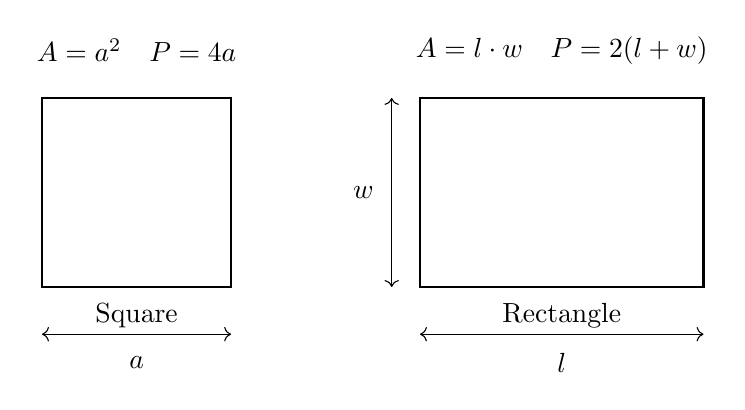
\begin{tikzpicture}[scale=1.2]
		% Square
		\draw[thick] (0,0) rectangle (2,2);
		\node at (1,-0.3) {Square};
		\draw[<->] (0,-0.5) -- (2,-0.5);
		\node at (1,-0.8) {\(a\)};
		\node at (1,2.5) {\(A = a^2 \quad P = 4a\)};

		% Rectangle
		\draw[thick] (4,0) rectangle (7,2);
		\node at (5.5,-0.3) {Rectangle};
		\draw[<->] (4,-0.5) -- (7,-0.5);
		\node at (5.5,-0.8) {\(l\)};
		\draw[<->] (3.7,0) -- (3.7,2);
		\node at (3.4,1) {\(w\)};
		\node at (5.5,2.5) {\(A = l \cdot w \quad P = 2(l+w)\)};
	\end{tikzpicture}
\end{center}

\subsection*{Circle and Triangle Types}
\begin{center}
	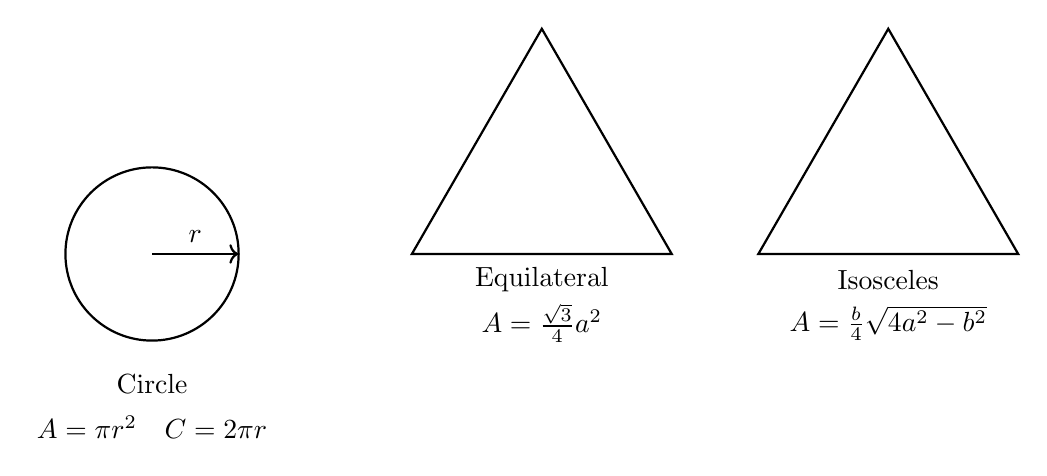
\begin{tikzpicture}[scale=1.1]
		% Circle
		\draw[thick] (0,0) circle(1cm);
		\draw[thick, ->] (0,0) -- (1,0);
		\node at (0.5,0.2) {\(r\)};
		\node at (0,-1.5) {Circle};
		\node at (0,-2) {\(A = \pi r^2 \quad C = 2\pi r\)};

		% Equilateral Triangle
		\draw[thick] (3,0) -- (4.5,2.6) -- (6,0) -- cycle;
		\node at (4.5,-0.3) {Equilateral};
		\node at (4.5,-0.8) {\(A = \frac{\sqrt{3}}{4} a^2\)};

		% Isosceles Triangle
		\draw[thick] (7,0) -- (8.5,2.6) -- (10,0) -- cycle;
		\node at (8.5,-0.3) {Isosceles};
		\node at (8.5,-0.8) {\(A = \frac{b}{4} \sqrt{4a^2 - b^2}\)};
	\end{tikzpicture}
\end{center}

\subsection*{Scalene Triangle, Trapezoid, Parallelogram}
\begin{center}
	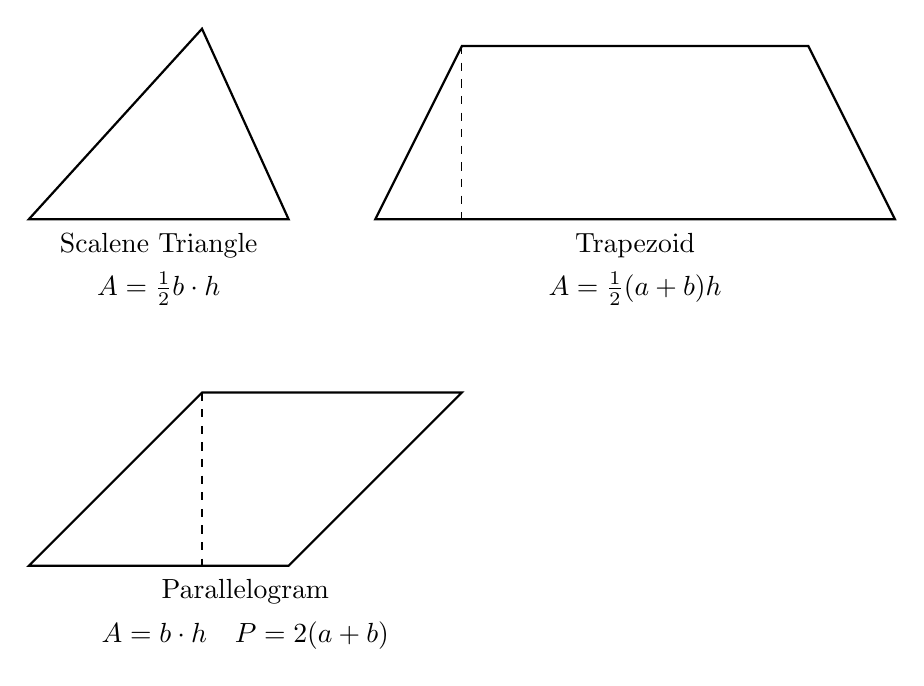
\begin{tikzpicture}[scale=1.1]
		% Scalene Triangle
		\draw[thick] (0,0) -- (2,2.2) -- (3,0) -- cycle;
		\node at (1.5,-0.3) {Scalene Triangle};
		\node at (1.5,-0.8) {\(A = \frac{1}{2} b \cdot h\)};

		% Trapezoid
		\draw[thick] (4,0) -- (5,2) -- (9,2) -- (10,0) -- cycle;
		\draw[dashed] (5,2) -- (5,0);
		\node at (7,-0.3) {Trapezoid};
		\node at (7,-0.8) {\(A = \frac{1}{2}(a+b)h\)};

		% Parallelogram
		\draw[thick] (0,-4) -- (2,-2) -- (5,-2) -- (3,-4) -- cycle;
		\draw[dashed] (2,-2) -- (2,-4);
		\node at (2.5,-4.3) {Parallelogram};
		\node at (2.5,-4.8) {\(A = b \cdot h \quad P = 2(a + b)\)};
	\end{tikzpicture}
\end{center}

\subsection{3D Geometric Figures with Formulas}

\subsubsection{Cube and Cylinder}
\begin{center}
	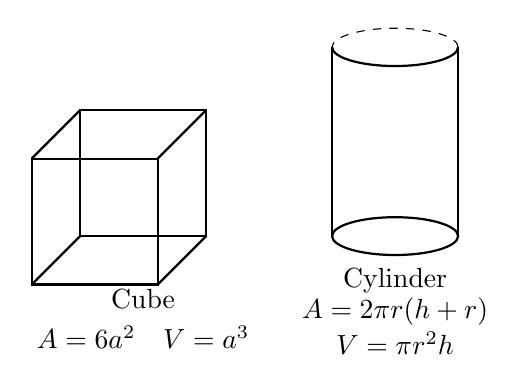
\begin{tikzpicture}[scale=0.8]
		% Cube
		\draw[thick] (0,0,0) -- (2,0,0) -- (2,2,0) -- (0,2,0) -- cycle;
		\draw[thick] (0,0,0) -- (0,0,2);
		\draw[thick] (2,0,0) -- (2,0,2);
		\draw[thick] (2,2,0) -- (2,2,2);
		\draw[thick] (0,2,0) -- (0,2,2);
		\draw[thick] (0,0,2) -- (2,0,2) -- (2,2,2) -- (0,2,2) -- cycle;
		\node at (1,-1) {Cube};
		\node at (1,-1.6) {\(A = 6a^2 \quad V = a^3\)};

		% Cylinder
		\begin{scope}[xshift=5cm]
			\draw[thick] (0,0) ellipse (1 and 0.3);
			\draw[thick] (-1,0) -- (-1,3);
			\draw[thick] (1,0) -- (1,3);
			\draw[thick] (-1,3) arc (180:360:1 and 0.3);
			\draw[dashed] (1,3) arc (0:180:1 and 0.3);
			\node at (0, -0.7) {Cylinder};
			\node at (0, -1.2) {\(A = 2\pi r(h + r)\)};
			\node at (0, -1.7) {\(V = \pi r^2 h\)};
		\end{scope}
	\end{tikzpicture}
\end{center}

\subsubsection{Cone and Sphere}
\begin{center}
	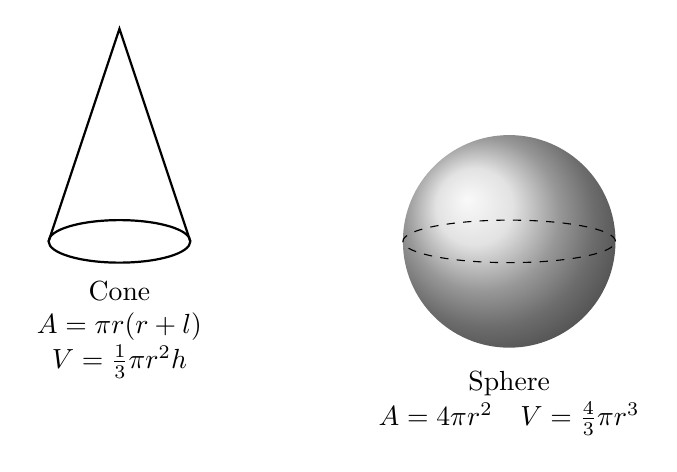
\begin{tikzpicture}[scale=0.9]
		% Cone
		\draw[thick] (0,0) ellipse (1 and 0.3);
		\draw[thick] (-1,0) -- (0,3) -- (1,0);
		\draw[dashed] (1,0) arc (0:180:1 and 0.3);
		\node at (0,-0.7) {Cone};
		\node at (0,-1.2) {\(A = \pi r(r + l)\)};
		\node at (0,-1.7) {\(V = \frac{1}{3} \pi r^2 h\)};

		% Sphere
		\begin{scope}[xshift=5.5cm]
			\shade[ball color=gray!30] (0,0) circle (1.5);
			\draw[dashed] (0,0) ellipse (1.5 and 0.3);
			\node at (0,-2) {Sphere};
			\node at (0,-2.5) {\(A = 4\pi r^2 \quad V = \frac{4}{3} \pi r^3\)};
		\end{scope}
	\end{tikzpicture}
\end{center}

\subsubsection{Pyramid and Prism}
\begin{center}
	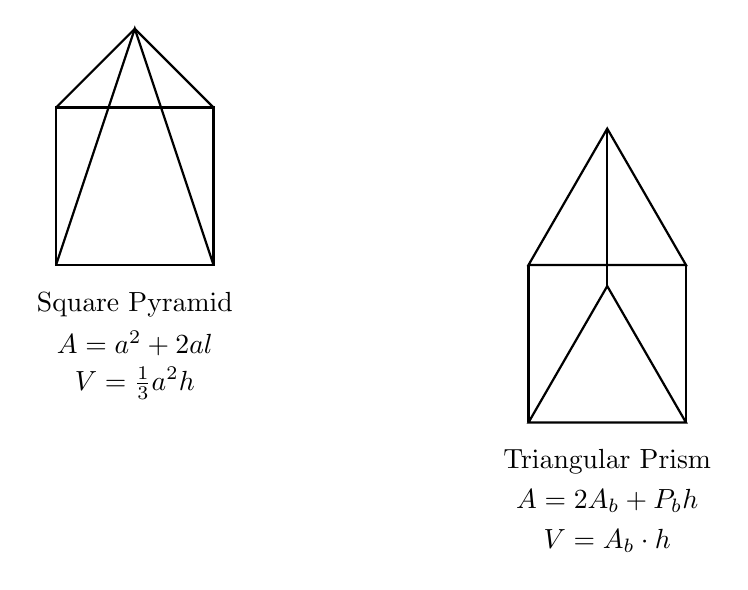
\begin{tikzpicture}[scale=1]
		% Square Pyramid
		\draw[thick] (0,0) -- (2,0) -- (2,2) -- (0,2) -- cycle;
		\draw[thick] (0,0) -- (1,3) -- (2,0);
		\draw[thick] (2,2) -- (1,3) -- (0,2);
		\node at (1,-0.5) {Square Pyramid};
		\node at (1,-1) {\(A = a^2 + 2al\)};
		\node at (1,-1.5) {\(V = \frac{1}{3}a^2 h\)};

		% Triangular Prism
		\begin{scope}[xshift=6cm]
			\draw[thick] (0,0) -- (2,0) -- (1,1.732) -- cycle;
			\draw[thick] (0,0) -- (0,-2);
			\draw[thick] (2,0) -- (2,-2);
			\draw[thick] (1,1.732) -- (1,-0.268);
			\draw[thick] (0,-2) -- (2,-2) -- (1,-0.268) -- cycle;
			\node at (1,-2.5) {Triangular Prism};
			\node at (1,-3) {\(A = 2A_b + P_b h\)};
			\node at (1,-3.5) {\(V = A_b \cdot h\)};
		\end{scope}
	\end{tikzpicture}
\end{center}

\subsection{Axioms of Euclidean Geometry}

Euclidean geometry is founded on a set of basic assumptions known as axioms or postulates, originally formulated by the Greek mathematician Euclid in his work \textit{Elements}. These axioms form the logical basis for plane geometry and include the following:

\begin{enumerate}
    \item \textbf{Axiom 1 (Line Postulate):} A straight line segment can be drawn joining any two points.
    
    \item \textbf{Axiom 2 (Extension Postulate):} Any straight line segment can be extended indefinitely in a straight line.
    
    \item \textbf{Axiom 3 (Circle Postulate):} Given any straight line segment, a circle can be drawn having the segment as radius and one endpoint as center.
    
    \item \textbf{Axiom 4 (Right Angle Postulate):} All right angles are congruent.
    
    \item \textbf{Axiom 5 (Parallel Postulate):} If a line segment intersects two straight lines and makes the interior angles on the same side less than two right angles, then the two lines, if extended indefinitely, meet on that side.
\end{enumerate}

These five postulates define the framework of classical geometry in a flat (Euclidean) space. Notably, the fifth postulate—the parallel postulate—has been the subject of much scrutiny and led to the development of non-Euclidean geometries when it was altered or replaced.

\subsection{Types of Angles and Angle Relationships}





\section{Constructing Triangles from Angles and Sides}
A triangle can be uniquely determined (up to congruence) using different combinations of sides and angles. The main construction cases are as follows:

\subsection{SSS (Side-Side-Side)}
A triangle is uniquely determined if all three sides are known.
\begin{center}
\begin{tikzpicture}[scale=1]
\draw[thick] (0,0) -- (5,0) node[midway, below] {$c$};
\draw[thick] (0,0) -- (2,3.5) node[midway, left] {$b$};
\draw[thick] (5,0) -- (2,3.5) node[midway, right] {$a$};
\node[below left] at (0,0) {$A$};
\node[below right] at (5,0) {$B$};
\node[above] at (2,3.5) {$C$};
\end{tikzpicture}
\end{center}

\subsection{SAS (Side-Angle-Side)}
A triangle is uniquely determined if two sides and the included angle are known.
\begin{center}
\begin{tikzpicture}[scale=1]
\coordinate (A) at (0,0);
\coordinate (B) at (5,0);
\coordinate (C) at (1.8,3);
\draw[thick] (A) -- (B) node[midway, below] {$c$};
\draw[thick] (A) -- (C) node[midway, left] {$b$};
\draw[thick] (B) -- (C) node[midway, right] {$a$};
\pic["$\theta$", draw=black, angle radius=1cm, angle eccentricity=1.3] {angle=B--A--C};
\node[below left] at (A) {$A$};
\node[below right] at (B) {$B$};
\node[above] at (C) {$C$};
\end{tikzpicture}
\end{center}

\subsection{ASA (Angle-Side-Angle)}
A triangle is uniquely determined if two angles and the included side are known.
\begin{center}
\begin{tikzpicture}[scale=1]
\coordinate (A) at (0,0);
\coordinate (B) at (5,0);
\coordinate (C) at (2,3.5);
\draw[thick] (A) -- (B) node[midway, below] {$c$};
\draw[thick] (A) -- (C);
\draw[thick] (B) -- (C);
\pic["$\alpha$", draw=black, angle radius=1cm, angle eccentricity=1.4] {angle=B--A--C};
\pic["$\beta$", draw=black, angle radius=1cm, angle eccentricity=1.4] {angle=C--B--A};
\node[below left] at (A) {$A$};
\node[below right] at (B) {$B$};
\node[above] at (C) {$C$};
\end{tikzpicture}
\end{center}

\subsection{AAS (Angle-Angle-Side)}
A triangle is uniquely determined if two angles and a non-included side are known.
\begin{center}
\begin{tikzpicture}[scale=1]
\coordinate (A) at (0,0);
\coordinate (C) at (4,0);
\coordinate (B) at (2,3);
\draw[thick] (A) -- (C) node[midway, below] {$b$};
\draw[thick] (A) -- (B);
\draw[thick] (B) -- (C);
\pic["$\alpha$", draw=black, angle radius=1cm, angle eccentricity=1.4] {angle=C--A--B};
\pic["$\beta$", draw=black, angle radius=1cm, angle eccentricity=1.4] {angle=A--C--B};
\node[below left] at (A) {$A$};
\node[below right] at (C) {$C$};
\node[above] at (B) {$B$};
\end{tikzpicture}
\end{center}

\subsection{SSA (Side-Side-Angle)}
Two sides and a non-included angle do \textbf{not always} determine a unique triangle. This case is ambiguous and can result in:
\begin{itemize}
    \item One triangle (when the opposite side is long enough),
    \item Two triangles (ambiguous case),
    \item No triangle (when the side is too short).
\end{itemize}
\begin{center}
\begin{tikzpicture}[scale=1]
\coordinate (A) at (0,0);
\coordinate (C) at (4,0);
\coordinate (B1) at (2,3); % triangle 1
\coordinate (B2) at (2,-2); % triangle 2
\draw[thick] (A) -- (C) node[midway, below] {$c$};
\draw[thick] (A) -- (B1) node[midway, left] {$b$};
\draw[thick] (A) -- (B2) node[midway, left] {$b$};
\draw[thick, dashed] (B2) -- (C);
\draw[thick] (B1) -- (C);
\pic["$\alpha$", draw=black, angle radius=1cm, angle eccentricity=1.4] {angle=C--A--B1};
\node[below left] at (A) {$A$};
\node[below right] at (C) {$C$};
\node[above] at (B1) {$B_1$};
\node[below] at (B2) {$B_2$};
\end{tikzpicture}
\end{center}

\subsection{Intercept Theorems}

The intercept theorems describe relationships between segment lengths when two rays from a point intersect two parallel lines. They are based on similar triangles and allow us to calculate unknown lengths using proportions.

\subsubsection{First Intercept Theorem}

If two rays start from a common point and are intersected by two parallel lines, then:

\[
	\frac{a}{a'} = \frac{b}{b'}
\]

\noindent where \(a\) and \(b\) are segments on one ray, and \(a'\), \(b'\) are the corresponding segments on the other ray.

\begin{center}
	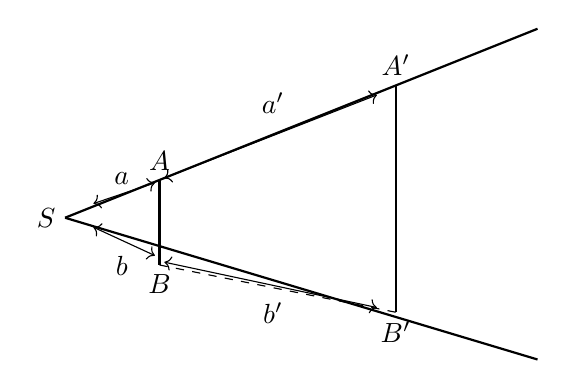
\begin{tikzpicture}[scale=1.2]
		% Rays
		\draw[thick] (0,0) -- (5,2); % upper ray
		\draw[thick] (0,0) -- (5,-1.5); % lower ray

		% Parallels
		\draw[thick] (1,0.4) -- (1,-0.5);
		\draw[thick] (3.5,1.4) -- (3.5,-1);

		% Points
		\node at (-0.2,0) {\(S\)};
		\node[above] at (1,0.4) {\(A\)};
		\node[below] at (1,-0.5) {\(B\)};
		\node[above] at (3.5,1.4) {\(A'\)};
		\node[below] at (3.5,-1) {\(B'\)};

		% Helper lines
		\draw[dashed] (1,0.4) -- (3.5,1.4);
		\draw[dashed] (1,-0.5) -- (3.5,-1);

		% Length labels
		\draw[<->] (0.3,0.15) -- (0.95,0.37);
		\node[above] at (0.6,0.25) {\(a\)};
		\draw[<->] (1.05,0.42) -- (3.3,1.3);
		\node[above] at (2.2,1) {\(a'\)};

		\draw[<->] (0.3,-0.1) -- (0.95,-0.4);
		\node[below] at (0.6,-0.3) {\(b\)};
		\draw[<->] (1.05,-0.47) -- (3.3,-0.95);
		\node[below] at (2.2,-0.8) {\(b'\)};
	\end{tikzpicture}
\end{center}

\subsubsection{Second Intercept Theorem (General Form)}

If a ray intersects two parallel lines, the segments from the origin point to the lines are in the same ratio as the segments along the parallels:

\[
	\frac{SA}{SA'} = \frac{SB}{SB'} \quad \text{and} \quad \frac{AB}{A'B'} = \frac{SA}{SA'}
\]

\begin{center}
	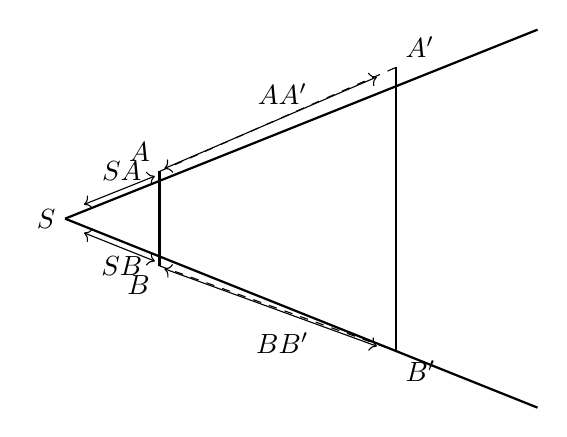
\begin{tikzpicture}[scale=1.2]
		% Rays
		\draw[thick] (0,0) -- (5,2); % upper ray
		\draw[thick] (0,0) -- (5,-2); % lower ray

		% Parallels
		\draw[thick] (1,0.5) -- (1,-0.5);
		\draw[thick] (3.5,1.6) -- (3.5,-1.4);

		% Points
		\node at (-0.2,0) {\(S\)};
		\node[above left] at (1,0.5) {\(A\)};
		\node[below left] at (1,-0.5) {\(B\)};
		\node[above right] at (3.5,1.6) {\(A'\)};
		\node[below right] at (3.5,-1.4) {\(B'\)};

		% Helper lines
		\draw[dashed] (1,0.5) -- (3.5,1.6);
		\draw[dashed] (1,-0.5) -- (3.5,-1.4);
		\draw[dashed] (1,0.5) -- (1,-0.5);
		\draw[dashed] (3.5,1.6) -- (3.5,-1.4);

		% Length labels
		\draw[<->] (0.2,0.15) -- (0.95,0.45);
		\node[above] at (0.6,0.3) {\(SA\)};
		\draw[<->] (1.05,0.53) -- (3.3,1.5);
		\node[above] at (2.3,1.1) {\(AA'\)};

		\draw[<->] (0.2,-0.15) -- (0.95,-0.45);
		\node[below] at (0.6,-0.3) {\(SB\)};
		\draw[<->] (1.05,-0.53) -- (3.3,-1.35);
		\node[below] at (2.3,-1.1) {\(BB'\)};
	\end{tikzpicture}
\end{center}

\newpage


\input{src/Geometry_and_Trig/Trigonometry.tex}


\section{Linear Systems of Equations}

In this section, we will discuss the solution of linear systems of equations. A linear system of equations is a set of equations that can be expressed in the form:
\begin{align*}
a_{11}x_1 + a_{12}x_2 + \cdots + a_{1n}x_n & = b_1  \\
a_{21}x_1 + a_{22}x_2 + \cdots + a_{2n}x_n & = b_2  \\
& \vdots \\
a_{m1}x_1 + a_{m2}x_2 + \cdots + a_{mn}x_n & = b_m
\end{align*}

where \( a_{ij} \) are the coefficients of the variables \( x_j \), and \( b_i \) are the constants on the right-hand side of the equations. The goal is to find the values of \( x_1, x_2, \ldots, x_n \) that satisfy all equations simultaneously.

\subsection{Matrix Representation}

A linear system can be represented in matrix form as:
\begin{equation*}
	A \mathbf{x} = \mathbf{b}
\end{equation*}
where \( A \) is the coefficient matrix, \( \mathbf{x} \) is the vector of variables, and \( \mathbf{b} \) is the vector of constants. The coefficient matrix \( A \) is an \( m \times n \) matrix, where \( m \) is the number of equations and \( n \) is the number of variables.
The vector \( \mathbf{x} \) is an \( n \times 1 \) column vector, and the vector \( \mathbf{b} \) is an \( m \times 1 \) column vector. The system can be solved using various methods, including:

\begin{itemize}[label=\(-\)]
	\item Gaussian elimination
	\item LU decomposition
	\item Matrix inversion (if \( A \) is square and invertible)
	\item Iterative methods (e.g., Jacobi, Gauss-Seidel)
	\item Special methods for sparse matrices
	\item Special methods for structured matrices (e.g., banded, Toeplitz)
	\item Special methods for large-scale problems (e.g., conjugate gradient, GMRES)
\end{itemize}

\subsection{Gaussian Elimination}

Gaussian elimination is a method for solving linear systems by transforming the system into an upper triangular form. The steps involved in Gaussian elimination are:
\begin{enumerate}
	\item Forward elimination: Transform the system into an upper triangular form by eliminating the variables from the equations.
	\item Back substitution: Solve for the variables starting from the last equation and substituting back into the previous equations.
\end{enumerate}
The forward elimination process involves performing row operations on the augmented matrix \([A | \mathbf{b}]\) to create zeros below the diagonal. The row operations include:
\begin{itemize}[label=\(-\)]
	\item Swapping two rows
	\item Multiplying a row by a non-zero scalar
	\item Adding or subtracting a multiple of one row from another row
\end{itemize}
Once the matrix is in upper triangular form, back substitution is used to find the values of the variables. The last equation gives the value of the last variable, which can then be substituted into the previous equations to find the other variables.

\subsection{Gauss-Jordan Elimination}

Gauss-Jordan elimination is an extension of Gaussian elimination that transforms the matrix into reduced row echelon form (RREF). In RREF, each leading entry in a row is 1, and all entries above and below the leading entry are zeros. The steps involved in Gauss-Jordan elimination are:
\begin{enumerate}
	\item Forward elimination: Transform the system into an upper triangular form.
	\item Back substitution: Transform the upper triangular matrix into RREF by eliminating the entries above the leading 1s.
	\item Solve for the variables directly from the RREF matrix.
\end{enumerate}
The Gauss-Jordan elimination method is particularly useful for finding the inverse of a matrix, as it can be applied to the augmented matrix \([A | I]\), where \(I\) is the identity matrix. If the left side of the augmented matrix becomes \(I\), then the right side will be the inverse of \(A\).

\textbf{Example:} Solve the following system of equations using Gaussian elimination:
\begin{align*}
	2x + 3y + z  & = 1 \\
	4x + y - z   & = 2 \\
	-2x + y + 3z & = 3
\end{align*}
\textbf{Solution:} The augmented matrix for the system is:
\begin{equation*}
	\begin{bmatrix}
		2  & 3 & 1  & | & 1 \\
		4  & 1 & -1 & | & 2 \\
		-2 & 1 & 3  & | & 3
	\end{bmatrix}
\end{equation*}
Performing row operations to eliminate the variables, we can transform the matrix into upper triangular form:
\begin{equation*}
	\begin{bmatrix}
		1 & \frac{3}{2} & \frac{1}{2} & | & \frac{1}{2} \\
		0 & -5          & -3          & | & 0           \\
		0 & 0           & 1           & | & 1
	\end{bmatrix}
\end{equation*}
Now, we can perform back substitution to find the values of \(x\), \(y\), and \(z\):
\begin{align*}
	z           & = 1                           \\
	-5y - 3z    & = 0 \implies y = -\frac{3}{5} \\
	2x + 3y + z & = 1 \implies x = \frac{1}{5}
\end{align*}
Thus, the solution to the system is:
\begin{align*}
	x & = \frac{1}{5}  \\
	y & = -\frac{3}{5} \\
	z & = 1
\end{align*}

\subsection{Homogeneous Linear Equations}

A linear equation is said to be \emph{homogeneous} if its constant term is zero. That is, it can be written in the form:
\[
	a_1x_1 + a_2x_2 + \cdots + a_nx_n = 0
\]

Such equations always have at least the trivial solution \(x_1 = x_2 = \cdots = x_n = 0\).

\subsection{Particular Solution}
A particular solution to a linear system of equations is a specific solution that satisfies the system. It can be found using various methods, including substitution, elimination, or matrix methods. A particular solution is not unique; there may be multiple particular solutions depending on the system.
A particular solution can be found by substituting specific values for the variables and solving for the remaining variables. For example, in the system
\begin{align*}
	2x + 3y & = 5 \\
	4x - y  & = 1
\end{align*}
we can substitute \(x = 1\) into the first equation to find \(y\):
\begin{align*}
	2(1) + 3y & = 5 \\
	3y        & = 3 \\
	y         & = 1
\end{align*}
Thus, \((x, y) = (1, 1)\) is a particular solution to the system. However, this is not the only solution; other values of \(x\) may yield different values of \(y\).

\subsection{General = Particular + Homogeneous}
The general solution of a linear system of equations is the complete set of solutions that satisfy the system. It can be expressed as the sum of a particular solution and the general solution of the associated homogeneous system.
The general solution can be written as:
\begin{equation*}
	\mathbf{x} = \mathbf{x}_p + \mathbf{x}_h
\end{equation*}
where \( \mathbf{x}_p \) is a particular solution to the non-homogeneous system, and \( \mathbf{x}_h \) is the general solution to the homogeneous system.
The homogeneous system is obtained by setting the right-hand side of the equations to zero:
\begin{equation*}
	A \mathbf{x} = \mathbf{0}
\end{equation*}

 The theoreme says:

Any linear system's solution set has the form:
\[
	\left\{ \vec{p} + c_1\vec{\beta}_1 + \cdots + c_k\vec{\beta}_k \;\middle|\; c_1, \ldots, c_k \in \mathbb{R} \right\}
\]

where \(\vec{p}\) is a particular solution to the system, and the vectors \(\vec{\beta}_1, \ldots, \vec{\beta}_k\) form a basis of the solution space to the corresponding homogeneous system. The number \(k\) equals the number of \textbf{free variables} the system has after applying Gaussian elimination.

\subsection{Linear Combination Lemma}
Any linear combination of linear combinations is a linear combination.

\subsection{Example: Gaussian Elimination with 3 Equations and 4 Unknowns}

Consider the following system of linear equations:

\begin{align*}
	x_1 + 2x_2 + x_3 + x_4   & = 4  \\
	2x_1 + 5x_2 + x_3 + 3x_4 & = 10 \\
	x_1 + 3x_2 + 2x_3 + 2x_4 & = 7
\end{align*}

\subsubsection*{Step 1: Augmented Matrix}

\[
	\begin{bmatrix}
		1 & 2 & 1 & 1 & 4  \\
		2 & 5 & 1 & 3 & 10 \\
		1 & 3 & 2 & 2 & 7  \\
	\end{bmatrix}
\]

\subsubsection*{Step 2: Eliminate below pivot in column 1}

\begin{itemize}[label=\(-\)]
	\item Row 2 = Row 2 - 2 × Row 1
	\item Row 3 = Row 3 - Row 1
\end{itemize}

\[
	\begin{bmatrix}
		1 & 2 & 1  & 1 & 4 \\
		0 & 1 & -1 & 1 & 2 \\
		0 & 1 & 1  & 1 & 3 \\
	\end{bmatrix}
\]

\subsubsection*{Step 3: Eliminate below pivot in column 2}

\begin{itemize}[label=\(-\)]
	\item Row 3 = Row 3 - Row 2
\end{itemize}

\[
	\begin{bmatrix}
		1 & 2 & 1  & 1 & 4 \\
		0 & 1 & -1 & 1 & 2 \\
		0 & 0 & 2  & 0 & 1 \\
	\end{bmatrix}
\]

\subsubsection*{Step 4: Back Substitution}

From Row 3:
\[
	2x_3 = 1 \Rightarrow x_3 = \frac{1}{2}
\]

From Row 2:
\[
	x_2 - x_3 + x_4 = 2 \Rightarrow x_2 = 2 + x_3 - x_4 = 2 + \frac{1}{2} - x_4 = \frac{5}{2} - x_4
\]

From Row 1:
\[
	x_1 + 2x_2 + x_3 + x_4 = 4
	\Rightarrow x_1 = 4 - 2x_2 - x_3 - x_4
\]
Substitute:
\[
	x_1 = 4 - 2\left( \frac{5}{2} - x_4 \right) - \frac{1}{2} - x_4
	= 4 - 5 + 2x_4 - \frac{1}{2} - x_4
	= -1 - \frac{1}{2} + x_4 = -\frac{3}{2} + x_4
\]

\subsubsection*{General Solution}

Let \(x_4 = t\) (free variable), then:

\[
	\begin{aligned}
		x_1 & = -\frac{3}{2} + t \\
		x_2 & = \frac{5}{2} - t  \\
		x_3 & = \frac{1}{2}      \\
		x_4 & = t
	\end{aligned}
	\quad \text{with } t \in \mathbb{R}
\]

\textbf{Solution Set:}

\[
	\left\{
	\begin{pmatrix}
		-\frac{3}{2} \\ \frac{5}{2} \\ \frac{1}{2} \\ 0
	\end{pmatrix}
	+ t \cdot
	\begin{pmatrix}
		1 \\ -1 \\ 0 \\ 1
	\end{pmatrix}
	\;\middle|\; t \in \mathbb{R}
	\right\}
\]

\subsection{The Determinant, the cross product and the solutions of linear Systems of Equations}
A linear system of three equation has the following properties:

\begin{itemize}[label=\(-\)]
	\item There is a unique solution if the determinant of the coefficient matrix is non-zero. 
	\[\langle (a x b), c\rangle = \det(a,b,c) \ne 0\]
	\item There are infinitely many solutions if the determinant of the coefficient matrix is zero.
	\[\langle (a x b), c\rangle = \det(a,b,c) = 0\]
	\item There is no solution if the determinant of the coefficient matrix is zero and the system is inconsistent.
	\[\langle (a x b), c\rangle = 0\]
\end{itemize}

\newpage
\input{src/Linear_Algebra/Analytical_Geometry.tex}
\section{Algebraic Structures}

\subsection{Introduction}

Algebraic structures are mathematical systems consisting of a set equipped with one or more operations that satisfy certain axioms. They provide a unified language to study various objects in mathematics, from numbers and matrices to functions and vector spaces. Understanding these structures is fundamental in abstract algebra and has applications in computer science, cryptography, coding theory, and physics.

\subsection{Operations: Internal and External}

An \textbf{internal composition law} is a binary operation that takes two elements from a set and returns another element in the same set. Formally, for a set \(S\) and operation \(\circ\), we have:
\[
\circ: S \times S \rightarrow S
\]

An \textbf{external composition law} involves a second set acting on the structure, such as scalar multiplication in vector spaces:
\[
\cdot: K \times V \rightarrow V
\]
where \(K\) is a field and \(V\) is a vector space.

\subsection{Properties of Operations}

Let \(\ast\) be a binary operation on a set \(S\). The most important properties include:

\begin{itemize}[label=\(-\)]
    \item \textbf{Associativity:} \((a \ast b) \ast c = a \ast (b \ast c)\) for all \(a,b,c \in S\)
    \item \textbf{Commutativity:} \(a \ast b = b \ast a\) for all \(a,b \in S\)
    \item \textbf{Identity Element:} There exists \(e \in S\) such that \(a \ast e = e \ast a = a\) for all \(a \in S\)
    \item \textbf{Inverse Element:} For every \(a \in S\), there exists \(a^{-1} \in S\) such that \(a \ast a^{-1} = a^{-1} \ast a = e\)
    \item \textbf{Distributivity:} \(a \circ (b \bullet c) = (a \circ b) \bullet (a \circ c)\) and/or \((b \bullet c) \circ a = (b \circ a) \bullet (c \circ a)\)
\end{itemize}

\subsection{Homomorphisms and Isomorphisms}

Let \((G, \oplus)\) and \((H, \oplus')\) be two algebraic structures.

\begin{itemize}[label=\(-\)]
    \item A \textbf{homomorphism} is a function \(\varphi: G \rightarrow H\) such that:
    \[
    \varphi(a \oplus b) = \varphi(a) \oplus' \varphi(b), \quad \forall a,b \in G
    \]
    
    \item An \textbf{isomorphism} is a bijective homomorphism. If such a map exists, we say the structures are \textbf{isomorphic}, written as \(G \cong H\).
\end{itemize}

\subsection{Common Algebraic Structures}

The following table lists common algebraic structures along with their notation and defining properties. Let \(\oplus\) denote the additive operation and \(\odot\) the multiplicative one:

\begin{center}
\renewcommand{\arraystretch}{1.4}
\begin{tabular}{|c|c|l|}
\hline
\textbf{Name} & \textbf{Notation} & \textbf{Properties} \\
\hline
\textbf{Semigroup} & \((S, \oplus)\) & Associative \\
\hline
\textbf{Monoid} & \((M, \oplus)\) & Associative, Identity element \\
\hline
\textbf{Group} & \((G, \oplus)\) & Associative, Identity, Inverses \\
\hline
\textbf{Abelian Group} & \((A, \oplus)\) & Group + Commutativity \\
\hline
\textbf{Ring} & \((R, \oplus, \odot)\) & \begin{tabular}[c]{@{}l@{}}\((R, \oplus)\) is an abelian group,\\ \((R, \odot)\) is a semigroup,\\ Distributivity: \(a \odot (b \oplus c) = a \odot b \oplus a \odot c\)\end{tabular} \\
\hline
\textbf{Commutative Ring} & \((R, \oplus, \odot)\) & Ring + \((R, \odot)\) is commutative \\
\hline
\textbf{Field} & \((K, \oplus, \odot)\) & \begin{tabular}[c]{@{}l@{}}Commutative Ring +\\ \((K \setminus \{0\}, \odot)\) is an abelian group\end{tabular} \\
\hline
\textbf{Vector Space} & \((V, \oplus, \cdot)\) & \begin{tabular}[c]{@{}l@{}}\((V, \oplus)\) is an abelian group,\\ \(\cdot: K \times V \to V\) (scalar mult.),\\ Distributivity, associativity, identities\end{tabular} \\
\hline
\end{tabular}
\end{center}

\newpage

\section{Vector Spaces}

A \textbf{vector space} is a set \(V\) with two operations, vector addition and scalar multiplication, such that:

\begin{enumerate}[label=\Roman*.]
	\item The set \(V\) is closed under vector addition.
	\item The set \(V\) is closed under scalar multiplication.
	\item Vector addition is commutative.
	\item Vector addition is associative.
	\item There exists a zero vector \(\vec{0} \in V\) such that \(\vec{v} + \vec{0} = \vec{v}\) for all \(\vec{v} \in V\).
	\item For every vector \(\vec{v} \in V\), there exists a vector \(-\vec{v} \in V\) such that \(\vec{v} + (-\vec{v}) = \vec{0}\).
	\item Scalar multiplication is distributive with respect to vector addition: \(a(\vec{u} + \vec{v}) = a\vec{u} + a\vec{v}\) for all \(a \in F\) and \(\vec{u}, \vec{v} \in V\).
	\item Scalar multiplication is distributive with respect to field addition: \((a + b)\vec{v} = a\vec{v} + b\vec{v}\) for all \(a, b \in F\) and \(\vec{v} \in V\).
	\item Scalar multiplication is associative: \(a(b\vec{v}) = (ab)\vec{v}\) for all \(a, b \in F\) and \(\vec{v} \in V\).
	\item The multiplicative identity acts as a scalar: \(1\vec{v} = \vec{v}\) for all \(\vec{v} \in V\).
\end{enumerate}
The set \(F\) is a field, and the elements of \(V\) are called \textbf{vectors}.

\textbf{Examples:}

\begin{enumerate}
	\item The set of all \(n\)-tuples of real numbers \(\mathbb{R}^n\) is a vector space over the field of real numbers \(\mathbb{R}\).
	\item The set of all polynomials of degree less than or equal to \(n\) is a vector space over the field of real numbers \(\mathbb{R}\).
	\item The set of all continuous functions from \(\mathbb{R}\) to \(\mathbb{R}\) is a vector space over the field of real numbers \(\mathbb{R}\).
	\item The set of all \(m \times n\) matrices with real entries is a vector space over the field of real numbers \(\mathbb{R}\).
\end{enumerate}

\subsection{Subspaces}

A subset \(W\) of a vector space \(V\) is a \textbf{subspace} of \(V\) if:

\begin{enumerate}[label=\Roman*.]
	\item The zero vector \(\vec{0} \in W\).
	\item For all \(\vec{u}, \vec{v} \in W\), \(\vec{u} + \vec{v} \in W\).
	\item For all \(a \in F\) and \(\vec{v} \in W\), \(a\vec{v} \in W\).
\end{enumerate}
If \(W\) is a subspace of \(V\), we write \(W \subseteq V\).

\textbf{Note:} The intersection of two subspaces is also a subspace.

\subsection{Linear Combinations}

A \textbf{linear combination} of vectors \(\vec{v}_1, \vec{v}_2, \ldots, \vec{v}_n\) in a vector space \(V\) is an expression of
the form:
\[
	a_1\vec{v}_1 + a_2\vec{v}_2 + \ldots + a_n\vec{v}_n
\]
where \(a_1, a_2, \ldots, a_n\) are scalars from the field \(F\).
The set of all linear combinations of a set of vectors \(\{\vec{v}_1, \vec{v}_2, \ldots, \vec{v}_n\}\) is called the \textbf{span} of those vectors,
denoted by \(\text{span}(\vec{v}_1, \vec{v}_2, \ldots, \vec{v}_n)\).
The span of a set of vectors is a subspace of the vector space \(V\).
\textbf{Note:} The span of a set of vectors is the smallest subspace containing those vectors.

\subsection{Properties of the subspaces}

\begin{itemize}[label=\(-\)]
	\item The intersection of two subspaces is a subspace.
	\item The union of two subspaces is not necessarily a subspace.
	\item The sum of two subspaces \(U\) and \(W\) is defined as:
	      \[
		      U + W = \{\vec{u} + \vec{w} : \vec{u} \in U, \vec{w} \in W\}
	      \]
	      The sum of two subspaces is a subspace.
\end{itemize}
\textbf{Note:} The sum of two subspaces is the smallest subspace containing both subspaces.
\begin{itemize}[label=\(-\)]
	\item The direct sum of two subspaces \(U\) and \(W\) is defined as:
	      \[
		      U \oplus W = \{\vec{u} + \vec{w} : \vec{u} \in U, \vec{w} \in W\}
	      \]
	      The direct sum of two subspaces is a subspace.
	\item The direct sum of two subspaces is the smallest subspace containing both subspaces, such that \(U \cap W = \{\vec{0}\}\).
	\item The direct sum of two subspaces is denoted by \(U \oplus W\).
\end{itemize}

\subsection{Linear Independence}

A set of vectors \(\{\vec{v}_1, \vec{v}_2, \ldots, \vec{v}_n\}\) in a vector space \(V\) is said to be \textbf{linearly independent} if the only solution to the equation:
\[
	\lambda_1\vec{v}_1 + \lambda_2\vec{v}_2 + \ldots + \lambda_n\vec{v}_n = 0
\]
or
\[
	\sum_{i=1}^n \lambda_i \vec{v}_i = 0
\]
is \(a_1 = a_2 = \ldots = a_n = 0\).
If there exists a non-trivial solution to this equation, then the set of vectors is said to be \textbf{linearly dependent}.
A set of vectors is linearly independent if and only if the only linear combination of those vectors that equals the zero vector is the trivial combination where all coefficients are zero.

\subsubsection{Properties of the linear independence}

\begin{itemize}[label=\(-\)]
	\item A set of vectors \(\{\vec{v}_1, \vec{v}_2, \ldots, \vec{v}_n\}\) is linearly independent if and only if the only linear combination of those vectors that equals the zero vector is the trivial combination where all coefficients are zero.
	\item If a set of vectors \(\{\vec{v}_1, \vec{v}_2, \ldots, \vec{v}_n\}\) is linearly independent, then any subset of that set is also linearly independent.
	\item If a set of vectors \(\{\vec{v}_1, \vec{v}_2, \ldots, \vec{v}_n\}\) is linearly dependent, then at least one vector in that set can be expressed as a linear combination of the others.
\end{itemize}

\subsection{Base}

\begin{itemize}[label=\(-\)]
\item A \textbf{base} of a vector space \(V\) is a set of vectors \(\{\vec{v}_1, \vec{v}_2, \ldots, \vec{v}_n\}\) that is linearly independent and spans the vector space \(V\).
\item The number of vectors in a base of a vector space is called the \textbf{dimension} of the vector space.
\item The dimension of a vector space \(V\) is denoted by \(\dim(V)\).
\item If \(V\) has a finite base, then it is said to be \textbf{finite-dimensional}.
\item If \(V\) does not have a finite base, then it is said to be \textbf{infinite-dimensional}.
\end{itemize}

\subsection{Dimension}
The \textbf{dimension} of a vector space \(V\) is the number of vectors in a base of \(V\).

\begin{itemize}[label=\(-\)]
	\item The dimension of a vector space is denoted by \(\dim(V)\).
	\item The dimension of a vector space can be finite or infinite.
	\item If the dimension of a vector space is finite, then it is said to be \textbf{finite-dimensional}.
	\item If the dimension of a vector space is infinite, then it is said to be \textbf{infinite-dimensional}.
\end{itemize}

\subsubsection{How to find the base of a set vector}
To find the base of a set of vectors, we can use the following steps:
\begin{enumerate}
	\item Write the vectors as columns of a matrix.
	\item Row reduce the matrix to echelon form.
	\item The non-zero rows of the echelon form matrix correspond to the base of the vector space spanned by the original set of vectors.
\end{enumerate}
The number of non-zero rows in the echelon form matrix is equal to the dimension of the vector space spanned by the original set of vectors.

\textbf{Note:} The base of a vector space is not unique. Different bases can span the same vector space.

\subsection{Basis Extension Theorem}

Let \(V\) be a vector space over a field \(K\), and let 
\[
v_1, \ldots, v_r,\quad w_1, \ldots, w_s \in V.
\]
Suppose that \((v_1, \ldots, v_r)\) is a linearly independent tuple and that
\[
\text{span}(v_1, \ldots, v_r, w_1, \ldots, w_s) = V.
\]
Then it is possible to extend \((v_1, \ldots, v_r)\) to a basis of \(V\) by possibly adding suitable vectors from the set \(\{w_1, \ldots, w_s\}\).

\subsubsection*{Proof}

If \(\text{span}(v_1, \ldots, v_r) = V\), the statement is obvious. So assume
\[
\text{span}(v_1, \ldots, v_r) \neq V.
\]

Then there exists at least one \(w_i\) such that \(w_i \notin \text{span}(v_1, \ldots, v_r)\); otherwise, if all \(w_i \in \text{span}(v_1, \ldots, v_r)\), then
\[
\text{span}(v_1, \ldots, v_r, w_1, \ldots, w_s) = \text{span}(v_1, \ldots, v_r) = V,
\]
which contradicts our assumption that \(\text{span}(v_1, \ldots, v_r) \neq V\).

The tuple \((w_i, v_1, \ldots, v_r)\) is linearly independent, because from
\[
\sum_{j=1}^r \lambda_j v_j + \lambda w_i = 0
\]
it follows that \(\lambda = 0\) (since \(w_i \notin \text{span}(v_1, \ldots, v_r)\)), and then also \(\lambda_j = 0\) for all \(j\) because the \(v_j\) are linearly independent.

Possibly, \((w_i, v_1, \ldots, v_r)\) is still not a basis of \(V\). Then we repeat the previous step and keep adding further \(w_i\) until the tuple extends \((v_1, \ldots, v_r)\) to a basis of \(V\). This process terminates after finitely many steps, since
\[
\text{span}(v_1, \ldots, v_r, w_1, \ldots, w_s) = V.
\]
\QED

\textbf{Note:} Every finitely generated vector space \(V\) has a basis.

\subsection{Exchange Lemma}

Let \((v_1, \ldots, v_n)\) and \((w_1, \ldots, w_m)\) be bases of a vector space \(V\). Then, for every \(v_i\), there exists a \(w_j\) such that if we replace \(v_i\) by \(w_j\) in the tuple \((v_1, \ldots, v_n)\), it still forms a basis of \(V\).

\textbf{Proof:}

Let \((v_1, \ldots, v_n)\) and \((w_1, \ldots, w_m)\) be two bases of \(V\). Suppose we remove \(v_i\) from the first basis. The truncated tuple \((v_1, \ldots, v_{i-1}, v_{i+1}, \ldots, v_n)\) satisfies
\[
\text{span}(v_1, \ldots, v_{i-1}, v_{i+1}, \ldots, v_n) \neq V,
\]
because if \(\text{span}(v_1, \ldots, v_{i-1}, v_{i+1}, \ldots, v_n) = V\), then \(v_i\) would lie in the span of the remaining vectors and could be written as a linear combination of them. This would contradict the assumption that \((v_1, \ldots, v_n)\) is linearly independent and a basis of \(V\).

By the Basis Extension Theorem, we can extend the truncated tuple \((v_1, \ldots, v_{i-1}, v_{i+1}, \ldots, v_n)\) to a basis of \(V\) by adding vectors from \((v_1, \ldots, v_{i-1}, v_{i+1}, \ldots, v_n, w_1, \ldots, w_m)\). Therefore, by the Basis Extension Theorem, there exists a \(w_j\) such that
\[
w_j \notin \text{span}(v_1, \ldots, v_{i-1}, v_{i+1}, \ldots, v_n),
\]
and the tuple \((v_1, \ldots, v_{i-1}, v_{i+1}, \ldots, v_n, w_j)\) is linearly independent.

If this tuple does not form a basis, we can again apply the Basis Extension Theorem and add one of the vectors \(v_1, \ldots, v_n\) to complete the basis. Clearly, the only possibility is to add \(v_i\), but this would imply that the tuple \((v_1, \ldots, v_n, w_j)\) is not a basis, as \(w_j\) would then be linearly dependent on the other vectors. Therefore, \((v_1, \ldots, v_{i-1}, v_{i+1}, \ldots, v_n, w_j)\) must form a basis of \(V\).

\QED

\subsection{Dimension of a sum of subspaces}
Let \(U\) and \(W\) be two subspaces of a vector space \(V\). Then the dimension of the sum of the two subspaces is given by:
\[
    \dim(U + W) = \dim(U) + \dim(W) - \dim(U \cap W)    
\]

\subsection{Linear Independence of polynomials}
Let \(P_n\) be the vector space of polynomials of degree at most \(n\). The set of polynomials \(\{1, x, x^2, \ldots, x^n\}\) is a basis for \(P_n\).
The dimension of \(P_n\) is \(n + 1\).
\begin{itemize}[label=\(-\)]
    \item The set of polynomials \(\{1, x, x^2, \ldots, x^n\}\) is linearly independent.
    \item The set of polynomials \(\{1, x, x^2, \ldots, x^n\}\) spans the vector space \(P_n\).
    \item The dimension of \(P_n\) is \(n + 1\).
\end{itemize}

To prove that the set of polynomials \(\{1, x, x^2, \ldots, x^n\}\) is linearly independent, we can use the following steps:
\begin{enumerate}
    \item Assume that there exists a linear combination of the polynomials that equals zero:
    \[
        a_0 + a_1 x + a_2 x^2 + \ldots + a_n x^n = 0
    \]
    where \(a_0, a_1, \ldots, a_n\) are scalars.
    \item Since the left-hand side is a polynomial of degree at most \(n\), it can only be equal to zero if all coefficients are zero.
    \item Therefore, we have \(a_0 = a_1 = \ldots = a_n = 0\), which proves that the set of polynomials \(\{1, x, x^2, \ldots, x^n\}\) is linearly independent.
\end{enumerate}

So you only have to prove that the set of coefficients vector is linearly independent.

\subsection{Interpolation Polynomial}

Given the \(n+1\) points \((x_k, y_k)\), with \(0 \leq k \leq n\) and all \(x_k\) distinct, there exists exactly one polynomial \(p_n \in P_n\) such that \(y_k = p_n(x_k)\) for all \(0 \leq k \leq n\). This polynomial is called the interpolation polynomial.

\textbf{Proof}

The uniqueness follows immediately from Remark 3.100. We prove the existence by induction on \(n\). For \(n = 0\), choose \(p_0(x) = y_0\). 

Now assume the statement is true for \(n-1\). Let the polynomial \(p_{n-1}\) interpolate the points \((x_0, y_0), \ldots, (x_{n-1}, y_{n-1})\). Define
\[
p_n(x) = p_{n-1}(x) + q(x),
\]
where
\[
q(x) = \frac{(x - x_0)(x - x_1)\cdots(x - x_{n-1})}{(x_n - x_0)(x_n - x_1)\cdots(x_n - x_{n-1})} (y_n - p_{n-1}(x_n)).
\]
We have \(q \in P_n\), and by Corollary 3.98, it follows that \(p_n \in P_n\). Furthermore, \(q(x_k) = 0\) for \(k \leq n-1\) because a linear factor in the numerator always vanishes at \(x_k\). Therefore, \(p_n(x_k) = y_k\) for \(k \leq n-1\). Additionally, we have
\[
q(x_n) = y_n - p_{n-1}(x_n),
\]
so that \(p_n(x_n) = y_n\). 

\QED

\textbf{Example of the interpolation polynomial}

Consider the three points \((-2, 1)\), \((-1, -1)\), and \((1, 1)\). By Theorem 3.101, these points uniquely define an interpolating parabola \(p_2\). This parabola can be determined using the definition of \(p_n\) from the proof of Theorem 3.101. For hand calculations and a small number of points to interpolate, the following approach is also useful. The general form of the polynomial is 
\[
p_2(x) = ax^2 + bx + c.
\]
Substituting the three points into this form gives the system of equations:

\[
1 = a + b + c \quad \text{(from the point (1, 1))}
\]
\[
-1 = a - b + c \quad \text{(from the point (-1, -1))}
\]
\[
1 = 4a - 2b + c \quad \text{(from the point (-2, 1))}
\]

This leads to the system of equations:
\[
\begin{pmatrix}
1 & 1 & 1 \\
1 & -1 & 1 \\
4 & -2 & 1
\end{pmatrix}
\begin{pmatrix}
a \\
b \\
c
\end{pmatrix}
=
\begin{pmatrix}
1 \\
-1 \\
1
\end{pmatrix}
\]

Solving this system gives \(a = 1\), \(b = 1\), and \(c = -1\), so the interpolation polynomial is
\[
p_2(x) = x^2 + x - 1.
\]

\newpage


\newpage
\section{Dot Product, Euclidean and Unitary Space}

\subsection{Inner Product}

Let \(V\) be a vector space over a field \(K\). A mapping \(\langle \cdot, \cdot \rangle : V \times V 
\to K\) is called an inner product (or inner product) if the following conditions are satisfied:

\emph{Symmetry}

For all \(a, b \in V\):

\[
    \langle a, b \rangle = 
    \begin{cases}
    \langle b, a \rangle & \text{if } K = \Reals, \\
    \overline{\langle b, a \rangle} & \text{if } K = \Complex.
    \end{cases}
\]

\emph{Linearity in the First Argument}

For all \(a, b, c \in V\):

\[
    \langle a, b + c \rangle = \langle a, b \rangle + \langle a, c \rangle
\]

and

\[
    \langle a + b, c \rangle = \langle a, c \rangle + \langle b, c \rangle.
\]

\emph{Homogeneity in the First Argument}

For all \(\alpha \in K\), we have:

\[
    \langle \alpha a, b \rangle = \alpha \langle a, b \rangle = 
    \begin{cases}
    \langle a, \alpha b \rangle & \text{if } K = \Reals, \\
    \langle a, \alpha b \rangle & \text{if } K = \Complex.
    \end{cases}
\]

\emph{Positive Definiteness}

For all \(a \in V \setminus \{0\}\):

\[
    \langle a, a \rangle > 0,
\]

and

\[
    \langle 0, 0 \rangle = 0.
\]

It also can be interpreted as a linear transformation that takes a vector and maps it to a real number
 via matrix vector multiplication. Also, a more practical way of thinking about the 
 \emph{dot product} is the question: How much are two vectors pointing in the same direction?

\subsection{Trigonometric Definition}

Think about the orthogonal projection as a triangle. Now, remember that to find the adjacent side \(x\) 
you need to take \(x = \cos(\theta)h\), which is the value \(\alpha\) in our projection formula 
\(p_a (b) = \frac{\langle a, b\rangle}{\langle a, a\rangle} \alpha a\). 
Here we add \(\|a\|\|b\|\) to make this function linear.

\[
    \langle a, b \rangle = \|a\| \|b\| \cos (\theta)
\]

\subsection{Standard Inner Product for Complex Number}

Let \( a = {(a_i)}_{i=1}^n \) and \( b = {(b_i)}_{i=1}^n \) be vectors in \( \Complex^n \). The standard 
inner product is defined by

\[
    \langle a, b \rangle := \sum_{i=1}^n a_i \overline{b_i} = a^T \overline{b}
\]

and by the \emph{hermitian inner product}

\[
   \langle a, b \rangle := \overline{a^{T}} b
\]

Here the \emph{symmetry} is given by \(\langle a, b \rangle = \overline{\langle b, a \rangle}\).

\subsection{Inner Product on \texorpdfstring{\( C[a, b] \)}{}}

Let \( f, g \in C[a, b] \). The inner product on \( C[a, b] \) is defined by

\[
    \langle f, g \rangle := \int_a^b f(x) \cdot g(x) \, dx.
\]

\subsection{Euclidean and Unitary Vector Spaces}

A real vector space equipped with an inner product is called a \emph{Euclidean vector space}, while a 
complex vector space with an inner product is called a \emph{unitary vector space}.

\subsection{Norms in Vector Spaces}

Let \( V \) be a \( K \)-vector space and \( a, b \in V \). A function \( \| \cdot \| : V \to \Reals \) 
is called a norm if and only if the following conditions hold:

\begin{itemize}

    \item \( \|a\| \in \Reals \),

    \item \( \|a\| \geq 0 \),

    \item \( \|a\| = 0 \iff a = 0 \),

    \item \( \forall \lambda \in K, \ \| \lambda a \| = |\lambda| \| a \| \),

    \item \( \| a + b \| \leq \| a \| + \| b \| \).

\end{itemize}

\subsubsection{Induced Norm by a Inner Product}

As in the special case \( V = \Reals^n \), an inner product induces a norm.
In a unitary (or Euclidean) space, the inner product induces a (standard) norm defined by

\[
    \| \cdot \| = \sqrt{\langle \cdot, \cdot \rangle}.
\]

\subsection{Cauchy-Schwarz Inequality in Unitary Vector Spaces}

In all unitary vector spaces \( V \), the Cauchy-Schwarz inequality holds:

\[
    | \langle a, b \rangle | \leq \| a \| \| b \| \quad \forall a, b \in V.
\]

\subsubsection{Proof of the Triangle Inequality}

Both sides of the triangle inequality are real and, in particular, non-negative. 
Therefore, it is sufficient to prove that the squares of both sides satisfy the 
desired inequality, i.e., we need to show:

\[
    \langle a + b, a + b \rangle \leq {(\|a\| + \|b\|)}^2.
\]

First, we expand the left-hand side:

\[
    \langle a + b, a + b \rangle = \langle a, a \rangle + \langle a, b \rangle + \langle b, a \rangle + 
    \langle b, b \rangle.
\]

Since \( \langle b, a \rangle = \langle a, b \rangle \), we have:

\[
    \langle a, b \rangle + \langle b, a \rangle = 2 \, \text{Re} \langle a, b \rangle.
\]

Now, we know that the absolute value of a complex number is always greater than or equal to its 
real part, so:

\[
    2 \, \text{Re} \langle a, b \rangle \leq 2 |\langle a, b \rangle|.
\]

Using the Cauchy-Schwarz inequality, we can further bound this by:

\[
    2 \, \text{Re} \langle a, b \rangle \leq 2 \|a\| \|b\|.
\]

Thus, we have:

\[
    \langle a + b, a + b \rangle \leq \langle a, a \rangle + 2 \|a\| \|b\| + \langle b, b \rangle.
\]

Using the definition of the norm, \( \|a\|^2 = \langle a, a \rangle \) and \( \|b\|^2 = \langle b, b 
\rangle \), we obtain:

\[
    \langle a + b, a + b \rangle \leq \|a\|^2 + 2 \|a\| \|b\| + \|b\|^2.
\]

This is exactly the expansion of \( {(\|a\| + \|b\|)}^2 \), which completes the proof.

\QED

\subsection{Definiteness of Inner Products}

The concept of the \emph{inner product} plays a major rule in linear algebra, and there are various 
manifestations of this element. We are going to see how inner products are constructed based on the 
properties we are interested in. Those being linearity for the columns, symmetry and positive definiteness.

Let us start with a matrix \(A \in \Reals^{n \times n}\) and a map 
\((\centerdot , \centerdot)_A \Reals^n \times \Reals^n : \to \Reals \) more specific 
\((x,y)_A := \langle x, Ay\rangle\) using the standard Euclidean inner product.

For our first property, the linearity; it is granted for every matrix \(A = (a_1, a_2, \dots, a_n)\) 
because of the rules of matrix-vector multiplication. For example for the basis vectors \(e_i, e_j\) 
we get 

\[
    (e_i, e_j)_A = \langle e_i, Ae_j\rangle = e_{i}^{T} A e_j = e_{i}^{T} a_j = a_{ij} 
\]

Therefore, \((e_i, e_j)_A = (e_j, e_i)_A \iff a_{ij} = a_{ji}\). This means that \(A\) has to be symmetric.
As a side note, the choice for the Euclidean inner product for the structure of our map is optional. Any
kind of inner product would also do the job. This implies that each inner product can be described via a 
matrix.

\subsection{Definiteness and Quadratic Forms}

Given a symmetric \(A \in \Reals^{n \times n}\) then:

\begin{enumerate}
    
    \item The map \(x \to \langle x, Ax\rangle\) is called the \emph{Quadratic Form}
    
    \item \(A\) is \emph{positive definite} if \(\langle x, Ax \rangle > 0 \forall x \in \Reals^n 
          \backslash \{0\}\)

    \item \(A\) is \emph{negative definite} if \(\langle x, Ax \rangle < 0 \forall x \in \Reals^n 
          \backslash \{0\}\)
    
    \item \(A\) is \emph{positive semidefinite} if \(\langle x, Ax \rangle \ge 0 \forall x \in \Reals^n 
          \backslash \{0\}\)

    \item \(A\) is \emph{negative semidefinite} if \(\langle x, Ax \rangle \le 0 \forall x \in \Reals^n 
          \backslash \{0\}\)

    \item \(A\) is \emph{indefinite} if \(\exists x,y \in \Reals^n  \backslash \{0\}: \langle x, Ax\rangle 
          < 0 \land \langle y, Ay \rangle > 0 \)
    
\end{enumerate}

\((\centerdot , \centerdot)_A\) is only an inner product if \(A\) is symmetric and positive definite.

\textbf{Example:}

Given is the term \(x_{1}^{2} - x_{3}^{2} + x_1 x_4\), show that it is a quadratic form.

First write the formula for the quadratic form \(\langle x, Ax\rangle\) where \(A\) is real symmetric 
matrix

\[
    \left\langle 
    \begin{bmatrix}
        x_1 \\ x_2 \\ x_3 \\ x_4
    \end{bmatrix}
    ,
    \begin{bmatrix}
        a & b & c & d \\
        e & f & g & h \\
        i & j & k & l \\
        m & n & o & q  
    \end{bmatrix}
    \begin{bmatrix}
        x_1 \\ x_2 \\ x_3 \\ x_4
    \end{bmatrix}
    \right\rangle
\]

\[
    \left\langle 
    \begin{bmatrix}
        x_1 \\ x_2 \\ x_3 \\ x_4
    \end{bmatrix}
    ,
    \begin{bmatrix}
        ax_1  + bx_2 + cx_3 + dx_4\\ 
        ex_1  + fx_2 + gx_3 + hx_4\\ 
        ix_1  + jx_2 + kx_3 + lx_4\\ 
        mx_1  + nx_2 + ox_3 + px_4 
    \end{bmatrix}
    \right\rangle
\]

\[
    x_1(ax_1  + bx_2 + cx_3 + dx_4) + 
    x_2(ex_1  + fx_2 + gx_3 + hx_4) + 
    x_3(ix_1  + jx_2 + kx_3 + lx_4) +  
    x_4(mx_1  + nx_2 + ox_3 + px_4) 
\]

Now we have to compare the coefficients with the original expression 
\(x_{1}^{2} + (0)x_{2}^{2}  - x_{3}^{2} + x_1 x_4\).

\begin{align*}
    &ax_{1}^{2} + bx_1x_2 + cx_1x_3 + dx_4x_4 + \\ 
    &ex_2x_1  + fx_{2}^2 + gx_2x_3 + hx_2x_4 +  \\
    &ix_3x_1  + jx_3x_2 + kx_{3}^{2} + lx_3x_4) + \\
    &mx_4x_1  + nx_4x_2 + ox_4x_3 + px_{4}^{2}    
\end{align*}

Note that the only quadratic terms present in the expression are \(x_{1}^{2}\) and \(-x_{3}^{2}\) while the 
others are zero. This means that they have to disappear in the main diagonal. Also, the only term 
that \(x_1\) is also multiplying is \(x_4\) therefore all the others have to be zero like all 
other non-quadratic terms which are not present. Thus 

\[
    \begin{bmatrix}
        1 & 0 & 0 & d \\
        0 & 0 & 0 & 0 \\
        0 & 0 & -1 & 0 \\
        m & 0 & 0 & 0  
    \end{bmatrix}
\]

Now the question is what are \(d\) and \(m\) because \(A\) has to be symmetric, but they can not be 1 
because then we would have \(2x_1 x_4\). Because of that, we will take the only available option 
\(\frac{1}{2}\).

\[
    \begin{bmatrix}
        1 & 0 & 0 & \frac{1}{2} \\
        0 & 0 & 0 & 0 \\
        0 & 0 & -1 & 0 \\
        \frac{1}{2} & 0 & 0 & 0  
    \end{bmatrix}
\]

And now we are done.

\subsection{Minors}

For a matrix \(A \in \Reals^{n \times n}\) the starting from the left \(k \times k\)-submatrices 
\(A_k = (a_{ij})_{i,j=1}^{k}\) of \(A\). The \(D_k  = \det(A_k)\) is called a \emph{main minor} or 
\emph{minor} of \(A\).

\subsubsection{Minors and Definiteness}

Let \(A\) be real, square symmetric matrix, then

\begin{itemize}
    
    \item \(A\) is positive definite if all main minors are positive.

    \item \(A\) is negative definite if all main minors are negative.

    \item \(A\) is positive semidefinite if all main minors are greater or equal to zero but not all zero. 

    \item \(A\) is negative semidefinite if all main minors are less or equal to zero but not all zero.

    \item \(A\) is indefinite if all main minors are equal to zero.

\end{itemize}

\subsection{Connection to Symmetric Matrices}

For a real symmetric matrix \(A\) the following statements are equivalent.

\begin{itemize}
    
    \item \(A\) is positive definite.

    \item All eigenvalues of \(A\) are positive.

    \item All main minors of \(A\) are positive.

\end{itemize}

Continuing, \(A\) is positive semidefinite, if all eigenvalues of \(A\) are not negative and the 
main minors are all not positive.

\textbf{Example: Symmetry and Positive Definiteness of \(BAB^T\) and \(B^T A B\)}

Let \( A \in \Reals^{n \times n} \) be a symmetric matrix and \( B \in \mathbb{R}^{m \times n} \) 
be a real matrix. We study the symmetry and positive definiteness of the matrices 
\( C = BAB^T \in \Reals^{m \times m} \) and \( D = B^T A B \in \Reals^{n \times n} \).

\textbf{(i) Symmetry of \( BAB^T \):}  

\[
    (BAB^T)^T = (B^T)^T A^T B^T = B A B^T,
\]

since \( (B^T)^T = B \) and \( A^T = A \). Thus, \( BAB^T \) is symmetric.

\textbf{(ii) Symmetry of \( B^T A B \):}  

\[
    (B^T A B)^T = B^T A^T B = B^T A B,
\]

since \( A \) is symmetric. Hence, \( B^T A B \) is symmetric as well.

To determine when \( BAB^T \) and \( B^T A B \) are positive definite, we use the quadratic form criterion.

\textbf{(i) Positive definiteness of \( C = BAB^T \):}  

Let \( x \in \mathbb{R}^m \), \( x \ne 0 \). Consider:

\[
    x^T C x = x^T BAB^T x.
\]

Let \( y = B^T x \in \mathbb{R}^n \). Then:

\[
    x^T BAB^T x = y^T A y.
\]

Since \( A \) is positive definite, \( y^T A y > 0 \) for all \( y \ne 0 \). Therefore, 
\( x^T C x > 0 \) if and only if \( B^T x \ne 0 \) for all \( x \ne 0 \), which holds if and only if 
\( \ker(B^T) = \{0\} \), or equivalently, \( B \) has full column rank.

\textbf{(ii) Positive definiteness of \( D = B^T A B \):}  

Let \( z \in \mathbb{R}^n \), \( z \ne 0 \). Then:

\[
    z^T D z = z^T B^T A B z = (B z)^T A (B z).
\]
Let \( w = B z \). Since \( A \) is positive definite, \( w^T A w > 0 \) if \( w \ne 0 \). Thus, \( D \) is positive definite if and only if \( B z \ne 0 \) for all \( z \ne 0 \), i.e., if \( B \) has full rank (i.e., \( \ker(B) = \{0\} \)).

In summary:

\begin{itemize}
    \item \( BAB^T \) is positive definite if \( B \) has full column rank.
    \item \( B^T A B \) is positive definite if \( B \) has full rank.
\end{itemize}

\QED

\subsection{Sign of the \texorpdfstring{\(D_k\)}{}}

For the main minors \(D_k\) of a negative definite matrix it applies that 

\[
    (-1)^k D_k = (-1)^k \det(A_k) = \det(-A_k) > 0,
\]

because \(-A\) is positive definite.

\subsection{Negative Quadratic Form}

If \(A\) is negative definite then 

\[
    -\langle x, Ax \rangle = \langle x -Ax \rangle > 0
\]

\subsection{Theorems for Non-squares matrices}

\subsubsection{Theorem I}

Given \(m \ge n\) and \(A \in \Reals^{m \times n}\) with \(rg(A) = n\). Then \(A^T A\) is positive 
definite. For \(rg(A) < n\) is \(A^T A\) positive semidefinite.

\textbf{Proof:}

Because of \((A^T A)^T = A^T A\) is \(A^T A\) symmetric. Therefore, it applies that 

\[
    \langle x, A^T A x \rangle = x^T A^T A x  = (Ax)^T Ax = \langle Ax, Ax \rangle = \|Ax\|^2 \ge 0 
\]

Also, \(A^T A\) is positive semidefinite, and it is also invertible for \(rg(A) = n\). If there were an 
\(x \ne 0\) such that \(\|Ax\| = 0\) this would imply that \(Ax = 0\), also \(A^T (Ax) = 0\) therefore 
\(x \in ker(A^T A)\). And \(A^T A\) would not be invertible. Finally, 
\(\langle x, A^T Ax \rangle > 0 \forall x \ne 0\),  and \(A^T A\) is symmetric and positive definite.

\subsection{Theorem II}

Given \(m \le n\) and \(A \in \Reals^{m \times n}\). Then \(A^T A\) is positive semidefinite and even 
positive definite if \(rg(A) = m\).


\newpage
\section{Orthogonality}

\subsection{Orthogonality and Projection}

Let \( a, b \in V \). The vectors \( a \) and \( b \) are orthogonal to each other if

\[
\langle a, b \rangle = 0.
\]

This is written as \( a \perp b \).
\vspace{\baselineskip}

With the same proof as in Theorem 2.25, the Pythagorean Theorem holds

\[
\|a + b\|^2 = \|a\|^2 + \|b\|^2,
\]

for \( a \perp b \) in all unitary vector spaces.
\vspace{\baselineskip}

For the orthogonal projection \( p_b(a) \) of a vector \( a \) onto \( b \), with \( b \neq 0 \), the formula in every unitary vector space is:

\[
p_b(a) = \frac{\langle a, b \rangle}{\langle b, b \rangle} b.
\]

\subsection{Orthogonal Projection and Orthogonal Complement}

Let \( U \) be a finitely generated subspace of \( V \) and \( a \in V \). A vector \( p_U(a) \in U \) is called the orthogonal projection of \( a \) onto \( U \) if

\[
a - p_U(a) \perp u \quad \forall u \in U
\]

The question arises about well-definedness, i.e., whether such a vector \( p_U(a) \) always exists and if it is unique. The following concept helps in the discussion of uniqueness.
\vspace{\baselineskip}

For \( M \subseteq V \), the \emph{orthogonal complement} of \( M \) is defined as

\[
M^\perp = \{ v \in V \mid v \perp u \, \forall u \in M \}.
\]

\begin{itemize}[label=\(-\)]
    \item \( M^\perp \) is a subspace of \( V \).
    \item Let \( U \) be a subspace of \( V \). Then, we have \( U \cap U^\perp = \{0\} \).
\end{itemize}

\textbf{Proof:}
\vspace{\baselineskip}

We need to check the closure property. For \( u \in M \), \( x, y \in M^\perp \), and \( \lambda \in \mathbb{R} \), we have:

\[
\langle x + y, u \rangle = \langle x, u \rangle + \langle y, u \rangle = 0
\]
\[
\langle \lambda x, u \rangle = \lambda \langle x, u \rangle = 0.
\]

Let \( a \in U \cap U^\perp \). Then, we have \( \langle a, u \rangle = 0 \) for all \( u \in U \), because \( a \in U^\perp \), and in particular, \( \langle a, a \rangle = 0 \) since \( a \in U \), which implies \( a = 0 \).

\subsection{Orthogonality of the basis to the Complement}

Let \( U \) be as before, and let \( (u_1, \ldots, u_m) \) be a basis of \( U \). For \( v \in V \), we have:

\[
v \in U^\perp \quad \text{if and only if} \quad \langle v, u_i \rangle = 0 \quad \forall 1 \leq i \leq m.
\]

\subsection{How to find the orthogonal complement}

Let \( U \) be a finitely generated subspace of \( V \) with basis \( (u_1, \ldots, u_m) \). To find the orthogonal complement \( U^\perp \), we can solve the system of equations:
\[
\langle v, u_i \rangle = 0 \quad \forall 1 \leq i \leq m.
\]
This system can be expressed in matrix form as \( A \cdot v = 0 \), where \( A \) is the matrix whose rows are the vectors \( u_i \) and \( v \) is the vector we want to find in \( U^\perp \).

\subsection{Orthogonal and Orthonormal Systems}
Let \( B = (v_1, \ldots, v_m) \) be an \( m \)-tuple of vectors in \( V \setminus \{0\} \).
\begin{itemize}[label=\(-\)]
    \item \( B \) is called an orthogonal system in \( V \) if all the vectors \( v_i \) are pairwise orthogonal.
    \item An orthogonal system is called an orthonormal system if, in addition, \( \|v_i\| = 1 \) for all \( i = 1, \ldots, m \).
    \item An orthogonal system that forms a basis of \( V \) is called an orthogonal basis of \( V \).
    \item An orthonormal system that forms a basis of \( V \) is called an orthonormal basis of \( V \).
\end{itemize}

\textbf{Notation:}
\[
\text{OG-System} \quad \text{OG-Basis} \quad \text{ON-System} \quad \text{ON-Basis}
\]

Using the Kronecker delta symbol \( \delta_{i,j} \):

\[
\delta_{i,j} =
\begin{cases}
1, & \text{if } i = j, \\
0, & \text{if } i \neq j,
\end{cases}
\]

we have \( \langle v_i, v_j \rangle = \delta_{i,j} \) for any orthonormal system.

\subsection{Writing a vector in terms of the Orthogonal Basis}

\textbf{Example:}
\vspace{\baselineskip} 

The vectors
\[
a_1 =
\begin{pmatrix}
1 \\
0 \\
0
\end{pmatrix}, \quad
a_2 =
\begin{pmatrix}
0 \\
1 \\
0
\end{pmatrix}
\]
are orthogonal and normalized, but do not form a basis. Thus, they constitute an \textbf{orthonormal system}.
\vspace{\baselineskip}

\textbf{Example:}
\vspace{\baselineskip}
 
The vectors
\[
a_1 =
\begin{pmatrix}
\frac{1}{\sqrt{2}} \\
\frac{1}{\sqrt{2}} \\
0
\end{pmatrix}, \quad
a_2 =
\begin{pmatrix}
-\frac{1}{\sqrt{2}} \\
\frac{1}{\sqrt{2}} \\
0
\end{pmatrix}, \quad
a_3 =
\begin{pmatrix}
0 \\
0 \\
1
\end{pmatrix}
\]
form a basis, are orthogonal and normalized. Therefore, they form an \emph{orthonormal basis}.

\subsection{Linear Independence of Orthogonal Systems}
An orthogonal system \( (v_1, \ldots, v_n) \) is linearly independent.
\vspace{\baselineskip}

\textbf{Proof:} 

Let \( \sum_{i=1}^n \lambda_i v_i = 0 \). Then, for any \( v_j \), it follows that
\[
\left\langle \sum_{i=1}^n \lambda_i v_i, v_j \right\rangle = \sum_{i=1}^n \lambda_i \langle v_i, v_j \rangle = 0.
\]
Due to the orthogonality of the system, all terms vanish except \( \lambda_j \langle v_j, v_j \rangle \), so
\[
\lambda_j \langle v_j, v_j \rangle = 0.
\]
Since \( v_j \neq 0 \) in any orthogonal system, we have \( \langle v_j, v_j \rangle = \|v_j\|^2 > 0 \), implying \( \lambda_j = 0 \) for all \( 1 \leq j \leq n \).
\QED

\subsection{Representation with Respect to an Orthogonal Basis}

Let \( B = (v_1, \ldots, v_n) \) be an orthogonal basis of a vector space \( V \). Then for every \( v \in V \), we have:
\[
v = \sum_{k=1}^n \frac{\langle v, v_k \rangle}{\langle v_k, v_k \rangle} v_k,
\]
that is, the coordinates of \( v \) with respect to the basis \( B \) are given by
\[
\left( \frac{\langle v, v_k \rangle}{\|v_k\|^2} \right)_{1 \leq k \leq n}^T.
\]


\subsection{Orthogonal Projection and Direct Sum Decomposition}

Let \( B = (v_1, \ldots, v_m) \) be an orthogonal system in \( V \), and let \( U = L(B) \) be the subspace of \( V \) spanned by \( B \).

\begin{itemize}[label=\(-\)]
    \item For every \( v \in V \), the orthogonal projection of \( v \) onto \( U \) is given by:
    \[
    p_U(v) = \sum_{i=1}^{m} \frac{\langle v, v_i \rangle}{\langle v_i, v_i \rangle} v_i.
    \]

    \item Every vector \( v \in V \) can be uniquely written as the sum \( v = p_U(v) + w \), with \( w \in U^\perp \). In this case, we have:
    \[
    w = v - p_U(v).
    \]

    \item \( V = U \oplus U^\perp \), which means that every vector in \( V \) can be uniquely decomposed into a sum of a vector from \( U \) and a vector from \( U^\perp \).

    \item If \( \dim(V) = n \), then:
    \[
    \dim(U) + \dim(U^\perp) = n \quad \text{for every subspace } U.
    \]
\end{itemize}

\subsection{The Gram-Schmidt Process}

The Gram-Schmidt process is a method for orthonormalizing a set of vectors in an inner product space. Given a finite set of linearly independent vectors \( (v_1, \ldots, v_n) \), the process generates an orthonormal basis \( (u_1, \ldots, u_n) \) as follows:
\begin{enumerate}
    \item Set \( u_1 = \frac{v_1}{\|v_1\|} \).
    \item For \( k = 2, \ldots, n \):
    \begin{enumerate}
        \item Set \( w_k = v_k - \sum_{j=1}^{k-1} \langle v_k, u_j \rangle u_j \).
        \item Set \( u_k = \frac{w_k}{\|w_k\|} \).
    \end{enumerate}
    \item The resulting set \( (u_1, \ldots, u_n) \) is an orthonormal basis of the subspace spanned by \( (v_1, \ldots, v_n) \).
\end{enumerate}

The Gram-Schmidt process can be applied to any finite set of linearly independent vectors in an inner product space, and it is particularly useful for constructing orthonormal bases in Euclidean spaces.
\vspace{\baselineskip}

\textbf{Proof:}

Let \(W\) be a non-zero finite-dimensional subspace of an inner product space and let \((u_1, \dots, u_n)\) be 
a basis for \(W\). We will show that an \emph{orthonormal basis} exists.
\vspace{\baselineskip}

Let \(v_1 = u_1\), then compute the vector \(u_2\) orthogonal to the space \(W_1\) spanned by \(v_1\)

\[
v_2 = u_2 - proj_{w_1} u_2 = u_2 - \frac{\langle u_2, v_1\rangle}{\|v_1\|} u_2
\]

Then normalize the vector.
\vspace{\baselineskip}

We can continue this approach to of projecting the vector of \(u_i\) orthogonal to the space \(W_i\) 
spanned by all basis previously computed \(v_i\) basis vectors and then normalize it 
until we get our orthonormal basis. Note, that because our previous vectors formed a basis we can be sure that 
during this process no zero vector will be generated because then we will have some \(u_i\) that is a linear combination of 
the other vectors. Thus, this would be a contradiction.

\QED
\vspace{\baselineskip}

\textbf{Example:}
\vspace{\baselineskip}
 
Let \( v_1 = (1, 0, 0) \), \( v_2 = (1, 1, 0) \), and \( v_3 = (1, 1, 1) \). The Gram-Schmidt process yields:
\[
u_1 = \frac{v_1}{\|v_1\|} = (1, 0, 0), \quad
u_2 = \frac{v_2 - \langle v_2, u_1 \rangle u_1}{\|v_2 - \langle v_2, u_1 \rangle u_1\|} = \left(0, 1, 0\right), \quad
\]
\[
u_3 = \frac{v_3 - \langle v_3, u_1 \rangle u_1 - \langle v_3, u_2 \rangle u_2}{\|v_3 - \langle v_3, u_1 \rangle u_1 - \langle v_3, u_2 \rangle u_2\|} = \left(0, 0, 1\right).
\]
Thus, the orthonormal basis is \( (1, 0, 0), (0, 1, 0), (0, 0, 1) \).

\subsection{Existence of Orthonormal Bases and Orthogonal Projections}

\begin{itemize}[label=\(-\)]

    \item Every finitely generated unitary vector space has an orthonormal basis.

    \item This is in general false for vector spaces that are not finitely generated.

    \item We now provide the existence proof of the orthogonal projection.

    \item Let \( V \) be a unitary vector space and \( U \) a finitely generated subspace. Then for every \( v \in V \), the orthogonal projection \( p_U(v) \) of \( v \) onto \( U \) exists.
    
    \item Let \( V \) be a finitely generated unitary vector space and \( U \) any subspace. Then we have \( V = U \oplus U^\perp \), and
    \[
    \dim(V) = \dim(U) + \dim(U^\perp).
    \]
    
    \item Every hyperplane in \( \mathbb{R}^n \) admits a normal form; the normal vector is unique up to scalar multiplication.
    
    \item Let \( V \) be as above and let \( v_1, \ldots, v_m \in V \). If it is possible to construct orthonormal vectors \( w_1, \ldots, w_m \) from them using the Gram-Schmidt process, then \( (v_1, \ldots, v_m) \) are linearly independent.
    
\end{itemize}


\subsubsection{Visualization of the Gram-Schmidt process in 2 dimension}

\begin{center}
\begin{tikzpicture}

    \draw[<->] (5,0) -- (-5, 0);
    \draw[<->] (0,5) -- (0, -5);
    \draw[->]  (0,0) -- (2,2)node[below]{\(v1\)};
    \draw[->]  (0,0) -- (1, 3)node[above]{\(v2\)};
    \draw[-, orange] (2,2) -- (1, 3)node[right]{\(v2 - \alpha v1 = w2 \text{ after normalization}\)};
    \draw[->,red]  (0,0) -- (-1, 1)node[below]{\(w2\)};
    \draw[->,blue]  (0,0) -- (1,1)node[below]{\(w1\)};

\end{tikzpicture}
\end{center}

\subsection{Best Approximation}

Let \(V\) be a unitary vector space and \(U\) a finitely generated subspace of \(V\).
A vector \(v* \in U\) is called Best Approximation in \(U\) on \(v\), if:
\[
\|v* - v\| = \inf_{x \in U}\|x - v\|
\]

 also

\[
\|v* - P_u(v)\| = \inf_{u \in U}\|u - v\|
\]

\textbf{Proof:}

Let \(x \in V\), \(v\) be some point and \(v* = proj_{V} v\). Then 
\[
v - x = v - v* + v* - x
\]

where \(v - v* \in V^{\bot}\) and \(v* - x \in V\). By the Pythagorean Theorem

\[
\| x - v \|^2 = \|v* - v\|^2 + \|v* - x\|^2
\]

Therefore

\[
 \|v* - v\|^2 \le \|v* - x\|^2
\]

\QED


\newpage
\section{Linear Maps}

A linear map \( f: V \to W \) is a function that satisfies the following properties:

\begin{itemize}
    \item \( f(v_1 + v_2) = f(v_1) + f(v_2) \) for all \( v_1, v_2 \in V \).
    \item \( f(\lambda v) = \lambda f(v) \) for all \( v \in V \) and \( \lambda \in \Reals \).
    \item \( f(0) = 0 \).
\end{itemize} 

This kind of function is also called \emph{Homomorphism}. If \(V = W\) is it called \emph{Endomorphism}.

\subsection{Types of Linear Maps}

\begin{itemize}
    \item \emph{Injective or Monomorphism} (One-to-One): A linear map \( f: V \to W \) is injective if \( f(v_1) = f(v_2) \) implies \( v_1 = v_2 \).
    \item \emph{Surjective or Epimorphism} (Onto): A linear map \( f: V \to W \) is surjective if for every \( w \in W \), there exists a \( v \in V \) such that \( f(v) = w \).
    \item \emph{Bijective or Isomorphism}: A linear map \( f: V \to W \) is bijective if it is both injective and surjective.
\end{itemize}

\emph{Isomorphic} if there exists a bijective linear map between them. In this case, we can say 
that the two vector spaces are \emph{isomorphic}, 
and we write \( V \cong W \).

\subsection{Properties of Linear Maps}

\begin{itemize}
    \item The composition of two linear maps is a linear map.
    \item The inverse of a bijective linear map is also a linear map.
    \item The zero map \( f: V \to W \) defined by \( f(v) = 0 \) 
          for all \( v \in V \) is a linear map.
    \item The identity map \( \text{id}_V: V \to V \) defined by \( \text{id}_V(v) = v \) for all 
          \( v \in V \) is a linear map.
    \item The sum of two linear maps \( f: V \to W \) 
          and \( g: V \to W \) is a linear map defined by \( (f + g)(v) = f(v) + g(v) \).
    \item The scalar multiplication of a linear map \( f: V \to W \) by a scalar \( c \) is a linear 
          map defined by \( (cf)(v) = c(f(v)) \).
    \item The composition of linear maps is associative, i.e., \( (f \circ g) \circ h = f \circ (g \circ h) \).
    \item The composition of linear maps is distributive over addition, i.e., 
          \( f \circ (g + h) = f \circ g + f \circ h \).
    \item The composition of linear maps is compatible with scalar multiplication, i.e., 
          \( (cf) \circ g = c(f \circ g) \).
    \item Linear Maps compose a vector space 
          over the field of scalars.
          
          \[
            (Hom(V,W), +, \cdot )
          \]
\end{itemize}

\subsection{The Kernel of a Linear Map}

The kernel of a linear map \( f: V \to W \) is the set of all vectors in \( V \) that are mapped to 
the zero vector in \( W \):

\[
    \ker(f) = \{ v \in V \mid f(v) = 0 \}
\]

\subsection{The Image of a Linear Map}

The image of a linear map \( f: V \to W \) is the set of all vectors in \( W \) that can be expressed 
as \( f(v) \) for some \( v \in V \):

\[
    \text{Im}(f) = \{ w \in W \mid w = f(v) \text{ for some } v \in V \}
\]
 
\subsection{The Rank of a Linear Map}

The rank of a linear map \( f: V \to W \) is the dimension of its image:

\[
    \text{rank}(f) = (\text{Im}(f))
\]

\subsection{The Nullity of a Linear Map}

The nullity of a linear map \( f: V \to W \) is the dimension of its kernel:
    
\[
    \text{nullity}(f) = (\ker(f))
    
\]

\subsection{The Rank-Nullity Theorem}

The rank-nullity theorem states that for a linear map \( f: V \to W \):

\[
    \text{}(\ker(f)) + \text{dim}(\text{Im}(f)) = \text{dim}(V).
\]

\subsection{Proof of the injectivity of the Kernel}

Suppose we have a linear map \emph{f} and two vectors \(v_1\) and \(v_2\) which are not equal. 
We are going to assume that they both map to the \(\vec{0}\) therefore:

\[
    f(v_1) = f(v_2) = \vec{0}
\]

Because of the linearity of the map we can write:

\[
    f(v_1 - v_2) = f(v_1) - f(v_2) = \vec{0} - \vec{0} = \vec{0}
\]

And that contradicts the assumption that \(v_1\) and \(v_2\) are not equal. Therefore, the 
kernel of a linear map is injective.

\subsection{Dimension Formula for Linear Mappings}

Let \(f: V \to W\) be linear and \(\dim(V) = n\). Then
    
\[
    \dim(\ker(f)) + \operatorname{rank}(f) = n.
\]
    
Remember that \(\ker(f)\) forms a subspace of \(V\) and therefore, \(\dim(\ker(f)) := r \leq n\). We extend an arbitrary basis \((v_1, \ldots, v_r)\) of \(\ker(f)\) to a basis \((v_1, \ldots, v_r, v_{r+1}, \ldots, v_n)\) of \(V\). Setting \(w_{r+i} = f(v_{r+i})\) for \(i = 1, \ldots, n - r\), we have \(\forall v \in V\):

\begin{align*}
    f(v) &= f(\lambda_1v_1 + \cdots + \lambda_r v_r + \lambda_{r+1}v_{r+1} + \cdots + \lambda_n v_n) \\
    &= \lambda_1 \underbrace{f(v_1)}_{=0} + \cdots + \lambda_r \underbrace{f(v_r)}_{=0} + \lambda_{r+1} f(v_{r+1}) + \cdots + \lambda_n f(v_n) \\
    &= \lambda_{r+1} f(v_{r+1}) + \cdots + \lambda_n f(v_n) \\
    &= \lambda_{r+1}w_{r+1} + \cdots + \lambda_n w_n
\end{align*}
    
Thus, \(\operatorname{Im}(f) = \operatorname{span}(w_{r+1}, \ldots, w_n)\). We now show that \(w_{r+1}, \ldots, w_n\) are linearly independent. Let 
    
\[
    \lambda_{r+1}w_{r+1} + \cdots + \lambda_n w_n = 0
\]
    
From

\[
    0 = \lambda_{r+1}w_{r+1} + \cdots + \lambda_n w_n = f(\lambda_{r+1}v_{r+1} + \cdots + \lambda_n v_n)
\]
    
it follows that

\[
    \lambda_{r+1}v_{r+1} + \cdots + \lambda_n v_n \in \ker(f)
\]
    
Therefore,
    
\[
    \lambda_{r+1}v_{r+1} + \cdots + \lambda_n v_n = \lambda_1v_1 + \cdots + \lambda_r v_r
\]

For some \(\lambda_1, \ldots, \lambda_r\). Since \(v_1, \ldots, v_n\) are linearly independent, 
we have \(\lambda_1 = \cdots = \lambda_n = 0\). Thus, the vectors \(w_{r+1}, \ldots, w_n\) are linearly 
independent.
    
It follows that \(\dim(\operatorname{Im}(f)) = \operatorname{rank}(f) = n - r\) and therefore,
    
\[
    \dim(\ker(f)) + \dim(\operatorname{Im}(f)) = \dim(\ker(f)) + \operatorname{rank}(f) = r + n - r = n
\]

\QED
  
\subsection{Identifying the type of linear map}

\begin{itemize} 
    \item If \(\dim(\ker(f)) = 0\) then the map is injective.
    \item If \(\dim(\ker(f)) = \dim(V)\) then the map is surjective.
    \item If \(\dim(\ker(f)) = \dim(V)\) and \(\dim(W) = 0\) then the map is bijective.
\end{itemize}

\subsection{Image of the basis}

Let \((V) = \dim(W)\), For the basis \((v_1, \dots, v_n)\) of \(V\) we have the image \((w_1, \dots, w_n)\) of \(W\). Then:

\begin{itemize}
    \item If \(\dim(\ker(f)) = 0\) then the map is injective and \((w_1, \dots, w_n)\) is a basis of \(W\).    
    \item If \(\dim(\ker(f)) = \dim(V)\) then the map is surjective and \((w_1, \dots, w_n)\) is a spanning set of \(W\).
    \item If \(\dim(\ker(f)) = \dim(V)\) and \(\dim(W) = 0\) then the map is bijective and \((w_1, \dots, w_n)\) is a 
    basis of \(W\).
\end{itemize}

\subsection{Linear Maps and Matrices}

Let \( V \) and \( W \) be finite-dimensional vector spaces over the same field \( K \). 
If \( \dim V = n \) and \( \dim W = m \), then a linear map \( f: V \to W \) can be represented by 
an \( m \times n \) matrix. The action of the linear map on a vector can be expressed as:

\[
    f(x) = A \cdot x,
\]

where \emph{A} is the matrix representation of \emph{f} and \( v \) is the vector represented in a column 
format. The columns of the matrix \emph{A} are the images of the basis vectors of \( V \) under the linear 
map \emph{f}.


\section{Matrices}

In this section, we explore the fundamental concepts of matrices, their operations, and important properties that form the foundation of linear algebra.

\subsection{Definition of a Matrix}

A matrix is a rectangular array of numbers, symbols, or expressions arranged in rows and columns. Formally, an $m \times n$ matrix $A$ consists of $mn$ elements $a_{ij}$ where $i = 1, 2, \ldots, m$ and $j = 1, 2, \ldots, n$:

\begin{equation*}
A = 
\begin{pmatrix}
a_{11} & a_{12} & \cdots & a_{1n} \\
a_{21} & a_{22} & \cdots & a_{2n} \\
\vdots & \vdots & \ddots & \vdots \\
a_{m1} & a_{m2} & \cdots & a_{mn}
\end{pmatrix}
\end{equation*}

The set of all $m \times n$ matrices with real entries is denoted by $\mathbb{R}^{m \times n}$. Special cases include:
\begin{itemize}[label=$-$]
    \item Square matrix: A matrix with the same number of rows and columns ($m = n$)
    \item Column vector: An $m \times 1$ matrix
    \item Row vector: A $1 \times n$ matrix
    \item Identity matrix $I_n$: An $n \times n$ matrix with ones on the main diagonal and zeros elsewhere
    \item Zero matrix: A matrix where all entries are zero
\end{itemize}

\subsection{Matrix Addition and Subtraction}

Matrix addition and subtraction are defined for matrices of the same dimensions.

\subsubsection{Addition}
For matrices $A, B \in \mathbb{R}^{m \times n}$, their sum $C = A + B$ is defined as:
\begin{equation*}
c_{ij} = a_{ij} + b_{ij} \quad \text{for all } i = 1, 2, \ldots, m \text{ and } j = 1, 2, \ldots, n
\end{equation*}

\subsubsection{Subtraction}
Similarly, the difference $C = A - B$ is defined as:
\begin{equation*}
c_{ij} = a_{ij} - b_{ij} \quad \text{for all } i = 1, 2, \ldots, m \text{ and } j = 1, 2, \ldots, n
\end{equation*}

Matrix addition satisfies the following properties:
\begin{align*}
A + B &= B + A \quad \text{(Commutativity)} \\
(A + B) + C &= A + (B + C) \quad \text{(Associativity)} \\
A + O &= A \quad \text{(Identity element)} \\
A + (-A) &= O \quad \text{(Inverse element)}
\end{align*}
where $O$ is the zero matrix.

\subsection{Matrix Multiplication}

Matrix multiplication is defined between matrices where the number of columns in the first matrix equals the number of rows in the second matrix.

For $A \in \mathbb{R}^{m \times p}$ and $B \in \mathbb{R}^{p \times n}$, their product $C = AB \in \mathbb{R}^{m \times n}$ is defined as:
\begin{equation*}
c_{ij} = \sum_{k=1}^{p} a_{ik}b_{kj} = a_{i1}b_{1j} + a_{i2}b_{2j} + \cdots + a_{ip}b_{pj}
\end{equation*}

Matrix multiplication satisfies the following properties:
\begin{align*}
A(BC) &= (AB)C \quad \text{(Associativity)} \\
A(B+C) &= AB + AC \quad \text{(Left distributivity)} \\
(A+B)C &= AC + BC \quad \text{(Right distributivity)} \\
AI_n &= A \quad \text{and} \quad I_m A = A \quad \text{(Identity)}
\end{align*}

Note that matrix multiplication is generally not commutative, i.e., $AB \neq BA$ in most cases.

\subsection{The Transpose of a Matrix}

The transpose of a matrix $A \in \mathbb{R}^{m \times n}$, denoted $A^T \in \mathbb{R}^{n \times m}$, is obtained by interchanging rows and columns:
\begin{equation*}
(A^T)_{ij} = a_{ji} \quad \text{for all } i = 1, 2, \ldots, n \text{ and } j = 1, 2, \ldots, m
\end{equation*}

Properties of the transpose include:
\begin{align*}
(A^T)^T &= A \\
(A + B)^T &= A^T + B^T \\
(AB)^T &= B^T A^T \\
(\alpha A)^T &= \alpha A^T \quad \text{for any scalar } \alpha
\end{align*}

Special matrices related to the transpose include:
\begin{itemize}
    \item Symmetric matrix: $A = A^T$
    \item Skew-symmetric matrix: $A = -A^T$
\end{itemize}

\subsection{The Equivalence of Matrices}

Two matrices $A$ and $B$ are said to be equivalent if one can be transformed into the other through a finite sequence of elementary row operations. We write $A \sim B$ to denote this equivalence.

The elementary row operations are:
\begin{itemize}[label=$-$]
    \item Interchanging two rows: $R_i \leftrightarrow R_j$
    \item Multiplying a row by a non-zero scalar: $R_i \mapsto \alpha R_i$ where $\alpha \neq 0$
    \item Adding a multiple of one row to another: $R_i \mapsto R_i + \alpha R_j$ where $i \neq j$
\end{itemize}

Matrix equivalence is an equivalence relation, satisfying reflexivity, symmetry, and transitivity. Equivalent matrices represent the same linear system in different bases.

\subsubsection{Row Echelon Form (REF)}
A matrix is in row echelon form if:
\begin{itemize}[label=$-$]
    \item All rows consisting entirely of zeros are at the bottom of the matrix.
    \item The leading entry (first non-zero element) of each non-zero row is to the right of the leading entry of the row above it.
    \item All entries in a column below a leading entry are zeros.
\end{itemize}

\subsubsection{Reduced Row Echelon Form (RREF)}
A matrix is in reduced row echelon form if:
\begin{itemize}[label=$-$]
    \item It is in row echelon form.
    \item Each leading entry is 1.
    \item Each leading entry is the only non-zero entry in its column.
\end{itemize}

The Gauß-Jordan elimination algorithm proceeds as follows:
\begin{itemize}[label=$-$]
    \item Start with the leftmost non-zero column.
    \item Find the pivot (non-zero element) in this column. If necessary, swap rows to move a non-zero element to the pivot position.
    \item Divide the pivot row by the pivot value to make the pivot equal to 1.
    \item Eliminate all other entries in the pivot column by subtracting appropriate multiples of the pivot row.
    \item Cover the pivot row and column, and repeat steps 1-4 on the submatrix until all rows are processed.
    \item For RREF, eliminate all entries above each pivot as well.
\end{itemize}

\subsection{The Inverse of a Matrix and Its Properties}

For a square matrix $A \in \mathbb{R}^{n \times n}$, the inverse matrix $A^{-1}$ (if it exists) satisfies:
\begin{equation*}
A A^{-1} = A^{-1} A = I_n
\end{equation*}

\subsubsection{Properties of the Inverse}
\begin{align*}
(A^{-1})^{-1} &= A \\
(AB)^{-1} &= B^{-1}A^{-1} \\
(A^T)^{-1} &= (A^{-1})^T \\
\det(A^{-1}) &= \frac{1}{\det(A)}
\end{align*}

\subsubsection{Finding the Inverse}
There are several methods to find the inverse of a matrix:

\paragraph{Gauß-Jordan Method} 
Form the augmented matrix $[A|I_n]$ and apply Gauß-Jordan elimination to transform it into $[I_n|A^{-1}]$:
\begin{enumerate}
    \item Create the augmented matrix $[A|I_n]$
    \item Apply row operations to transform the left side into $I_n$
    \item The right side will be $A^{-1}$
\end{enumerate}

\paragraph{Adjoint Method}
For an $n \times n$ matrix $A$:
\begin{equation*}
A^{-1} = \frac{1}{\det(A)} \text{adj}(A)
\end{equation*}
where $\text{adj}(A)$ is the adjoint (or adjugate) of $A$, defined as the transpose of the cofactor matrix.

A matrix is invertible if and only if its determinant is non-zero. Such matrices are called non-singular or regular matrices.

\subsection{The Rank of a Matrix and How to Find It}

The rank of a matrix $A$, denoted $\text{rank}(A)$ or $\text{rg}(A)$, is the dimension of the column space (or equivalently, the row space) of $A$.

Equivalent definitions of rank include:
\begin{itemize}[label=$-$]
    \item The maximum number of linearly independent columns of $A$
    \item The maximum number of linearly independent rows of $A$
    \item The order of the largest non-zero minor of $A$
    \item The number of non-zero rows in any row echelon form of $A$
\end{itemize}

\subsubsection{Finding the Rank}
To find the rank of a matrix:
\begin{enumerate}
    \item Transform the matrix into row echelon form using Gauß-Jordan elimination
    \item Count the number of non-zero rows in the resulting matrix
\end{enumerate}

Properties of rank include:
\begin{align*}
\text{rank}(A) &\leq \min(m,n) \text{ for } A \in \mathbb{R}^{m \times n} \\
\text{rank}(A^T) &= \text{rank}(A) \\
\text{rank}(AB) &\leq \min(\text{rank}(A), \text{rank}(B)) \\
\text{rank}(A+B) &\leq \text{rank}(A) + \text{rank}(B)
\end{align*}

For a square matrix $A \in \mathbb{R}^{n \times n}$, the following are equivalent:
\begin{itemize}[label=$-$]
    \item $A$ is invertible
    \item $\text{rank}(A) = n$
    \item $\det(A) \neq 0$
    \item The columns of $A$ are linearly independent
    \item The rows of $A$ are linearly independent
    \item $Ax = 0$ has only the trivial solution $x = 0$
\end{itemize}

\subsection{The Definitions of Column Space, Row Space, and Null Space}

These fundamental spaces associated with a matrix $A \in \mathbb{R}^{m \times n}$ provide important insights into its structure.

\subsubsection{Column Space}
The column space of $A$, denoted $\text{Col}(A)$, is the span of the columns of $A$:
\begin{equation*}
\text{Col}(A) = \{\vec{y} \in \mathbb{R}^m : \vec{y} = A\vec{x} \text{ for some } \vec{x} \in \mathbb{R}^n\}
\end{equation*}

This is also called the range or image of the linear transformation represented by $A$. The dimension of the column space equals the rank of $A$.

\subsubsection{Row Space}
The row space of $A$, denoted $\text{Row}(A)$, is the span of the rows of $A$:
\begin{equation*}
\text{Row}(A) = \text{Col}(A^T)
\end{equation*}

The dimension of the row space also equals the rank of $A$.

\subsubsection{Null Space}
The null space (or kernel) of $A$, denoted $\text{Null}(A)$ or $\text{Ker}(A)$, is the set of all vectors that $A$ maps to zero:
\begin{equation*}
\text{Null}(A) = \{\vec{x} \in \mathbb{R}^n : A\vec{x} = \vec{0}\}
\end{equation*}

The dimension of the null space is called the nullity of $A$, denoted $\text{nullity}(A)$.

\subsubsection{Left Null Space}
The left null space of $A$ is the null space of $A^T$:
\begin{equation*}
\text{Null}(A^T) = \{\vec{y} \in \mathbb{R}^m : A^T\vec{y} = \vec{0}\} = \{\vec{y} \in \mathbb{R}^m : \vec{y}^T A = \vec{0}^T\}
\end{equation*}

The Rank-Nullity Theorem connects these spaces:
\begin{equation*}
\text{rank}(A) + \text{nullity}(A) = n
\end{equation*}

To find a basis for these spaces:
\begin{itemize}[label=$-$]
    \item Column space: Take the linearly independent columns of $A$
    \item Row space: Take the non-zero rows from any row echelon form of $A$
    \item Null space: Solve the homogeneous system $A\vec{x} = \vec{0}$ and express the general solution in terms of free variables
\end{itemize}
\subsection{Examples of Matrix Operations}

In this subsection, we provide detailed examples of Gauß-Jordan elimination and matrix multiplication to illustrate these fundamental matrix operations.

\subsubsection{Example of Matrix Multiplication}

Consider the matrices $A$ and $B$ given by:

\begin{equation*}
A = 
\begin{pmatrix}
2 & 3 & 1 \\
1 & 0 & -2
\end{pmatrix} \in \mathbb{R}^{2 \times 3}
\quad \text{and} \quad
B = 
\begin{pmatrix}
1 & 2 \\
-1 & 3 \\
4 & 0
\end{pmatrix} \in \mathbb{R}^{3 \times 2}
\end{equation*}

To compute the product $C = AB \in \mathbb{R}^{2 \times 2}$, we calculate each entry $c_{ij}$ using the formula:

\begin{equation*}
c_{ij} = \sum_{k=1}^{3} a_{ik} b_{kj}
\end{equation*}

Let's calculate each entry of $C$:

\begin{align*}
c_{11} &= a_{11}b_{11} + a_{12}b_{21} + a_{13}b_{31} \\
&= 2 \cdot 1 + 3 \cdot (-1) + 1 \cdot 4 \\
&= 2 - 3 + 4 = 3
\end{align*}

\begin{align*}
c_{12} &= a_{11}b_{12} + a_{12}b_{22} + a_{13}b_{32} \\
&= 2 \cdot 2 + 3 \cdot 3 + 1 \cdot 0 \\
&= 4 + 9 + 0 = 13
\end{align*}

\begin{align*}
c_{21} &= a_{21}b_{11} + a_{22}b_{21} + a_{23}b_{31} \\
&= 1 \cdot 1 + 0 \cdot (-1) + (-2) \cdot 4 \\
&= 1 + 0 - 8 = -7
\end{align*}

\begin{align*}
c_{22} &= a_{21}b_{12} + a_{22}b_{22} + a_{23}b_{32} \\
&= 1 \cdot 2 + 0 \cdot 3 + (-2) \cdot 0 \\
&= 2 + 0 + 0 = 2
\end{align*}

Therefore, the product $C = AB$ is:
\begin{equation*}
C = AB = 
\begin{pmatrix}
3 & 13 \\
-7 & 2
\end{pmatrix}
\end{equation*}

Let's verify that matrix multiplication is not generally commutative by attempting to compute $BA$:

Since $B$ is a $3 \times 2$ matrix and $A$ is a $2 \times 3$ matrix, the product $BA$ would be a $3 \times 3$ matrix. However, this calculation cannot be performed since the number of columns in $B$ (which is 2) does not equal the number of rows in $A$ (which is 2). Thus, $BA$ is undefined, demonstrating that matrix multiplication is not always commutative.

\subsubsection{Example of Gauß-Jordan Elimination}

We'll use Gauß-Jordan elimination to solve the linear system:
\begin{align*}
2x + y - z &= 8 \\
-3x - y + 2z &= -11 \\
x + y + z &= 3
\end{align*}

First, we set up the augmented matrix:
\begin{equation*}
\begin{pmatrix}
2 & 1 & -1 & | & 8 \\
-3 & -1 & 2 & | & -11 \\
1 & 1 & 1 & | & 3
\end{pmatrix}
\end{equation*}

Now we apply Gauß-Jordan elimination to transform this into reduced row echelon form:

\textbf{Step 1:} We'll choose the first element in the first row as our pivot. Let's first swap row 1 and row 3 to get a simpler pivot:

\begin{equation*}
\begin{pmatrix}
1 & 1 & 1 & | & 3 \\
-3 & -1 & 2 & | & -11 \\
2 & 1 & -1 & | & 8
\end{pmatrix}
\end{equation*}

\textbf{Step 2:} Eliminate the first elements in rows 2 and 3:

Row 2 + 3 $\times$ Row 1:
\begin{equation*}
\begin{pmatrix}
1 & 1 & 1 & | & 3 \\
0 & 2 & 5 & | & -2 \\
2 & 1 & -1 & | & 8
\end{pmatrix}
\end{equation*}

Row 3 - 2 $\times$ Row 1:
\begin{equation*}
\begin{pmatrix}
1 & 1 & 1 & | & 3 \\
0 & 2 & 5 & | & -2 \\
0 & -1 & -3 & | & 2
\end{pmatrix}
\end{equation*}

\textbf{Step 3:} Make the pivot in row 2 equal to 1 by dividing the entire row by 2:
\begin{equation*}
\begin{pmatrix}
1 & 1 & 1 & | & 3 \\
0 & 1 & \frac{5}{2} & | & -1 \\
0 & -1 & -3 & | & 2
\end{pmatrix}
\end{equation*}

\textbf{Step 4:} Eliminate the second element in rows 1 and 3:

Row 1 - Row 2:
\begin{equation*}
\begin{pmatrix}
1 & 0 & -\frac{3}{2} & | & 4 \\
0 & 1 & \frac{5}{2} & | & -1 \\
0 & -1 & -3 & | & 2
\end{pmatrix}
\end{equation*}

Row 3 + Row 2:
\begin{equation*}
\begin{pmatrix}
1 & 0 & -\frac{3}{2} & | & 4 \\
0 & 1 & \frac{5}{2} & | & -1 \\
0 & 0 & -\frac{1}{2} & | & 1
\end{pmatrix}
\end{equation*}

\textbf{Step 5:} Make the pivot in row 3 equal to 1 by multiplying the entire row by -2:
\begin{equation*}
\begin{pmatrix}
1 & 0 & -\frac{3}{2} & | & 4 \\
0 & 1 & \frac{5}{2} & | & -1 \\
0 & 0 & 1 & | & -2
\end{pmatrix}
\end{equation*}

\textbf{Step 6:} Eliminate the third element in rows 1 and 2:

Row 1 + $\frac{3}{2} \times$ Row 3:
\begin{equation*}
\begin{pmatrix}
1 & 0 & 0 & | & 1 \\
0 & 1 & \frac{5}{2} & | & -1 \\
0 & 0 & 1 & | & -2
\end{pmatrix}
\end{equation*}

Row 2 - $\frac{5}{2} \times$ Row 3:
\begin{equation*}
\begin{pmatrix}
1 & 0 & 0 & | & 1 \\
0 & 1 & 0 & | & -1 + 5 = 4 \\
0 & 0 & 1 & | & -2
\end{pmatrix}
\end{equation*}

The matrix is now in reduced row echelon form:
\begin{equation*}
\begin{pmatrix}
1 & 0 & 0 & | & 1 \\
0 & 1 & 0 & | & 4 \\
0 & 0 & 1 & | & -2
\end{pmatrix}
\end{equation*}

This corresponds to the system:
\begin{align*}
x &= 1 \\
y &= 4 \\
z &= -2
\end{align*}

Therefore, the solution to the original system is $x = 1$, $y = 4$, and $z = -2$.

\subsubsection{Example of Finding the Inverse of a Matrix using Gauß-Jordan Elimination}

Let's find the inverse of the matrix:
\begin{equation*}
A = 
\begin{pmatrix}
2 & 1 & 1 \\
3 & 2 & 1 \\
2 & 1 & 2
\end{pmatrix}
\end{equation*}

We form the augmented matrix $[A|I_3]$:
\begin{equation*}
\begin{pmatrix}
2 & 1 & 1 & | & 1 & 0 & 0 \\
3 & 2 & 1 & | & 0 & 1 & 0 \\
2 & 1 & 2 & | & 0 & 0 & 1
\end{pmatrix}
\end{equation*}

Now we apply Gauß-Jordan elimination:

\textbf{Step 1:} Make the first pivot equal to 1 by dividing the first row by 2:
\begin{equation*}
\begin{pmatrix}
1 & \frac{1}{2} & \frac{1}{2} & | & \frac{1}{2} & 0 & 0 \\
3 & 2 & 1 & | & 0 & 1 & 0 \\
2 & 1 & 2 & | & 0 & 0 & 1
\end{pmatrix}
\end{equation*}

\textbf{Step 2:} Eliminate the first element in rows 2 and 3:

Row 2 - 3 $\times$ Row 1:
\begin{equation*}
\begin{pmatrix}
1 & \frac{1}{2} & \frac{1}{2} & | & \frac{1}{2} & 0 & 0 \\
0 & \frac{1}{2} & -\frac{1}{2} & | & -\frac{3}{2} & 1 & 0 \\
2 & 1 & 2 & | & 0 & 0 & 1
\end{pmatrix}
\end{equation*}

Row 3 - 2 $\times$ Row 1:
\begin{equation*}
\begin{pmatrix}
1 & \frac{1}{2} & \frac{1}{2} & | & \frac{1}{2} & 0 & 0 \\
0 & \frac{1}{2} & -\frac{1}{2} & | & -\frac{3}{2} & 1 & 0 \\
0 & 0 & 1 & | & -1 & 0 & 1
\end{pmatrix}
\end{equation*}

\textbf{Step 3:} Make the second pivot equal to 1 by multiplying the second row by 2:
\begin{equation*}
\begin{pmatrix}
1 & \frac{1}{2} & \frac{1}{2} & | & \frac{1}{2} & 0 & 0 \\
0 & 1 & -1 & | & -3 & 2 & 0 \\
0 & 0 & 1 & | & -1 & 0 & 1
\end{pmatrix}
\end{equation*}

\textbf{Step 4:} Eliminate the second element in row 1 and the third element in row 2:

Row 1 - $\frac{1}{2} \times$ Row 2:
\begin{equation*}
\begin{pmatrix}
1 & 0 & 1 & | & 2 & -1 & 0 \\
0 & 1 & -1 & | & -3 & 2 & 0 \\
0 & 0 & 1 & | & -1 & 0 & 1
\end{pmatrix}
\end{equation*}

Row 2 + Row 3:
\begin{equation*}
\begin{pmatrix}
1 & 0 & 1 & | & 2 & -1 & 0 \\
0 & 1 & 0 & | & -4 & 2 & 1 \\
0 & 0 & 1 & | & -1 & 0 & 1
\end{pmatrix}
\end{equation*}

\textbf{Step 5:} Eliminate the third element in row 1:

Row 1 - Row 3:
\begin{equation*}
\begin{pmatrix}
1 & 0 & 0 & | & 3 & -1 & -1 \\
0 & 1 & 0 & | & -4 & 2 & 1 \\
0 & 0 & 1 & | & -1 & 0 & 1
\end{pmatrix}
\end{equation*}

The right side of the augmented matrix now gives us $A^{-1}$:
\begin{equation*}
A^{-1} = 
\begin{pmatrix}
3 & -1 & -1 \\
-4 & 2 & 1 \\
-1 & 0 & 1
\end{pmatrix}
\end{equation*}

To verify, we can check that $AA^{-1} = I_3$:
\begin{align*}
AA^{-1} &= 
\begin{pmatrix}
2 & 1 & 1 \\
3 & 2 & 1 \\
2 & 1 & 2
\end{pmatrix}
\begin{pmatrix}
3 & -1 & -1 \\
-4 & 2 & 1 \\
-1 & 0 & 1
\end{pmatrix} \\
&= 
\begin{pmatrix}
2 \cdot 3 + 1 \cdot (-4) + 1 \cdot (-1) & 2 \cdot (-1) + 1 \cdot 2 + 1 \cdot 0 & 2 \cdot (-1) + 1 \cdot 1 + 1 \cdot 1 \\
3 \cdot 3 + 2 \cdot (-4) + 1 \cdot (-1) & 3 \cdot (-1) + 2 \cdot 2 + 1 \cdot 0 & 3 \cdot (-1) + 2 \cdot 1 + 1 \cdot 1 \\
2 \cdot 3 + 1 \cdot (-4) + 2 \cdot (-1) & 2 \cdot (-1) + 1 \cdot 2 + 2 \cdot 0 & 2 \cdot (-1) + 1 \cdot 1 + 2 \cdot 1
\end{pmatrix} \\
&= 
\begin{pmatrix}
6 - 4 - 1 & -2 + 2 + 0 & -2 + 1 + 1 \\
9 - 8 - 1 & -3 + 4 + 0 & -3 + 2 + 1 \\
6 - 4 - 2 & -2 + 2 + 0 & -2 + 1 + 2
\end{pmatrix} \\
&= 
\begin{pmatrix}
1 & 0 & 0 \\
0 & 1 & 0 \\
0 & 0 & 1
\end{pmatrix} = I_3
\end{align*}

This confirms that we have correctly found the inverse of matrix $A$.

\subsection{The Determinant of a Matrix}
The determinant of a square matrix $A \in \mathbb{R}^{n \times n}$, denoted $\det(A)$ or $|A|$, is a scalar value that provides important information about the matrix, including whether it is invertible and the volume scaling factor of the linear transformation represented by $A$.
The determinant can be computed using various methods, including the Laplace expansion, row reduction, or the Leibniz formula.
The determinant of a $2 \times 2$ matrix is given by:
\begin{equation*}
\det(A) =
\begin{vmatrix}
a & b \\
c & d
\end{vmatrix}
= ad - bc
\end{equation*}
For a $3 \times 3$ matrix, the determinant can be computed using the rule of Sarrus or the cofactor expansion:
\begin{equation*}
\det(A) =
\begin{vmatrix}
a & b & c \\
d & e & f \\
g & h & i
\end{vmatrix}
= aei + bfg + cdh - ceg - bdi - afh
\end{equation*}
The determinant of larger matrices can be computed using cofactor expansion along any row or column:
\begin{equation*}
\det(A) = \sum_{j=1}^{n} (-1)^{i+j} a_{ij} \det(A_{ij})
\end{equation*}
where $A_{ij}$ is the $(n-1) \times (n-1)$ submatrix obtained by deleting the $i$-th row and $j$-th column of $A$.
The determinant has several important properties:
\begin{itemize}[label=$-$]
    \item $\det(A) = 0$ if and only if $A$ is singular (not invertible).
    \item $\det(AB) = \det(A) \cdot \det(B)$ for any square matrices $A$ and $B$ of the same size.
    \item $\det(A^T) = \det(A)$.
    \item If a row (or column) of $A$ is multiplied by a scalar $\alpha$, then $\det(A)$ is multiplied by $\alpha$.
    \item If two rows (or columns) of $A$ are swapped, then $\det(A)$ changes sign.
    \[\det(a,b,c) = - \det(b,a,c)\]
    \item If a row (or column) of $A$ is added to another row (or column), then $\det(A)$ remains unchanged.
    \item If one of the columns is a linear combination of the others, then $\det(A) = 0$.
    \item The determinant of the identity matrix $I_n$ is 1.
    \item The determinant of can splitet into the sum of more determinants:
    \[
    \det(a,b,c + d) = \det(a,b,c) + \det(a,b,d)
    \]
    \item The determinant of a diagonal matrix is the product of its diagonal entries.
    \item The determinant of a triangular matrix (upper or lower) is the product of its diagonal entries.
    \item The determinant of a matrix is a multilinear function of its rows (or columns).
    \item The determinant is a continuous function of the entries of the matrix.
    \item The determinant can be computed using the Leibniz formula:
    \begin{equation*}
    \det(A) = \sum_{\sigma \in S_n} \text{sgn}(\sigma) a_{1\sigma(1)} a_{2\sigma(2)} \cdots a_{n\sigma(n)}
    \end{equation*}
    where $S_n$ is the set of all permutations of $\{1, 2, \ldots, n\}$ and $\text{sgn}(\sigma)$ is the sign of the permutation $\sigma$. 
\end{itemize}

\subsection*{Laplace's Method (Cofactor Expansion)}

Here's how to find the determinant of a matrix using Laplace's method:

Laplace's method, also known as cofactor expansion, allows you to compute the determinant of a square matrix by expanding along any row or column.

\subsubsection*{Steps:}

1.\textbf{Choose a Row or Column:} Select any row or column of the matrix.  It's often easiest to choose one with many zeros.

\noindent 2.\textbf{For Each Element:} For each element, \(a_{ij}\), in the chosen row or column:

    \textbf{Find the Minor, \(M_{ij}\):} The minor \(M_{ij}\) is the determinant of the submatrix formed by deleting the 
    \indent \(i\)-th row and the \(j\)-th column of the original matrix.

    \textbf{Find the Cofactor, \(C_{ij}\):} The cofactor \(C_{ij}\) is the minor multiplied by a sign factor:
        \[
        C_{ij} = (-1)^{i+j} M_{ij}
        \]
        The term  \((-1)^{i+j}\)  gives a checkerboard pattern of signs:
        \[
        \begin{pmatrix}
        + & - & + & - & \cdots \\
        - & + & - & + & \cdots \\
        + & - & + & - & \cdots \\
        - & + & - & + & \cdots \\
        \vdots & \vdots & \vdots & \vdots & \ddots
        \end{pmatrix}
        \]

\noindent 3.\textbf{Calculate the Determinant:} The determinant of the matrix, \(A\), is the sum of the products of the elements in the chosen row or column and their corresponding cofactors.

    \textbf{Expansion along the \(i\)-th row:}
        \[
        \det(A) = \sum_{j=1}^{n} a_{ij} C_{ij} = a_{i1}C_{i1} + a_{i2}C_{i2} + \cdots + a_{in}C_{in}
        \]

    \textbf{Expansion along the \(j\)-th column:}
        \[
        \det(A) = \sum_{i=1}^{n} a_{ij} C_{ij} = a_{1j}C_{1j} + a_{2j}C_{2j} + \cdots + a_{nj}C_{nj}
        \]
        Both expansions give the same result.

\subsubsection*{Example ($3\times3$ Matrix):}

Let
\[
A = \begin{pmatrix}
a_{11} & a_{12} & a_{13} \\
a_{21} & a_{22} & a_{23} \\
a_{31} & a_{32} & a_{33}
\end{pmatrix}
\]

Expanding along the first row:

1.\(a_{11}\):  \(M_{11} = \det \begin{pmatrix} a_{22} & a_{23} \\ a_{32} & a_{33} \end{pmatrix}\),  \(C_{11} = +M_{11}\)

2.\(a_{12}\):  \(M_{12} = \det \begin{pmatrix} a_{21} & a_{23} \\ a_{31} & a_{33} \end{pmatrix}\),  \(C_{12} = -M_{12}\)

3.\(a_{13}\):  \(M_{13} = \det \begin{pmatrix} a_{21} & a_{22} \\ a_{31} & a_{32} \end{pmatrix}\),  \(C_{13} = +M_{13}\)

Therefore,
\[
\det(A) = a_{11}C_{11} + a_{12}C_{12} + a_{13}C_{13}
\]


\subsubsection{Example of Determinant Calculation}
Let's calculate the determinant of the matrix:
\begin{equation*}
A =
\begin{pmatrix}
2 & 1 & 3 \\
1 & 0 & 2 \\
0 & 1 & 1
\end{pmatrix}
\end{equation*}
Using the rule of Sarrus for $3 \times 3$ matrices:
\begin{align*}
\det(A) &= 2 \cdot 0 \cdot 1 + 1 \cdot 2 \cdot 3 + 3 \cdot 1 \cdot 1 - (3 \cdot 0 \cdot 0 + 1 \cdot 2 \cdot 2 + 2 \cdot 1 \cdot 1) \\
&= 0 + 6 + 3 - (0 + 4 + 2) \\
&= 9 - 6 = 3
\end{align*}
\noindent Thus, the determinant of matrix $A$ is $\det(A) = 3$.

\noindent Now consider the following $4 \times 4$ matrix:

\begin{equation*}
A = 
\begin{pmatrix}
2 & 1 & 3 & 2 \\
4 & 0 & -1 & 3 \\
-2 & 3 & 1 & 5 \\
1 & -1 & 0 & 2
\end{pmatrix}
\end{equation*}

For a $4 \times 4$ matrix, we can use Laplace Method along the first row:
\begin{align*}
\det(A) &= a_{11}C_{11} + a_{12}C_{12} + a_{13}C_{13} + a_{14}C_{14} \\
&= 2 \cdot \det\begin{pmatrix} 0 & -1 & 3 \\ 3 & 1 & 5 \\ -1 & 0 & 2 \end{pmatrix} 
- 1 \cdot \det\begin{pmatrix} 4 & -1 & 3 \\ -2 & 1 & 5 \\ 1 & 0 & 2 \end{pmatrix} \\
&\quad + 3 \cdot \det\begin{pmatrix} 4 & 0 & 3 \\ -2 & 3 & 5 \\ 1 & -1 & 2 \end{pmatrix} 
- 2 \cdot \det\begin{pmatrix} 4 & 0 & -1 \\ -2 & 3 & 1 \\ 1 & -1 & 0 \end{pmatrix}
\end{align*}

\[\det(A) = 145\]

\subsection{Linear Maps as matrices and Their Properties}

Let $V$ and $W$ be vector spaces over the field $K$.

\noindent Let $v_1, \dots, v_n \in V$ and $w_1, \dots, w_n \in W$. If $(v_1, \dots, v_n)$ forms a basis of $V$, then there exists a unique $f \in \text{Hom}(V, W)$ with $f(v_i) = w_i$, $1 \leq i \leq n$. The map $f$ has the following properties:

1.  $\text{Im}(f) = \text{span}(f(v_1), \dots, f(v_n))$.

2.  $f$ is injective $\Leftrightarrow$ $w_1, \dots, w_n$ are linearly independent.

\noindent Let $V$ and $W$ be two $K$-vector spaces, $B_V = (v_1, \dots, v_n)$ a basis of $V$ and $B_W = (w_1, \dots, w_m)$ a basis of $W$, and let $f : V \rightarrow W$ be linear. Then there exists a unique matrix $M_{B_V}^{B_W}(f) = (a_{ij}) \in K^{m \times n}$ with
\[
f(v_j) = \sum_{i=1}^{m} a_{ij}w_i \quad \forall j = 1, \dots, n
\]

\subsection{Example of an exercise}

1.  Determination of the kernel
2.  Determination of the dimension of the kernel
3.  Determination of the rank (dimension formula)
4.  Determination of the image

Example 4.51: Given
\[
f\begin{pmatrix}
x_1 \\
x_2 \\
x_3
\end{pmatrix} =
\begin{pmatrix}
2x_1 + x_2 \\
x_1 - x_2 + x_3 \\
4x_1 - x_2 + 2x_3
\end{pmatrix} .
\]

It should be shown that $f$ is linear, and $\ker(f)$, $\text{Im}(f)$ and their dimensions should be determined.

A direct proof of linearity or by means of Remark 4.12.2 is easily possible. Instead, we give the transformation matrix $A$. The images of the (canonical) basis vectors are
\[
f\begin{pmatrix}
1 \\
0 \\
0
\end{pmatrix} =
\begin{pmatrix}
2 \\
1 \\
4
\end{pmatrix} , \quad
f\begin{pmatrix}
0 \\
1 \\
0
\end{pmatrix} =
\begin{pmatrix}
1 \\
-1 \\
-1
\end{pmatrix} , \quad
f\begin{pmatrix}
0 \\
0 \\
1
\end{pmatrix} =
\begin{pmatrix}
0 \\
1 \\
2
\end{pmatrix} .
\]
We obtain
\[
A =
\begin{pmatrix}
2 & 1 & 0 \\
1 & -1 & 1 \\
4 & -1 & 2
\end{pmatrix} .
\]
But now it must be shown that indeed $f(x) = Ax \quad \forall x \in \mathbb{R}^3$ holds, by, 
for example, calculating both $Ax$ and $f(x)$ for a 
general $x$ and showing equality: Here, with $x = (x_1, x_2, x_3)^T$
\[
A \cdot x =
\begin{pmatrix}
2 & 1 & 0 \\
1 & -1 & 1 \\
4 & -1 & 2
\end{pmatrix}
\cdot
\begin{pmatrix}
x_1 \\
x_2 \\
x_3
\end{pmatrix} =
\begin{pmatrix}
2x_1 + x_2 \\
x_1 - x_2 + x_3 \\
4x_1 - x_2 + 2x_3
\end{pmatrix} .
\]
This obviously corresponds to $f(x)$, so that by Theorem 4.36, the map $f$ is linear. To determine the kernel, one has to solve the system of linear equations
\[
\begin{array}{cccc}
2 & 1 & 0 & 0 \\
1 & -1 & 1 & 0 \\
4 & -1 & 2 & 0
\end{array}
\]
which corresponds to the equation $Ax = f(x) = 0$. Gaussian elimination yields $x_3 = \lambda'$; $x_2 = \frac{2}{3} \cdot \lambda'$; $x_1 = -\frac{1}{3} \cdot \lambda'$, thus with $\lambda = \frac{1}{3} \lambda'$:
\[
\ker(f) =
\left\{
x = \lambda
\begin{pmatrix}
-1 \\
2 \\
3
\end{pmatrix}
\, \middle| \, \lambda \in \mathbb{R}
\right\}
\]
It follows that $\dim(\ker(f)) = 1$ and because of $\dim(V) = 3$ from the dimension 
formula $\dim(\text{Im}(f)) = 2$. By a corallary, $\text{Im}(f)$ corresponds to the linear 
span of the columns of the matrix. One chooses consequently $\dim(\text{Im}(f))$ column vectors, e.g., the first ones, and tests if they are linearly independent. In the concrete case, this is obvious, because the second column is 
not a multiple of the first. It follows therefore
\[
\text{Im}(f) =
\left\{
x \, \middle| \, x = \lambda
\begin{pmatrix}
2 \\
1 \\
4
\end{pmatrix} + \mu
\begin{pmatrix}
1 \\
-1 \\
-1
\end{pmatrix}
, \quad \lambda, \mu \in \mathbb{R}
\right\}
\]

\subsection{Eigenvectors and Eigenvalues}

\paragraph{Eigenvector}
An eigenvector of a square matrix $A$ is a non-zero vector $\vec{v}$ that, when multiplied by $A$, results in a vector that is a scalar multiple of itself. In other words, the direction of the vector $\mathbf{v}$ remains unchanged (up to scaling) when the linear transformation represented by $A$ is applied to it.

\paragraph{Eigenvalue}
The scalar multiple, denoted by $\lambda$, is called the eigenvalue associated with the eigenvector $\mathbf{v}$. It represents the factor by which the eigenvector is scaled when transformed by the matrix $A$.

Mathematically, the relationship between a square matrix $A$, an eigenvector $\vec{v}$, and its corresponding eigenvalue $\lambda$ is expressed by the following equation:
\[
A\vec{v} = \lambda\vec{v}
\]

\subsubsection{How to find the Eigenvectors and Eigenvalues}

To find the eigenvalues and eigenvectors of a square matrix $A$, we solve the eigenvalue equation:

\noindent 1.\textbf{Form the characteristic equation:}
    Rewrite the equation $A\mathbf{v} = \lambda\mathbf{v}$ as $(A - \lambda I)\mathbf{v} = \mathbf{0}$, where $I$ is the identity matrix of the same size as $A$. To have a non-trivial solution for $\mathbf{v}$, the matrix $(A - \lambda I)$ must be singular, which means its determinant must be zero. Thus, we have the characteristic equation:
    \[
    \det(A - \lambda I) = 0
    \]

\noindent 2.\textbf{Solve for the eigenvalues:}
    Solve the characteristic equation for $\lambda$. The solutions $\lambda_1, \lambda_2, \dots, \lambda_n$ are the eigenvalues of the matrix $A$.

\noindent 3.\textbf{Find the eigenvectors:}
    For each eigenvalue $\lambda_i$, substitute it back into the equation $(A - \lambda_i I)\mathbf{v} = \mathbf{0}$ and solve for the vector $\mathbf{v}$. The non-zero solutions for $\mathbf{v}$ are the eigenvectors corresponding to the eigenvalue $\lambda_i$.

\subsubsection{How to diagonalize a matrix}

Diagonalizing a matrix involves finding a diagonal matrix that is similar to the given matrix. A square matrix $A$ is diagonalizable if there exists an invertible matrix $P$ such that $P^{-1}AP = D$, where $D$ is a diagonal matrix.
The process of diagonalization is as follows:

\noindent 1.  \textbf{Find the eigenvalues and eigenvectors of $A$.\/}

\noindent 2.  \textbf{Form the matrix $P$:}
    Create a matrix $P$ whose columns are the linearly independent eigenvectors of $A$.

    \noindent 3.  \textbf{Form the diagonal matrix $D$:}
    Create a diagonal matrix $D$ whose diagonal entries are the eigenvalues of $A$, corresponding to the order of the eigenvectors in $P$. That is, if the $i$-th column of $P$ is the eigenvector corresponding to the eigenvalue $\lambda_i$, then the $i$-th diagonal entry of $D$ is $\lambda_i$.

    \noindent 4.  \textbf{Verify the diagonalization:}
    Check that $P^{-1}AP = D$.

A matrix $A$ is diagonalizable if and only if it has $n$ linearly independent eigenvectors, where $n$ is the size of the matrix.

\subsubsection*{Example}

Consider the matrix
\[
A = \begin{pmatrix}
2 & 1 \\
1 & 2
\end{pmatrix}
\]

1.  \textbf{Find the eigenvalues:}
    The characteristic equation is
    \[
    \det(A - \lambda I) = \det \begin{pmatrix}
    2 - \lambda & 1 \\
    1 & 2 - \lambda
    \end{pmatrix} = (2 - \lambda)^2 - 1 = \lambda^2 - 4\lambda + 3 = 0
    \]
    Solving for $\lambda$, we get $\lambda_1 = 1$ and $\lambda_2 = 3$.

2.  \textbf{Find the eigenvectors:}
    For $\lambda_1 = 1$:
    \[
    (A - I)\mathbf{v} = \begin{pmatrix}
    1 & 1 \\
    1 & 1
    \end{pmatrix} \begin{pmatrix}
    x \\
    y
    \end{pmatrix} = \begin{pmatrix}
    0 \\
    0
    \end{pmatrix}
    \]
    This gives $x + y = 0$, so an eigenvector is $\mathbf{v}_1 = \begin{pmatrix} 1 \\ -1 \end{pmatrix}$.

    For $\lambda_2 = 3$:
    \[
    (A - 3I)\mathbf{v} = \begin{pmatrix}
    -1 & 1 \\
    1 & -1
    \end{pmatrix} \begin{pmatrix}
    x \\
    y
    \end{pmatrix} = \begin{pmatrix}
    0 \\
    0
    \end{pmatrix}
    \]
    This gives $-x + y = 0$, so an eigenvector is $\mathbf{v}_2 = \begin{pmatrix} 1 \\ 1 \end{pmatrix}$.

3.  \textbf{Diagonalize the matrix:}
    Let $P = \begin{pmatrix} 1 & 1 \\ -1 & 1 \end{pmatrix}$. Then $P^{-1} = \frac{1}{2} \begin{pmatrix} 1 & -1 \\ 1 & 1 \end{pmatrix}$.
    \[
    P^{-1}AP = \frac{1}{2} \begin{pmatrix} 1 & -1 \\ 1 & 1 \end{pmatrix} \begin{pmatrix} 2 & 1 \\ 1 & 2 \end{pmatrix} \begin{pmatrix} 1 & 1 \\ -1 & 1 \end{pmatrix} = \begin{pmatrix} 1 & 0 \\ 0 & 3 \end{pmatrix} = D
    \]
    Thus, $A$ is diagonalized as $P^{-1}AP = D$.

\newpage



\end{document}
